\documentclass{article}
\usepackage{sangbokstyle}


% Disable indentation for the whole document
\setlength{\parindent}{0pt}


\begin{document}

% Change default font size to 9pts
\fontsize{9}{11}\selectfont

% Apply the 'main' page style
\pagestyle{main}

% Title and empty page without header/footer
\NoBgThispage
\begin{titlepage}
    \centering
    \vspace{1cm}
    {\fontsize{18}{18}\selectfont E-sektionens sångbok}\\
    \vspace{0.2cm}
    {\fontsize{30}{30}\textbf{Komponenten}}\\
    \vspace{0.2cm}
    {\fontsize{15}{15}\textit{2:a upplagan}}
    \thispagestyle{empty}

    \begin{figure}[H]
      \centering
      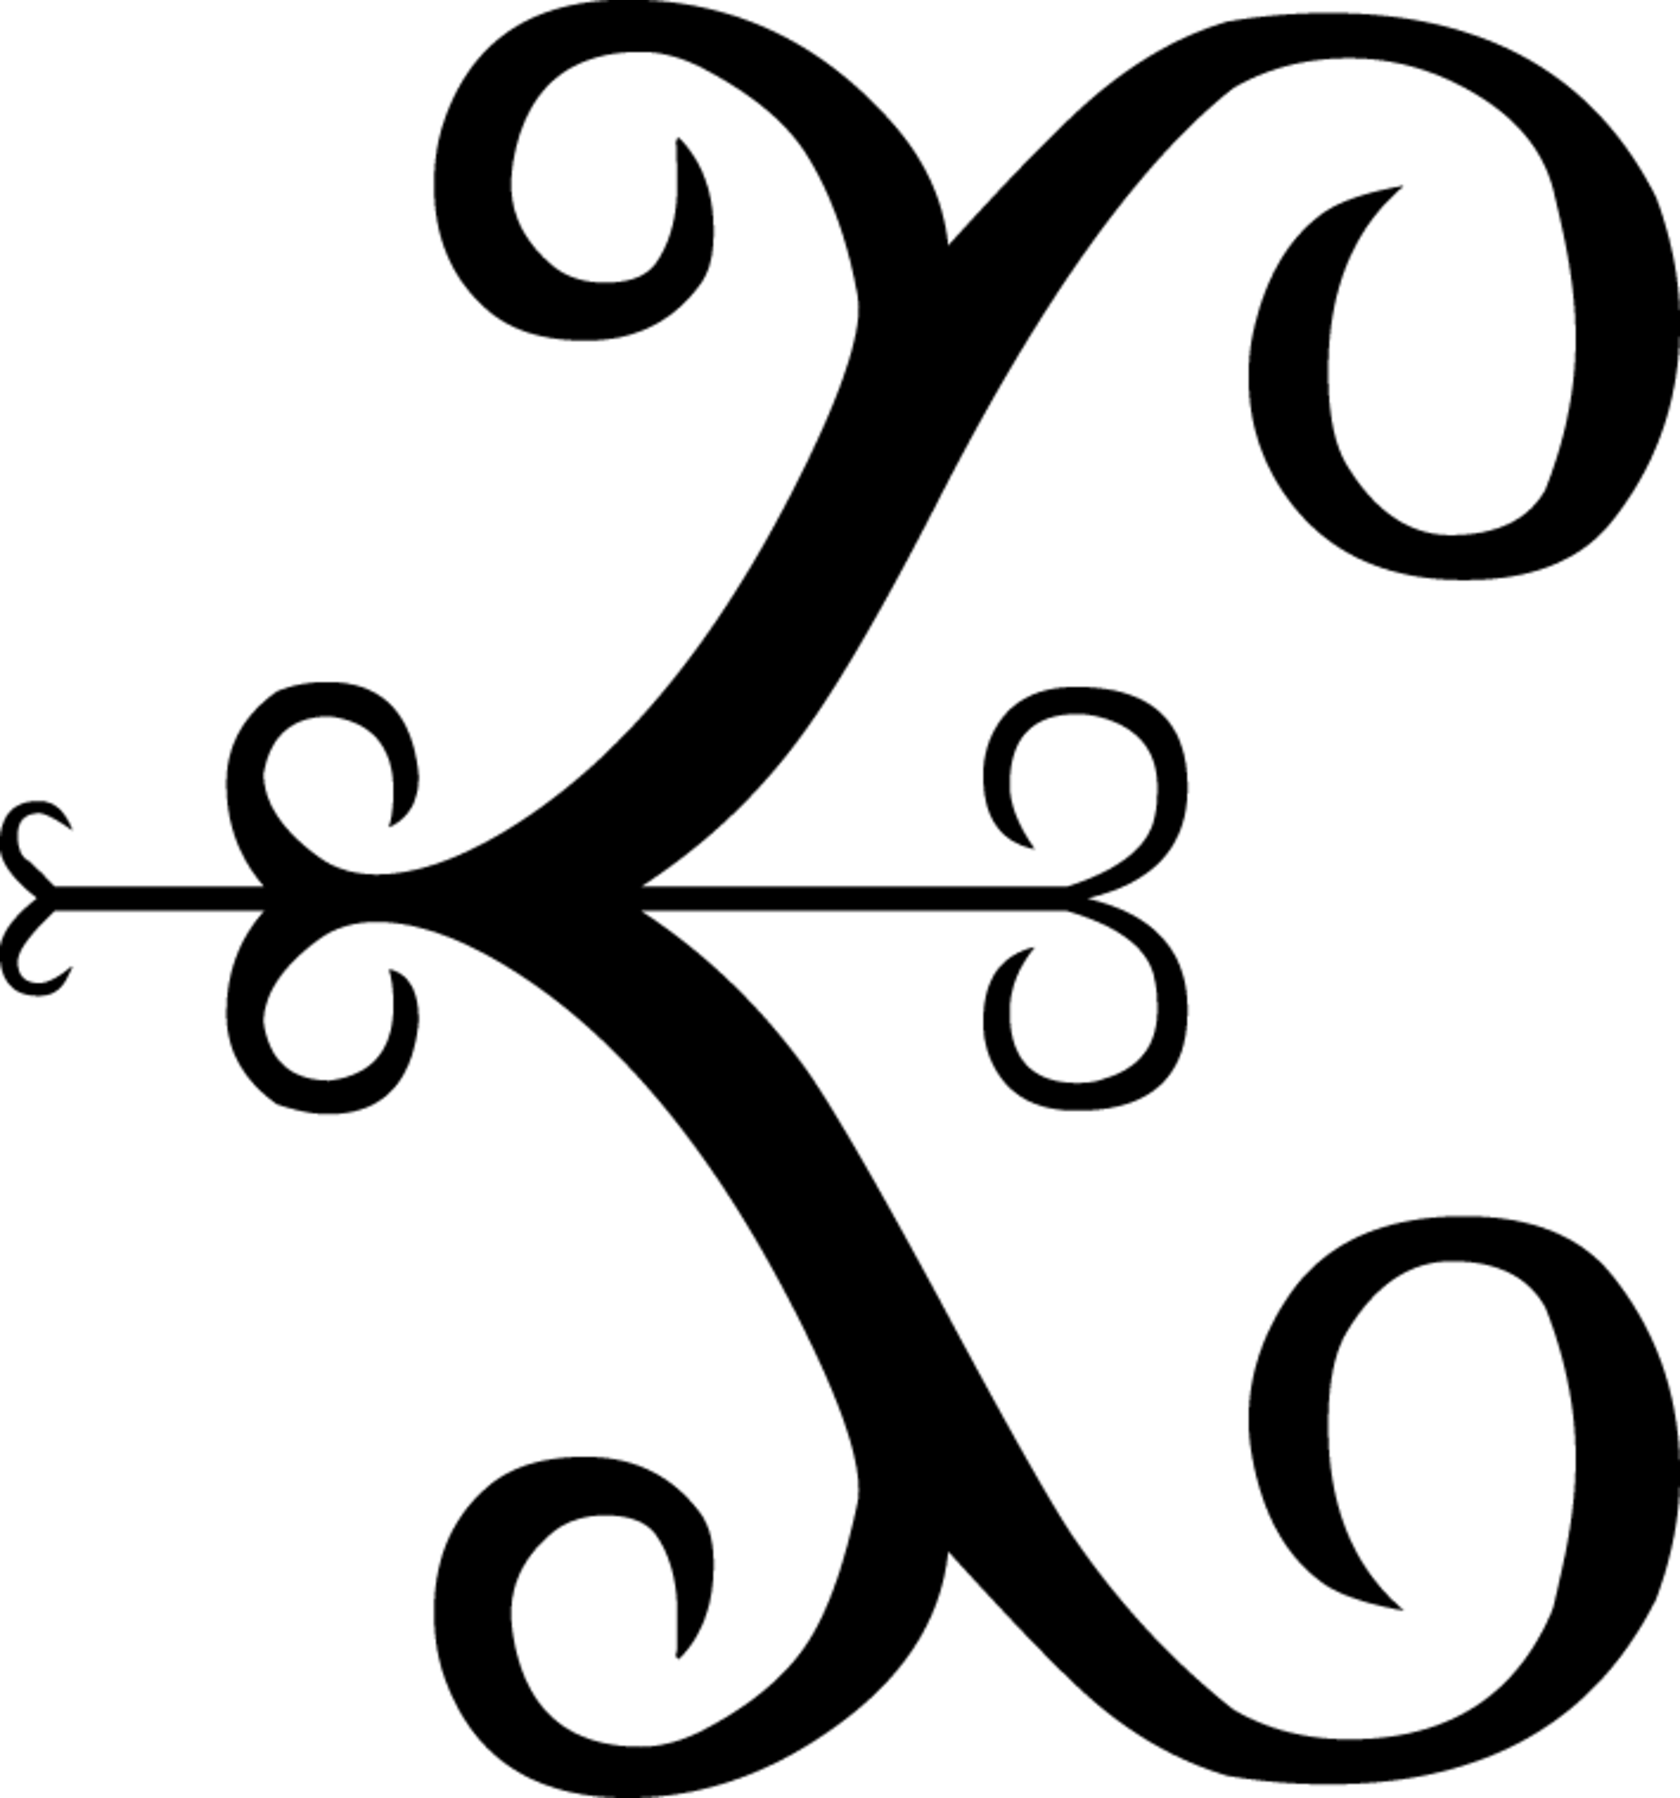
\includegraphics[width=1\textwidth]{./bilder/large_E.png}
    \end{figure}

\end{titlepage}


\newpage

% 
\begin{textblock*}{3cm}(8.8cm,0.6cm) % {width}(x, y)
   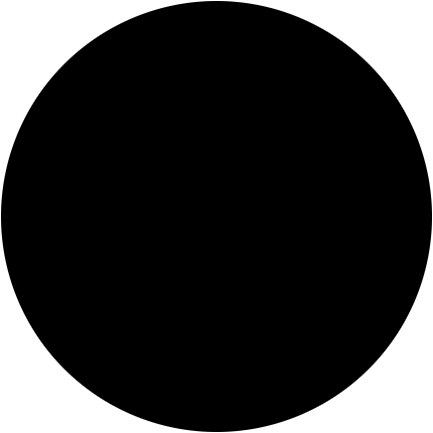
\includegraphics[width=1.0cm]{./bilder/cirkel.png}
\end{textblock*}

\vspace*{-8mm}
Borra ett hål här i pärmen för att fästa din penna: %{\Huge $\bullet$}

\subsubsection*{Konsten att sjunga!}
Att sjunga är verkligen något av det roligaste som finns\dots

Morris Thånell BME19 och Elin Helmersson E21\\
Sångbokskommittén 2024



\newpage

Tack till de som hjälpt oss med boken...

\dots

\newpage

% % Save current headsep
% \newlength{\oldheadsep}
% \setlength{\oldheadsep}{\headsep}

% % Reduce headsep and set pagestyle
% \newpage
% \setlength{\headsep}{0pt}
% % \thispagestyle{noheader}

% \newgeometry{top=10pt, bottom=30pt, left=30pt, right=30pt}
% \setlength{\footskip}{15pt} % Decrease to move the footer up



\vspace*{-13mm} % Pull the content upwards (adjust as needed)
\enlargethispage{15mm} % Allow more vertical space at the bottom



% \enlargethispage{1.5cm}  % Adjust as needed

\begin{center}
    \textbf{Viktig information}
\end{center}


\begin{textblock*}{6cm}(6.0cm,1.5cm) % {block width}(x-coordinate, y-coordinate)
  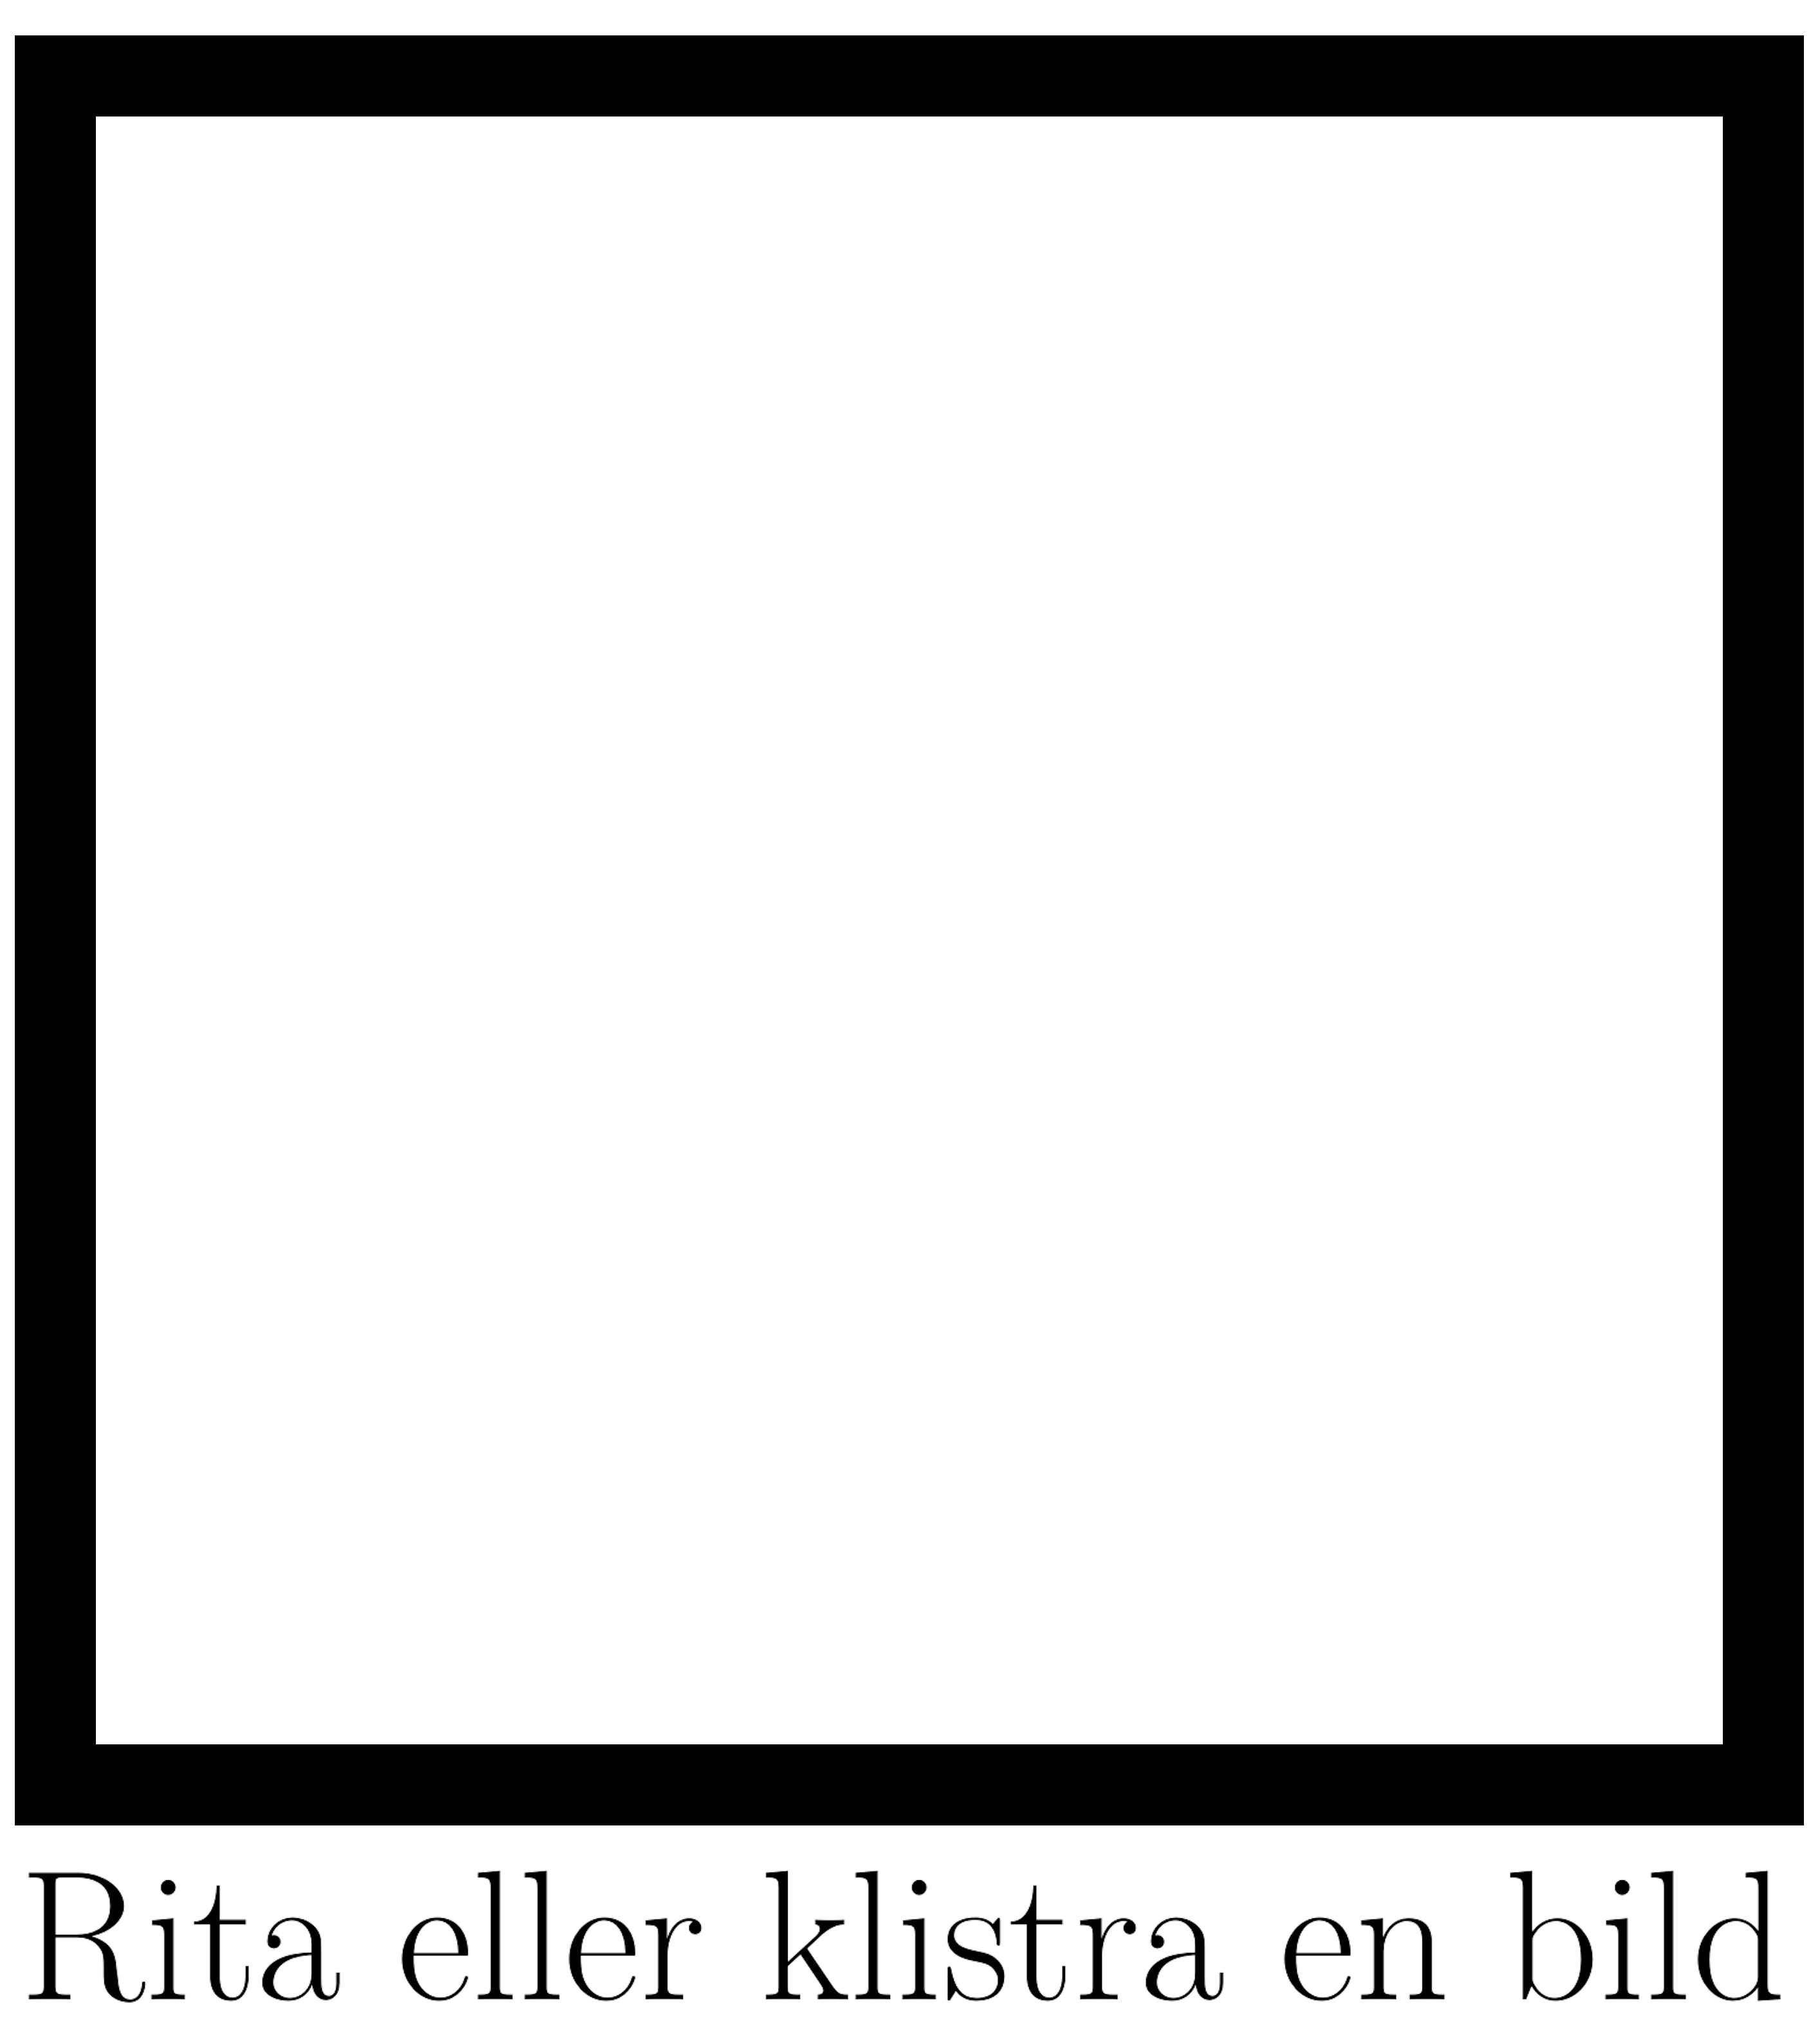
\includegraphics[width=3.5cm]{./bilder/profilbild_stor.png} % Adjust the image size as needed
\end{textblock*}
\vspace*{3.0mm}
\begin{parse lines}[\noindent]{#1\\\vspace{0.5mm}}
  Ägare:\vspace{2mm}
  Program:\vspace{2mm}
  Inskrivningsår:\vspace{2mm}
  Födelsedatum:\vspace{2mm}
  Telefonnummer:\vspace{2mm}


  Lämna tillbaka mig till den här adressen:\vspace{8mm}
  Hittelön:
  Jag vill reinkarneras som:
  I mitt förra liv var jag:
  Detta dricker jag helst:
  Bästa barndomsminnet:
  Julklappen jag aldrig fick:
  Mest impulsiva jag gjort:
  Om jag hade en superkraft:
  Bästa partytrick:
  Favoritintegral:
  Min säng är så här bred:
  Första kändis-crush:
  Gör så här för att charma mig:
  Om jag hade fått välja nollningstema:
\end{parse lines}

\newpage
% \subsubsection*{Innehållsförteckning}
\clearpage
\tableofcontents
\thispagestyle{plainnohead}



\newpage

\begin{center}
  \vspace*{1.5cm}
  {\fontsize{20}{20}\textbf{Vett och etikett}}\\
  \vspace{0.7cm}
  {\fontsize{12}{12}\textit{Om den pryde själv får välja}}
\end{center}
\addtocwithheader{Vett och etikett}  % Add entry to TOC and set header
\noBackground
\newpage
\resetBackground

\subsection*{Klädkod}
För att underlätta förmedlingen av vem som ska ha på sig vad använder vi oss av följande namn.\\

\textbf{Truls}: Manlig teknolog\\
\textbf{Trula}: Kvinnlig teknolog\\
\textbf{Trelsa}: För hen som inte vill identifiera sig med någon av ovanstående.

\subsubsection*{Högtidsdräkt - Militäruniform och folkdräkt}

\textbf{Truls}: Militäruniform, folkdräkt eller frack\\
\textbf{Trula}: Militäruniform, folkdräkt eller balklädding\\
\textbf{Trelsa}: Se Truls/Trula

\subsubsection*{Civil högtidsdräkt}

\textbf{Truls}: Frack, vit skjorta, vit fluga\\
\textbf{Trula}: Balklädding\\
\textbf{Trelsa}: Se Truls/Trula

\subsubsection*{Smoking}
\textbf{Truls}: Smoking, vit skjorta, svart fluga\\
\textbf{Trula}: Lång klänning, dock behöver den inte vara lika elegant som en Balklädding. Tänk festligt.\\
\textbf{Trelsa}: Se Truls/Trula

\subsubsection*{Mörk kostym}
\textbf{Truls}: Mörkblå, mörkgrå eller svart kostym. Vit skjorta med sidenslips eller fluga i valfri färg.\\
\textbf{Trula}: En finare känning, men även byxdress elelr halvlång kjol med jacka går bra.\\
\textbf{Trelsa}: Se Truls/Trula

\subsubsection*{Kavaj}
Ibland även kallad bruten elelr udda kavaj.\\
\textbf{Truls}: Kavaj och ett par finare byxor (dock inte kostymbyxor), skjorta i valfri färg. Fluga eller slips kan vara trevligt!\\
\textbf{Trula}: Cocktailklänning, kjol eller dress.\\
\textbf{Trelsa}: Se Truls/Trula

\subsubsection*{Ouverall}
\textbf{Truls}: Ouvve\\
\textbf{Trula}: Ouvve\\
\textbf{Trelsa}: Se Truls/Trula


\newpage


\subsection*{Vid bordet}
Han har sin bordsdam till höger om sig och hon har sin bordsherre till vänster.
Herren drar ut stolen till höger för att hjälpa sin bordsdam till bords eller från bordet.
\\

Damens väska hängs i första hand över stolsryggen, armstödet eller damens axel.
Alternativt kan väskan placeras mellan ryggen och stolsryggen eller i knäet.
Den serverade maten får inte påbörjas utan värdens tillåtelse.
Vid större sittningar uppmanar en bra värd de sittande att äta direkt av rätter som skall förtäras varma.
Innan maten har påbörjats får man dricka av vattenglaset samt bryta och äta eventuellt bröd som serverats.
\\

Ditt vattenglas är alltid placerat längst till höger, sedan används glasen från höger till vänster i takt med att rätterna påbörjas.
Värden bestämmer när en rätt påbörjas.
Servetten du får till bords skall placeras i knäet innan först rätten påbörjas. Den skall placeras på stolen då du lämnar bordet innan sittningens slut, absolut inte på bordet.
Vid sittningens sult läggs servetten upp på vänsersidan av tallriken, lätt skrynklad.
\\

\newpage

Besticken används i ordningen "utifrån och in".
Besticken till förrätten ligger således ytterst.
Vid rätter som kräver sked så ligger skeden på höger sida om tallriken, förrutom vid dessert.
Alla dessertbestick finns ovanför tallriken.
Om det ligger en gaffel till höger sida om tallriken så betyder det att rätten enbart äts med gaffel.
Besticken får inte placeras lutande mellan bordet och tallriken, utan esticken förblir på tallriken när de har börjat användas. 
Då besticken ät placerade på tallriken som klockslaget tjugo i fyra betyder det att du fortfarande äter,
medan klockslaget tjugo över fyra betyder att du är klar.
\\

Vid bal och finare sittningar är det brukligt att ha med sig en present till sin bordsgranne. 
En fun fact är att begreppet "vänterprassla" kommer just från att det fanns/finns vissa herrar som inte kunde/kan hålla sig till sin bordsdam, 
utan istället såg/ser sig om till vänster for att prova lyckan där.


\vissteduatt{Visste du att bordsherre och bordsdam är bordsplaceringsbenämningar\\ som avser att underlätta sittningsförfarande och är helt könsneutrala?}

\newpage

\subsection*{Skålen}

När det skålas och det ska skålas korrekt så börjar man 
med att skåla med sin bordsgranne, sedan med din sekundära 
bordsgranne och slutligen rakt över till den mittemot. 
Efter dricker man ur och upprepar denna process, fast baklänges.
\\

Alltså:
Han börjar till höger,

sedan vänster och slutligen rakt fram.

Hon börjar till vänster,

sedan höger och slutligen rakt fram.

Drick, sedan alltsammans baklänges.

\vissteduatt{En myt säger att man får börja äta av maten vid fler gäster än\\
åtta vid bordet, detta är fel!}

\newpage

\subsection*{Underhållning}
På sittningar bjuds det utöver mat och dryck (som man förvisso betalt för) oftast även på underhållning.
Denna kan yttra sig antingen som sång från Sångförmännen eller i form av ett spex.
Till dessa akter finns det ett par förhållningsregler att beakta.
\\

1. När Sångförmännen talar, är man tyst.\\
2. När Sångförmännen sjunger, sjunger man med.\\
3. När Sångförmännen drar ett skämt, skrattar man.\\
4. När det är spex, är man tyst.\\
5. Punkt 4 får brytas om spexet är så roligt att man behöver skratta. Då skrattar man.\\
6. Har man varit på toaletter väntar man till spexet är fördigt innan man sätter sig till bords igen.\\
7. Behöver man gå på toaletten under ett spex - bad luck.\\
8. Vill man spexa på en sittning anmäler man det i god tid till Sångförmännen.\\
9. Spontansång beivras!\\
10. Spontansång uppmuntras om Sångförmännen meddelat satt sången är fri. Då gäller inte Punkt 9.\\
11. Tempo är okej om Sångförmännen sagt att det är det.\\
12. Tempo är inte okej om Sångförmännen sagt att det inte är det.\\
13. Har sångförmännen inte sagt något om Tempo lär de göra det snart.\\
\\


\newpage

Efter ett spex visar de sittande sin uppskattning genom att be spexarna att spexa en gång till.
Detta görs genom att sjunga nedanstående sång, som initieras av Sångförmännen.
\\

\begin{parse lines}[\noindent]{\textit{#1}\\}
  Det där det gjorde han/hon/de fan så bra, hej!
  En skål uti botten för honom/henne/dem nu vi ta
  Och alla så dricka vi nu [namn på spexare/spexarna eller mumlande] till 
\end{parse lines}

Den sista raden upprepas till det att spexaren eller spexarna svarar:
\\

\begin{parse lines}[\noindent]{\textit{#1}\\}
  Och namn på spexare/spexarna spexar gärna en gång till.
\end{parse lines}

Efter det andra spexet är det dock färdigspexat, men självfallet ska de sittande 
ändå ännu en gång visa sin uppskattning genom en sång, som även den initieras av Sångförmännen.
\\

\subsection*{Ettans gutår}
\begin{parse lines}[\noindent]{#1\\}
  Det var i vår ungdoms fagraste vår
  Vi drack varandra till och vi sade Gutår
\end{parse lines}


\newpage

\subsection*{Mer om teknologens utstyrsel}
Det kan trots föregående sidors fenomenala utlägg ibland kanske vara lite förvirrande att avgöra vad man ska ha på sig.
Men något som alltid går hem i Teknlogsammanhang är självfallet Teknologmössan.
Denna kan och bör man bära oavsett tillställning.
\\

Teknologmössan får dock enbart pryda de teknologer som med någorlunda bravur genomfört Nollningen på TLTH.
Och likt fjällräven med sin vinterpäls och sommarpäls är det av största vikt att även Teknologen skiftar mellan sin vita sommarmössa och sin mörkblåa vintermössa.
Men till skillnad från fjällräven så finns det för teknologen väldefinierade datum för när den ena eller den andra mössan ska användas.
\\

\textbf{Sommarmössa: 1:a maj - 3:e oktober}

\textbf{Vintermössa: 4:e oktober - 30:e april}
\\

Viktigt att notera är dock att oavsett årstid så används den vita sommarmössan då Högtidsdräkt bärs.
\\

För att lättare hålla koll på vilka datum som gäller bör man inte jämföra med vilka datum som det är tillåtet att ha dubbdäck på sin bil, för det är bara nästan samma datum.

\newpage

\subsection*{Plösen}
Som den observante noterar så är teknologmössan berikad med en lös där ett tofsprytt snöre hänger försynt och dinglar.
På detta snöre fäster man efter varje påbörjat läsår en spegat. En vit spegat för de som studerar Elektroteknik och en rödvit spegat för de som studerar Medicin och Teknik.
Det finns även en svart som indikerar sabattsår, en skogsgrön för ett år i lumpen och en vit-blå-silver som visar att man spenderat ett år som heltidare i Teknologkårens tjänst.
\\

Utöver att hålla rätt antal spegater på rätt plats är det av yttersta vikt att själva tofsen hålls fräsch. Ett bra sätt att göra detta är att låta andra individer knyta knutar av trådarna på tofsen. Detta slitgöra borde så klart belönas med en fin puss.
Är man i förhållande och inte känner för att pussa en massa folk kan man göra en knut av själva snöret ovanför spegaterna för att signalera detta.
\\

\subsection*{Elektroslajd}
Ta på dig ouvven.\\
Släng dig ner för backen.\\
Gör ouvven fin.

\newpage


% \subsubsection*{Hur man är på sittning}
% \subsubsection*{REGLER}

% \subsubsection*{Mellanskål}

% Nu är det dags för mellanskål
% Om det så är det sista jag gör
% Nu är det dags för mellanskål
% Hoppas inte föräldrarna stör
% Nu är det slut på versen 
% Det är dags för mellanskål

% \newpage

% \subsection*{Hur man tågar}

% När ett stort antal teknologer behöver förflytta sig till fots, kan detta göras genom att tåga. 
% När man möter ett övergångsställe stannar delar av tåget med jämna mellanrum för att låta bilar passera.
% När man tågar håller man sig åt sidan av vägen där man går så att cyklar och andra kan åka förbi.

% När man tågar ska man såklart sjunga, och här passar E-sektionens kampvisor mycket väl.

% En annan låt som gärna sjunges är den här under. 

% Oh ale ale
% a riki tiki tamba
% a massa massa massa
% baloe baloe baloe
% I said baloe baloe baloe




% \newpage

\subsection*{Ordförande}
Ordförande har till uppgift att leda och representera sektionen och en massa andra saker. 
Detta är dock inte alls lika viktigt om man ställer det mot förväntningarna som finns på Ordförande när han/hon/hen sjunger Taggig Blomma! 
Man får aldrig låna ut sin sångbok till Ordförande när denne skall sjunga Taggig Blomma ty då får man aldrig se den igen.
\\

\vspace{1cm}

\subsection*{Taggig Blomma} 
\index[alfa]{Taggig Blomma}
\index[anfa]{När man söker LTH att glömma...}
\songinfo{Mel: Rosen \\Text: Jan Grenner F71}

\begin{parse lines}[\noindent]{#1\\}
  När man söker LTH att glömma,
  är det skönt att glaset sitt få tömma
  Glömma att alla studier gått på sne’
  och att tentamen gick åt helvete

  För just nu idag, så köpte jag
  en liter sprit och min börs den var tom
  Renat så klart, det var underbart
  att få tömma den i min gom
  
\end{parse lines}

\newpage

\begin{parse lines}[\noindent]{#1\\}
  När jag som vanligt gick till bolaget
  för att bota mina abstinensbesvär
  så svarade dom helt enkelt: "Nej,
  det skall nog inte vara mera här
  Ni är ju full och för ung
  Har ni legitimation?
  Utan den får ni minsann ingen flytande muntration"
  
  Men ingenting kunde hindra mig
  jag måste ha gök ikväll
  På stan jag drev tills en langare jag såg
  i bil av senaste modell
  Flaskan blänkte, kapsylen blixtrade i dess topp
  Darrhänt jag tänkte:
  "De' va' faan va' korken va' svår att få opp!"
  
  När man söker...
  
\end{parse lines}

\newpage

\enlargethispage{1.0cm}
\subsection*{Några ord om akademisk kvart}

{\fontsize{9}{9}\selectfont 
Förr i världen på den tid då bilar och varmvattenberedare var exotiska, 
så var man ganska dålig på att hålla rätt på tider. 
Anledningen till detta var att det fanns en stor brist på klockor, fickur och mobiltelefoner. 
I både Lund och Uppsala, emellertid, var man bortskämda med stora domkyrkor. 
Varje heltimme ringde (och gör fortfarande) kyrkklockorna åtta gånger, 
och då visste man som student att det var dags för föreläsning. 
Men självfallet tog det ju en liten stund att ta sig till föreläsningssalen, 
och det visade sig att oavsett var man ursprungligen befann sig tog det alltid exakt en kvart att förflytta sig. 
Okej, kanske inte exakt, men det lilla dröjsmålet som det innebar att själv inte ha koll på tiden resulterade i införandet av den akademiska kvarten.
Och traditionsbundna och morgontrötta som vi studenter är, 
så är detta ett fenomen som än idag lever kvar. Så om det står att en föreläsning börjar kl 8, 
betyder det att den egentligen börjar kl 8:15. 
Om man nu verkligen vill att studenterna ska infinna sig på ett ställe vid exakt kl 8 
(tentor, många laborationer, m.m.), så anger man det genom att antingen skriva ut hela klockslaget, 
som i "kl 8:00", eller genom att skriva "prick" efteråt, som i "kl 8 prick", alternativt "kl 8 (..)". 
Och för att krångla till det ytterligare så finns även något som kallas akademisk dubbelkvart. 
Detta infaller på vardagar efter kl 18:00 och på helger. 
Det är i princip samma regler som för den enkla akademiska kvarten, 
men det är en halvtimmes fördröjning istället. 
En sittning som börjar kl 19 börjar alltså i själva verket kl 19:30. 
Och vill man att gästerna ska komma exakt kl 19, 
så skriver man åter en gång antingen ut hela klockslaget, 
som i "kl 19:00", eller lägger till "prick" efteråt, som i "kl 19 prick", alternativt "kl 19 (..)".
}

\newpage


\subsection*{Social for Dummies}
När man är på en sittning är det viktigt att man är social med sina bordsgrannar. 
Ofta är det så att man inte känner någon bordsgranne sen tidigare och vid sådana 
fall kan det vara lite svårt att vara social. Därför har Social for Dummies 
skapats för att lätta på spänningen.
\\

För att kunna vara social så måste man kunna kommunicera med dem i sin omgivning. 
Detta görs enklast oralt. Förutom att introducera sig och fråga bordsgrannarna vad de 
heter och pluggar kommer nu några bra samtalsämnen samt frågor.
\\
\begin{itemize}[itemsep=0.0em]
  \item Dagens konjunkturläge
  \item Microsoft vs. Apple vs. Linux?
  \item Vädret. Finns det inget väder, prata om tryck.
  \item Politiska läget på Island?
  \item Kan björnar klättra?
  \item Det stoltaste du gjort i trä– eller syslöjden?
  \item Vad hade du jobbat som om du var utomjording?
  \item Vad är det galnaste du gjort?
\end{itemize}


Skulle det vara så att din bordsgranne är något av en s.k. Gamer, så finns följande sida för sådana.

Reglerna för \textit{Luffarschack} kan förhoppningsvis Gamern.

OBS! Använd gärna blyerts!

\newpage

\thispagestyle{plainnohead}

\phantom{osynlig text}

\begin{textblock*}{3cm}(1.0cm,1.0cm) % {width}(x, y)
   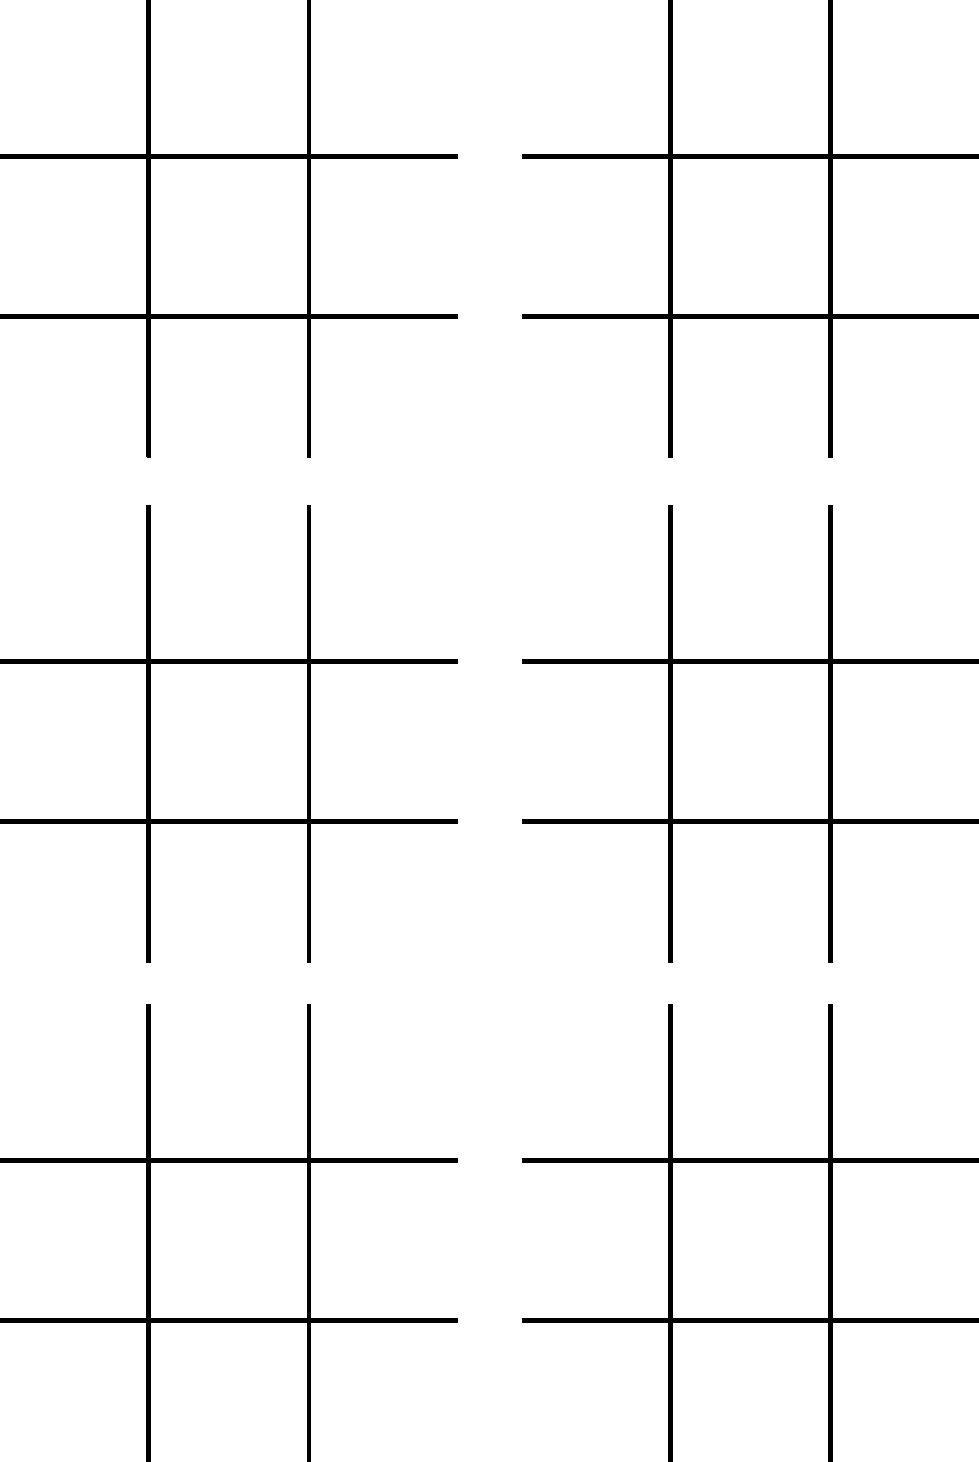
\includegraphics[width=8.5cm]{./bilder/luffarschack.png}
\end{textblock*}


\noBackground

\newpage
\resetBackground

\thispagestyle{plainnohead}

\vspace*{-13mm} % Pull the content upwards
\enlargethispage{15mm} % Allow more vertical space at the bottom

\begin{center}
    \normalfont\normalsize\bfseries Bordsgranne of Fame
\end{center}

Namn: \hspace{2.5cm} Sittning: 

% \newpage
% \setlength{\topskip}{0pt}  % Remove the top skip
\vspace*{0.3cm}
\rule{\textwidth}{0.0mm}
\vspace*{0.65cm}
\rule{\textwidth}{0.4mm}
\vspace*{0.65cm}
\rule{\textwidth}{0.4mm}
\vspace*{0.65cm}
\rule{\textwidth}{0.4mm}
\vspace*{0.65cm}
\rule{\textwidth}{0.4mm}
\vspace*{0.65cm}
\rule{\textwidth}{0.4mm}
\vspace*{0.65cm}
\rule{\textwidth}{0.4mm}
\vspace*{0.65cm}
\rule{\textwidth}{0.4mm}
\vspace*{0.65cm}
\rule{\textwidth}{0.4mm}
\vspace*{0.65cm}
\rule{\textwidth}{0.4mm}
\vspace*{0.65cm}
\rule{\textwidth}{0.4mm}
\vspace*{0.65cm}
\rule{\textwidth}{0.4mm}

\noBackground

\newpage
\resetBackground




\subsubsection*{Tankar på vad vi vill lägga till}

\subsubsection*{Mellanskål}
Ibland när man sjunger en väldigt lång låt (se The Engineer's Drinking Song) kan det vara så att man behöver vattna strupen under låtens gång. Såklart vill man inte behöva missa en vers bara för att man behöver dricka. Då kan man mellan två verser sjunga låten nedan för att få utbringa en skål, innan man fortsätter sjunga igen.

\subsection*{Mellanskål} 
\index[alfa]{Mellanskål}
\index[anfa]{Mellanskål}
\songinfo{Mel: Fredagsmys}

\begin{parse lines}[\noindent]{#1\\}
    Det dags för mellanskål
    Om det så är det sista jag gör
    Snart är det mellanskål
    Hoppas inte föräldrarna stör
    Nu är det slut på versen 
    Det är dags för mellanskål
\end{parse lines}


\subsection*{Hur man tågar}

När ett stort antal teknologer behöver förflytta sig till fots, kan detta göras genom att tåga. 
När man möter ett övergångsställe stannar delar av tåget med jämna mellanrum för att låta bilar passera.
När man tågar håller man sig åt sidan av vägen där man går så att cyklar och andra kan åka förbi.

När man tågar ska man såklart sjunga, och här passar E-sektionens kampvisor mycket väl.

En annan låt som gärna sjunges är den här under. 

Oh ale ale
a riki tiki tamba
a massa massa massa
baloe baloe baloe
I said baloe baloe baloe


\subsubsection*{Dubbelkolla att det är andra upplagan}
Hör av oss till förra Sångbokskommittén och fråga om detta är andra upplagan. Vad fanns innan detta?


\newpage
\subsection*{Rita dig själv}

% \begin{textblock*}{6cm}(4cm,5.0cm) % {block width}(x-coordinate, y-coordinate)
%   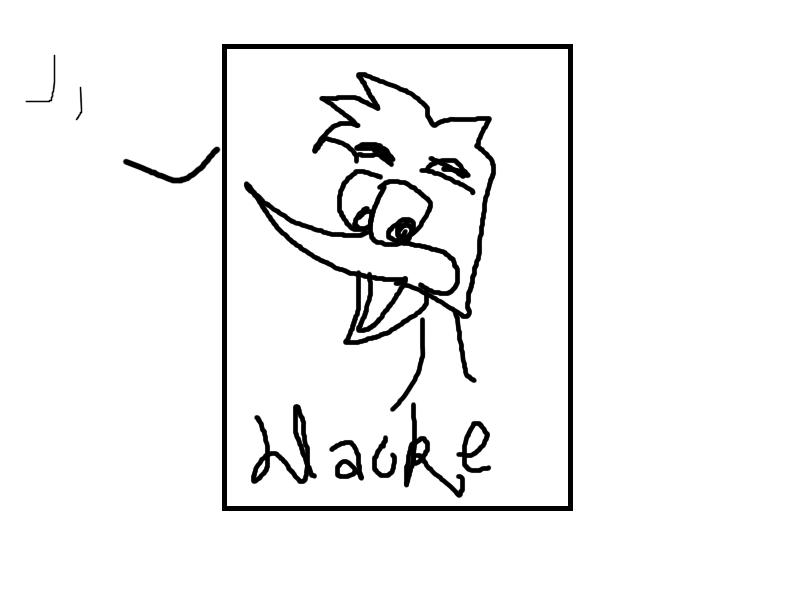
\includegraphics[width=5.5cm]{./bilder/Untitled.png} % Adjust the image size as needed
% \end{textblock*}

Gör som Hacke och rita dig själv i någon annans bok!

\begin{textblock*}{6cm}(1.55cm,3.45cm) % {block width}(x-coordinate, y-coordinate)
  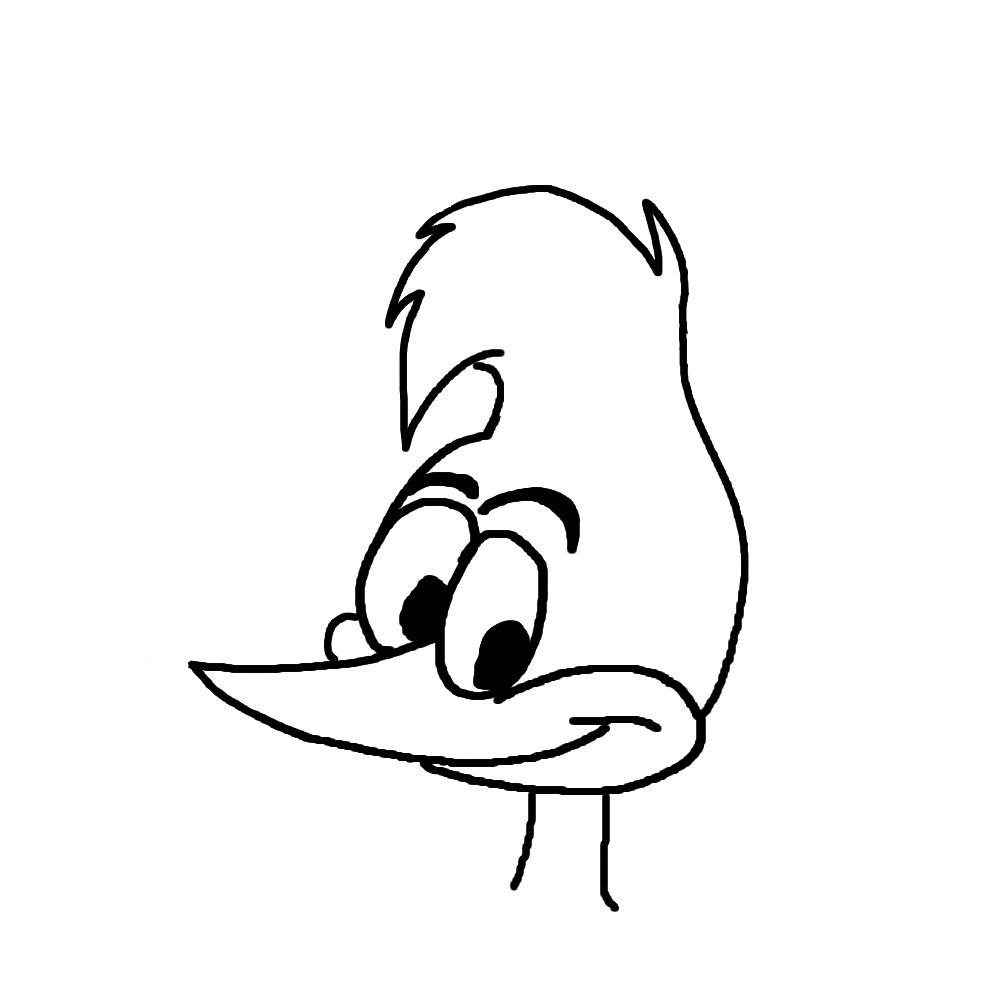
\includegraphics[width=2 cm]{./bilder/ramar/hacke_portratt_2.png} % Adjust the image size as needed
\end{textblock*}



\begin{textblock*}{6cm}(1cm,2.7cm) % {block width}(x-coordinate, y-coordinate)
  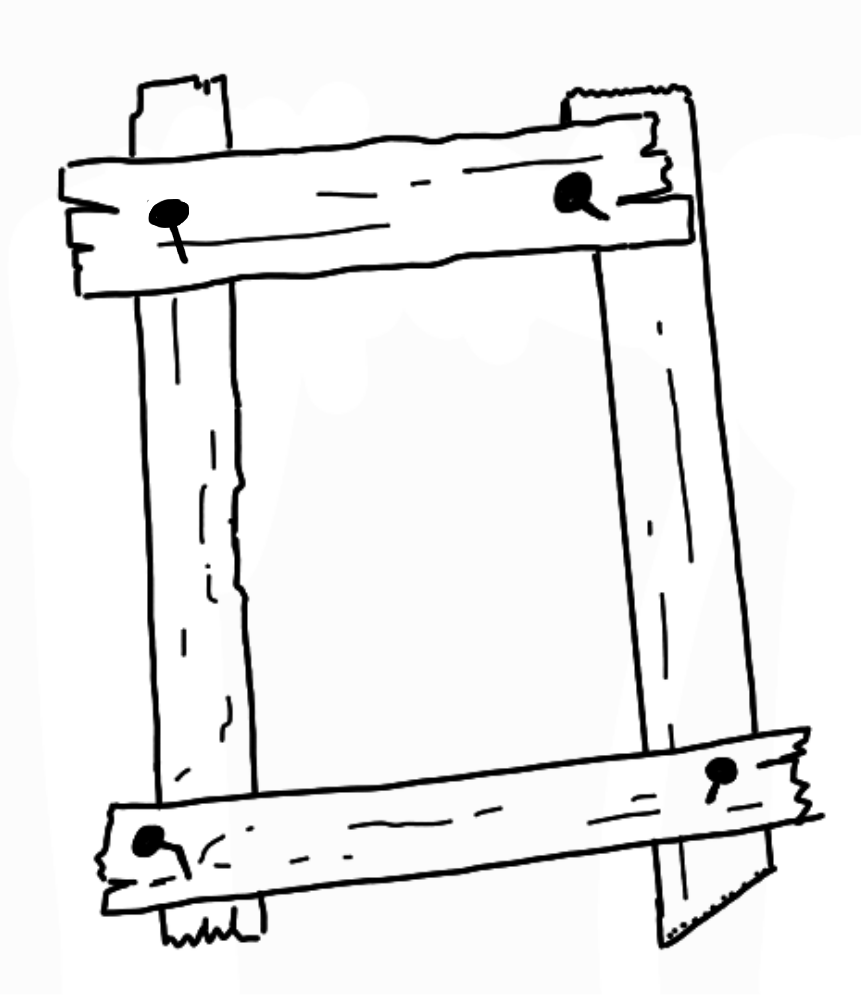
\includegraphics[width=3cm]{./bilder/ramar/Ram4.png} % Adjust the image size as needed
\end{textblock*}

\begin{textblock*}{6cm}(4cm,2.7cm) % {block width}(x-coordinate, y-coordinate)
  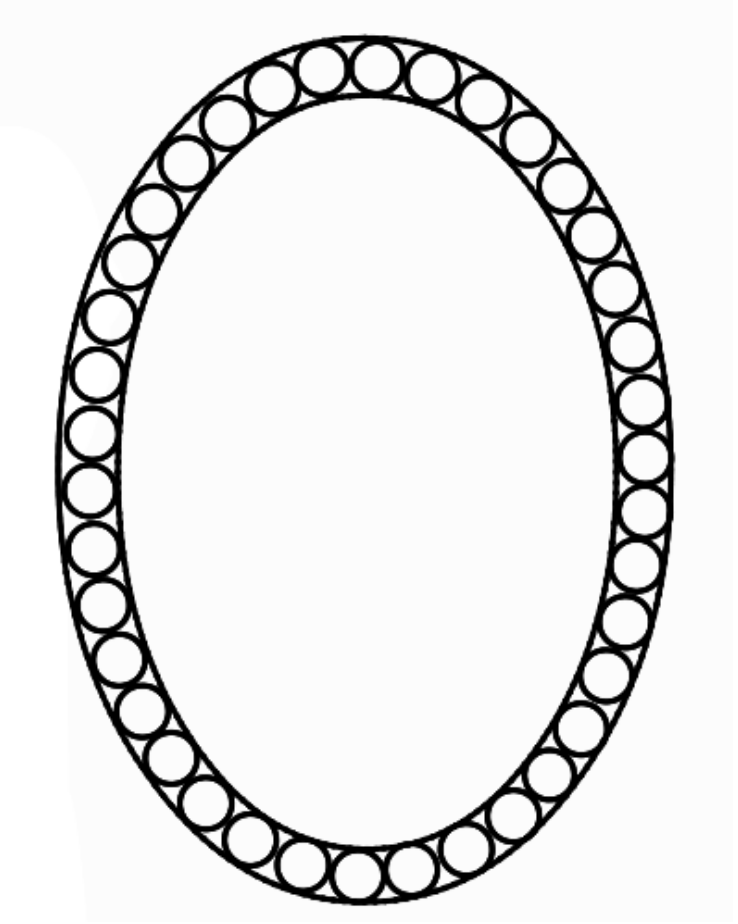
\includegraphics[width=2.6cm]{./bilder/ramar/Ram5.png} % Adjust the image size as needed
\end{textblock*}

\begin{textblock*}{6cm}(6.6cm,3.2cm) % {block width}(x-coordinate, y-coordinate)
  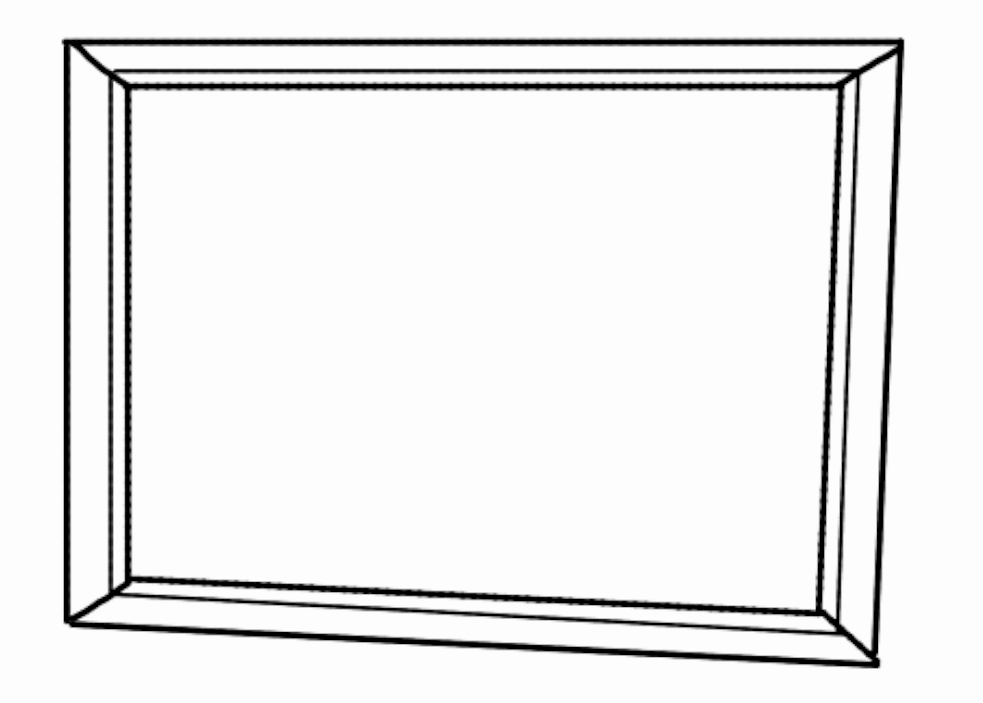
\includegraphics[width=3.5cm]{./bilder/ramar/Ram6.png} % Adjust the image size as needed
\end{textblock*}



\begin{textblock*}{6cm}(0.8cm,6.4cm) % {block width}(x-coordinate, y-coordinate)
  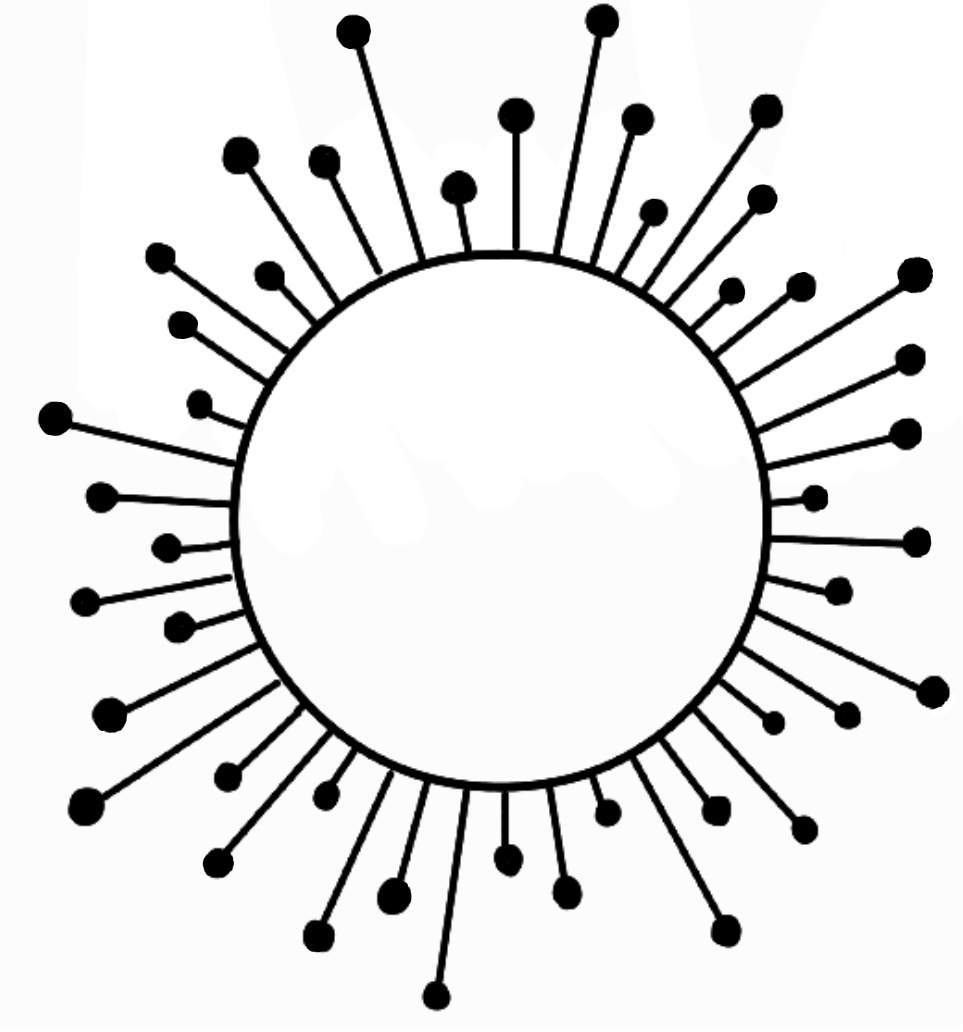
\includegraphics[width=3.3cm]{./bilder/ramar/Ram7.png} % Adjust the image size as needed
\end{textblock*}

\begin{textblock*}{6cm}(4.2cm,6.2cm) % {block width}(x-coordinate, y-coordinate)
  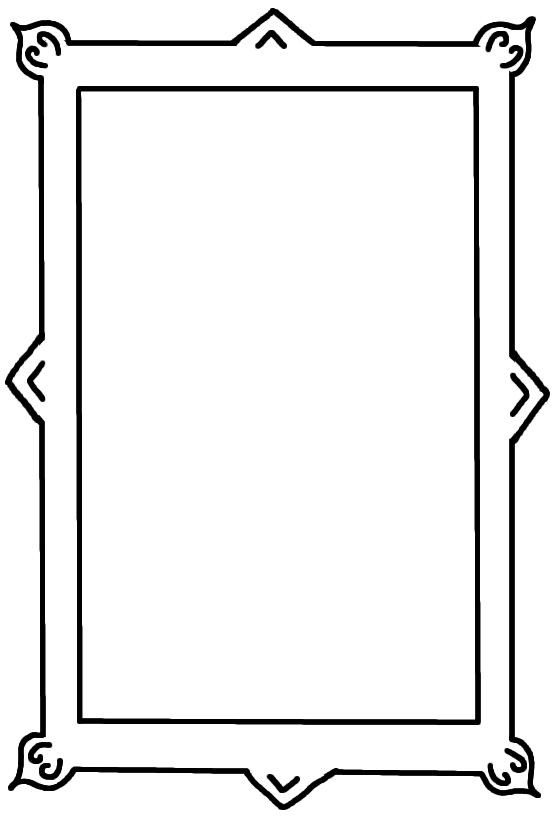
\includegraphics[width=2.5cm]{./bilder/ramar/ram1.png} % Adjust the image size as needed
\end{textblock*}

\begin{textblock*}{6cm}(6.9cm,6cm) % {block width}(x-coordinate, y-coordinate)
  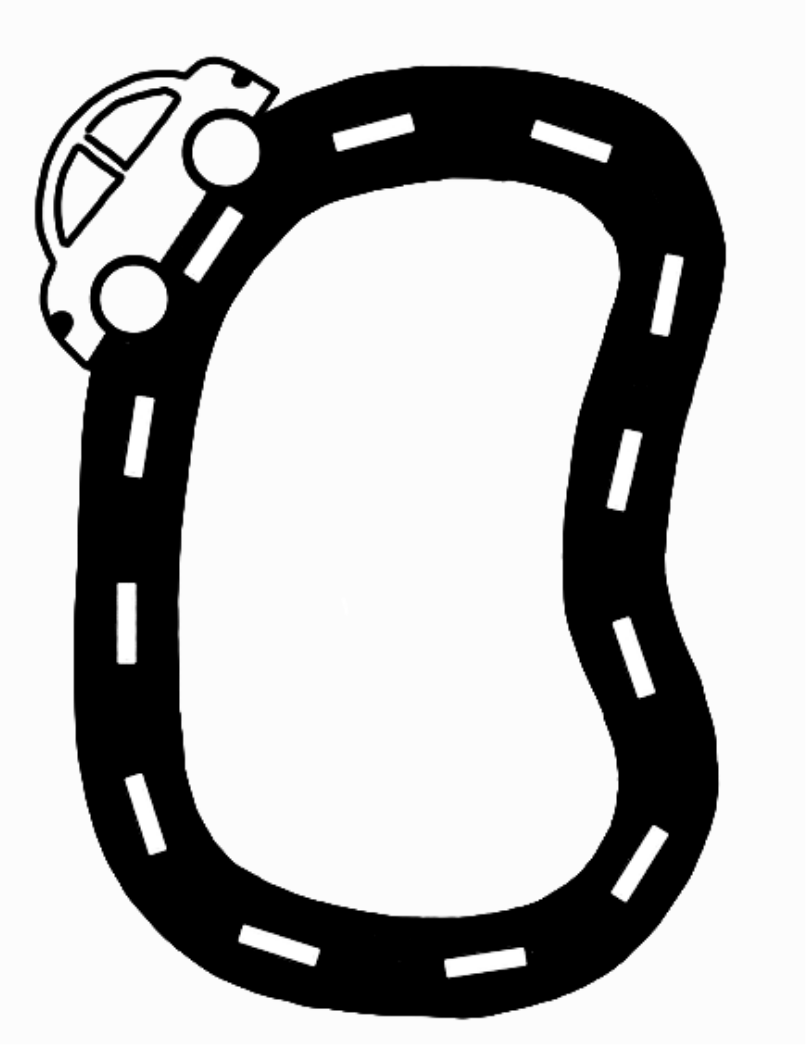
\includegraphics[width=2.8cm]{./bilder/ramar/Ram8.png} % Adjust the image size as needed
\end{textblock*}



\begin{textblock*}{6cm}(1.1cm,10.3cm) % {block width}(x-coordinate, y-coordinate)
  \includegraphics[angle=-90, width=3.2cm]{./bilder/ramar/Ram3.png} % Adjust the image size as needed
\end{textblock*}

\begin{textblock*}{6cm}(4.4cm,10.1cm) % {block width}(x-coordinate, y-coordinate)
  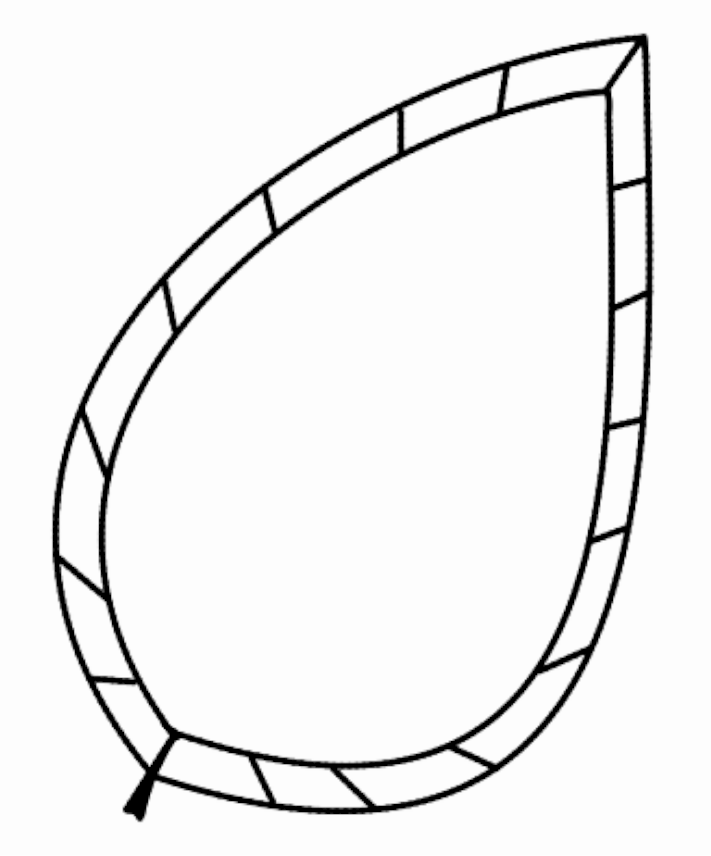
\includegraphics[width=2.6cm]{./bilder/ramar/Ram9.png} % Adjust the image size as needed
\end{textblock*}

\begin{textblock*}{6cm}(7.1cm,9.8cm) % {block width}(x-coordinate, y-coordinate)
  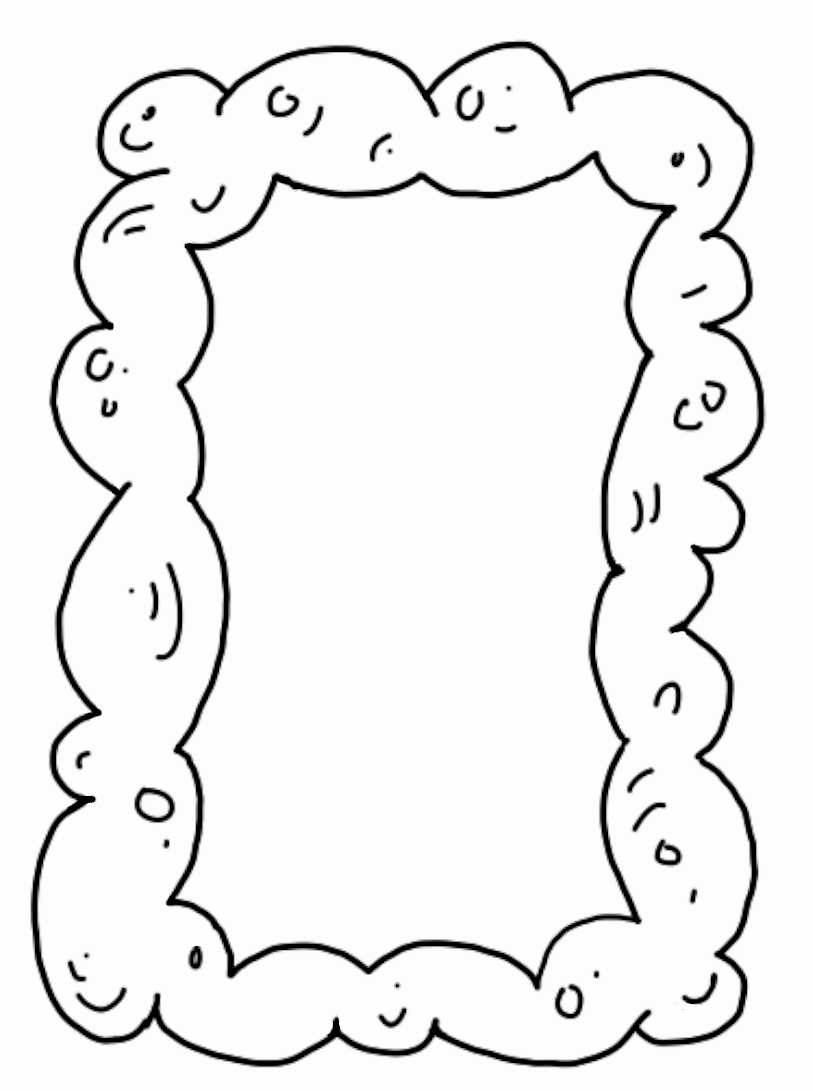
\includegraphics[width=2.8cm]{./bilder/ramar/Ram10.png} % Adjust the image size as needed
\end{textblock*}

\newpage

% tom sida

% \newpage

% \input{kapitel/XX-sånger.tex}
%\input{kapitel/XX-nya_låtar.tex}

\begin{center}
    \vspace*{1.5cm}
    {\fontsize{20}{20}\textbf{E-sektionens visor}}\\
    \vspace{0.7cm}
    {\fontsize{12}{12}\textit{Om E:aren själv får välja}}  
\end{center}
\addtocwithheader{E-sektionens visor}  % Add entry to TOC and set header
\noBackground

\newpage
\resetBackground


\subsection*{E-sektionens Kampvisa I}
\index[alfa]{E-sektionens Kampvisa I}
\index[anfa]{Det sprakar så glatt i vårt hår}
\songinfo{Mel: Stars and Stripe \textbf{OSÄKER MELODI?}}

\begin{parse lines}[\noindent]{#1\\}
    Det sprakar så glatt i vårt hår
    ur öronen sprutar det gnistor
    och strömmarna i våra tår
    laddar upp oss när vi går.

    I hjärnan vi har resistans
    och ström genom motstånd ger en spänning
    och spänning det vill vi ju ha.
    Vi går på E! Vi går på E!
    Vi går på Elström!

\end{parse lines}


\subsection*{E-sektionens Kampvisa II} 
\index[alfa]{E-sektionens Kampvisa II}
\index[anfa]{E, E, E vill vi se}
\songinfo{Mel: Trink, trink, brüderlein trink}

\begin{parse lines}[\noindent]{#1\\}
    E, E, E vill vi se
    E är det bästa där é
    E, E, E vill vi se
    E får oss alla att le!
    Spänning där é i vär erotik
    vi kör med medicin och teknik.
    Spänning där é i vår erotik
    vi kör med elektroteknik

\end{parse lines}

\vissteduatt{Visste du att E-sektionen har sjukt många kampvisor? ELLER \\Visste dua tt Kampvisa II reviderades för att innefatta båda utbildningarna på E-sektionen?}

% \newpage

\subsection*{E-sektionens Kampvisa III} 
\index[alfa]{E-sektionens Kampvisa III}
\index[anfa]{Vi é elteknister ifrån LTH}
\songinfo{Mel: Vi äro musikanter}

\begin{parse lines}[\noindent]{#1\\}
    Vi é elteknister ifrån LTH.
    Hos oss finns inga brister och dé é ju som så.

    (Att) Vi kan lödda, räkna, dricka, bränna sprit.
    Upp till Lophtet, kom så går vi dit!

    Vi kan räkna tangens, sinus, derivera, integraler.
    Vi kan koda singelchip och mata våran pic.

    Ett in, noll ut, rulla kabel, heja vit!
    Vi vill att just du skall komma hit.

    Hoppa i din vita overall och börja gå.
    Elteknik på LTH det bästa du kan få!

\end{parse lines}


\subsection*{E-sektionens Kampvisa IV} 
\index[alfa]{E-sektionens Kampvisa IV}
\index[anfa]{Vi vill ha mera E}
\songinfo{Mel: Mera mål}

\begin{parse lines}[\noindent]{#1\\}
    Vi vill ha mera E, flera E
    Å E det kommer ni att se
    Vi vill ha mera E, mycket mer
    Se upp här kommer vi från E

\end{parse lines}

\vissteduatt{Visste du att E-sektionen är den äldsta sektionen på LTH?}

\newpage


\subsection*{E-sektionens Kampvisa V} 
\index[alfa]{E-sektionens Kampvisa V}
\index[anfa]{Alla vi på E-sek klappar nu} % VILL VI HA DENNA ENS?
\songinfo{Mel: Klappa händerna}

\begin{parse lines}[\noindent]{#1\\}
    //: Alla vi som går på E-sek klappar nu ://

\end{parse lines}


\subsection*{E-sektionens Kampvisa VI} 
\index[alfa]{E-sektionens Kampvisa VI}
\index[anfa]{Vi går på E-sek}
\songinfo{Mel: Man ska ha husvagn}

\begin{parse lines}[\noindent]{#1\\}
    Vi går på E-sek, och vi har spänning så som få
    Vi går på E-sek, äldst och bäst på LTH
    Vi går på E-sek, vår färg är vit, Elektrovit!
    Vi går på E-sek, LTH:s elit!

\end{parse lines}


\begin{textblock*}{3cm}(3.5cm,8.9cm) % {width}(x, y)
    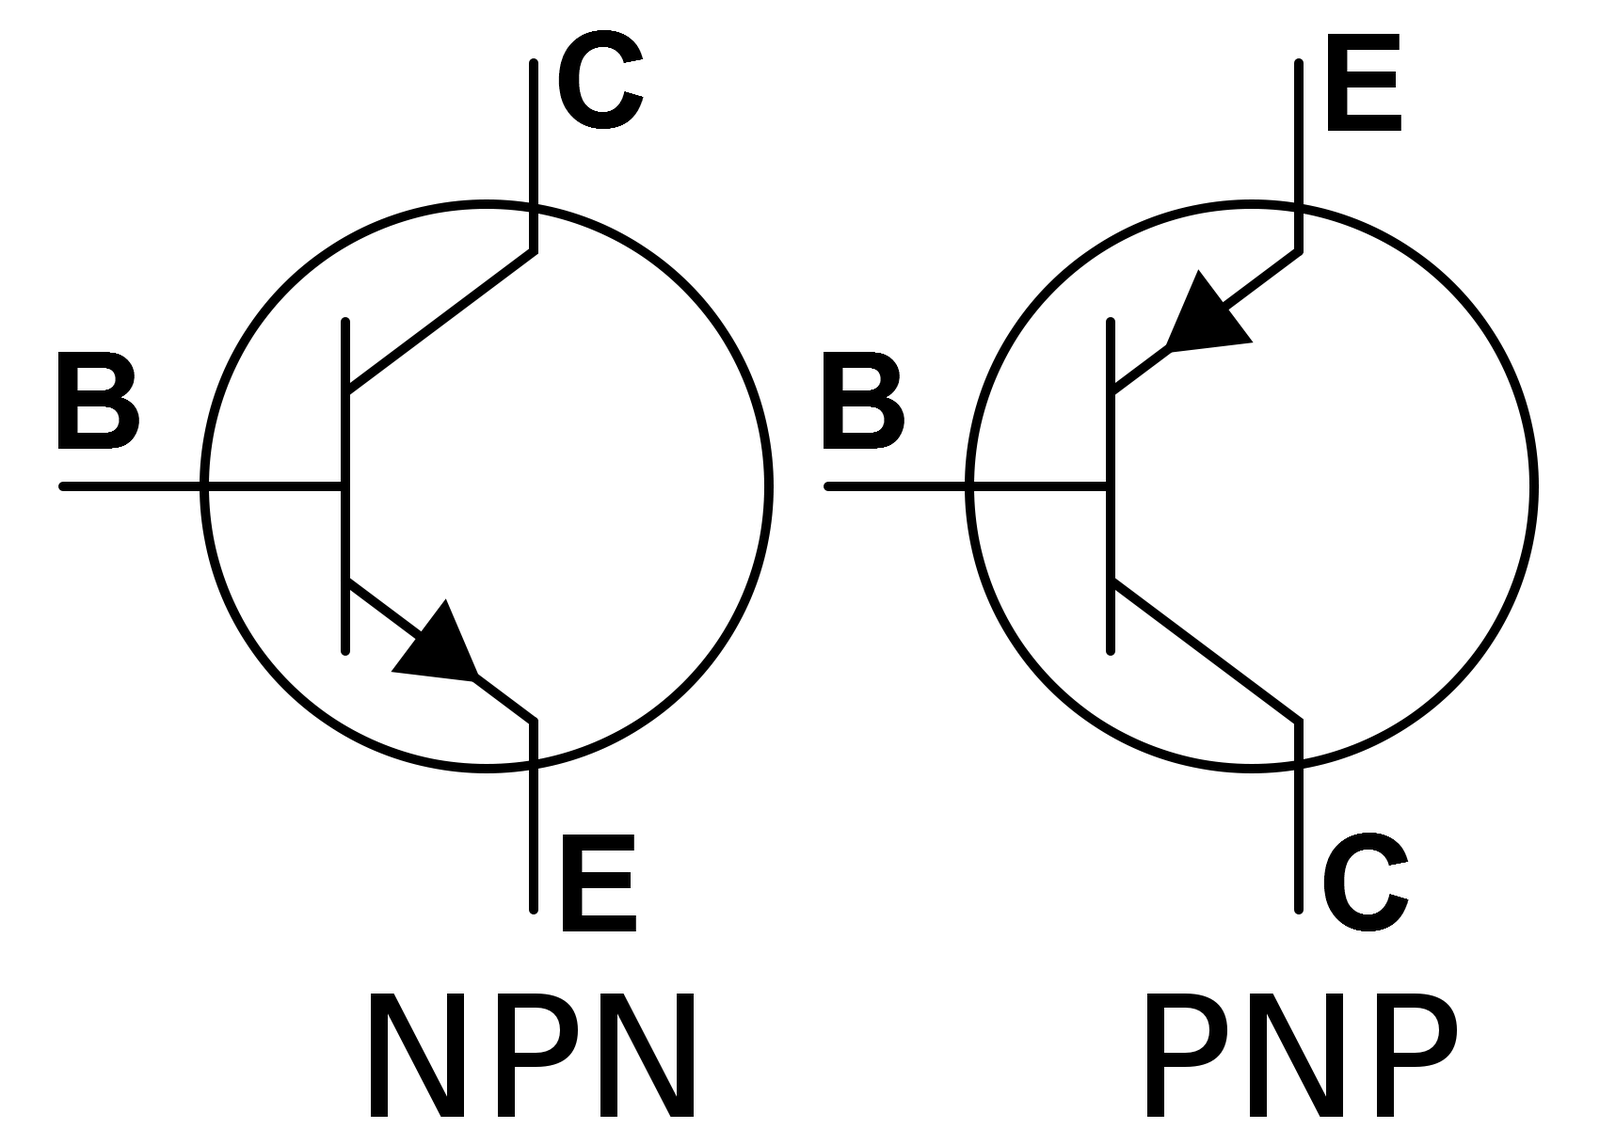
\includegraphics[width=4.5cm]{./bilder/Transistorer.png}
\end{textblock*}

\vissteduatt{Visste du att några kampvisor blivit reviderade i efterhand?}


\newpage

\subsection*{E-sektionens Kampvisa VII} 
\index[alfa]{E-sektionens Kampvisa VII}
\index[anfa]{E-sek på LTH} 
\songinfo{Mel: Anton aus Tirol \\ Text: Sebastian Elm (E12), Kewin Erichsen (E11)}

\begin{parse lines}[\noindent]{#1\\}
    ||: E-sek, E-sek, E-sek på LTH :||
    Vi slajdar in,
    med grym entré
    För det är vi som går på E!
    Vi lyser upp med bra manér,
    tänder gnistan inom er
    Det är eliten som ni ser!

    Är du för klen?
    De' e ingen kris
    Det fixar vi med dialys!
    När ni sedan vaknat opp,
    är vår spänning än på topp
    För det är vi som går på E!
    ||: E-sek, E-sek, E-sek på LTH :||

\end{parse lines}

\subsection*{E-sektionens Kampvisa VIII} 
\index[alfa]{E-sektionens Kampvisa VIII}
\index[anfa]{Alla vill höra våran sång} 
\songinfo{Mel: Anton aus Tirol \\ Sebastian Elm E12 \& Kewin Erichsen E11}

\begin{parse lines}[\noindent]{#1\\}
    Alla vill höra våran sång
    Därför vi sjunga gång på gång
    E-sek, här kommer E-sek
    Och alla andra, de kommer igång

\end{parse lines}

\vissteduatt{Visste du att kampvisa VII har en musikvideo på Youtube?}

\newpage


\subsection*{E-sektionens Kampvisa IX} 
\index[alfa]{E-sektionens Kampvisa IX}
\index[anfa]{Här kommer E-sektionen} 
\songinfo{Mel: Gärdebylåten}

\begin{parse lines}[\noindent]{#1\\}
    Här kommer E-sektionen
    Vackrast på hela jorden
    Tuborg i Edekvata, billigast i hela Lund
    Med vitt ska vi kiosken måla
    Sen för vår seger skåla
    Festa det gör vi bäst på E
    O alla får va me’
    \textbf{(Om man vill, Och det vill man!)}

\end{parse lines}


\subsection*{E-sektionens Kampvisa X} 
\index[alfa]{E-sektionens Kampvisa X}
\index[anfa]{Everywhere we go} 
%\songinfo{Mel: Gärdebylåten}

\begin{parse lines}[\noindent]{#1\\}

    Everywhere we go! \textit{Everywhere we go!}
    People wanna know! \textit{ People wanna know!}
    Who we are! \textit{Who we are!}
    So we tell them! \textit{So we tell them!}
    We are the E-sek! \textit{We are the E-sek!}
    Mighty mighty E-sek! \textit{Mighty mighty E-sek!}

    Oh ah å E-sek...

\end{parse lines}
\vissteduatt{Visste du att E-sektionen äger rättigheterna till F:s F och hyr ut \\det för den administrativa kostnaden att upprätthålla rättigheten?}
\newpage


\subsection*{E-sektionens Kampvisa XI} 
% \index[alfa]{E-sektionens Kampvisa X}
% \index[anfa]{Everywhere we go} 
\songinfo{Mel: \\Text:}

\begin{parse lines}[\noindent]{#1\\}
    

\end{parse lines}


\vissteduatt{Visste du att här kan man fylla i nya kampvisor?}
\newpage

\subsection*{E-sektionens Sexlåt} 
\index[alfa]{E-sektionens Sexlåt}
\index[anfa]{Sexets låt} 
\songinfo{Mel: När vindarna viskar mitt namn\\
Text: Sebastian Elm E12, Kewin Erichsen E11
}

\begin{parse lines}[\noindent]{#1\\}
    Jag var fångad i sexet, jag såg inget ljus
    In i dimman betygen försvann
    Jag jobbar och sliter, det finns ingen tid
    När FAN låg jag senast i fas

    Men de ger mig min styrka, ger mig sprit att förtära var natt
    En fyllecell, vårt mål, vi trivs bäst i vår vita kavaj!

    Vi mår va några jävla drägg, som går loss och dricker rent
    Men E6 styr upp spänningen

    //: När Gasquen den viskar vårt namn ://

\end{parse lines}

\vissteduatt{Visste du att "Gasquen" kan bytas till aktuell plats där sången
\\ framförs?}

\newpage

\subsection*{Medtekingenjören} 
\index[alfa]{Medtekingenjören}
\index[anfa]{Vi som botar alla sjuka} 
\songinfo{Mel: O hur saligt att få vandra
}

\begin{parse lines}[\noindent]{#1\\}
    Vi som botar alla sjuka
    Diagnos med hjälp av ultraljud
    Hårda delar liksom mjuka
    Vi placerar elektroder på din hud
    Och studerar sen effekten
    Tolkar diagrammets amplitud
    Om den påvisar defekter
    Med din hjärna så leker vi gud

    //: En röntgenbild, den gör mig vild
    och jag blir kär, får hjärtbesvär
    En blå pastill, och lite pill
    Får mig att tända till ://

    Gener kan manipuleras
    Ingenjörskonst på ett högre plan
    När vi dig har programmerat
    Blir du aldrig mer likadan
    Läkarna behandlar dig mot gaser
    Rektoskopi ja det slipper vi
    Istället leker vi med laser
    Och röntgen och MRI

\end{parse lines}

\vissteduatt{Visste du att  denna låt är skriven av MiT på KTH?}

\newpage

\begin{parse lines}[\noindent]{#1\\}
    Och läkarsprit - vår favorit
    Ja läkarsprit - mot hepatit
    Sälj läkarsprit - ge oss profit
    Mer läkarsprit

    Mer läkarsprit - fyll på ge hit
    Jag får aptit - av läkarsprit
    För läkarsprit - vår favorit
    Mer läkarsprit

\end{parse lines}

\begin{textblock*}{3cm}(0.2cm,5.1cm) % {width}(x, y)
    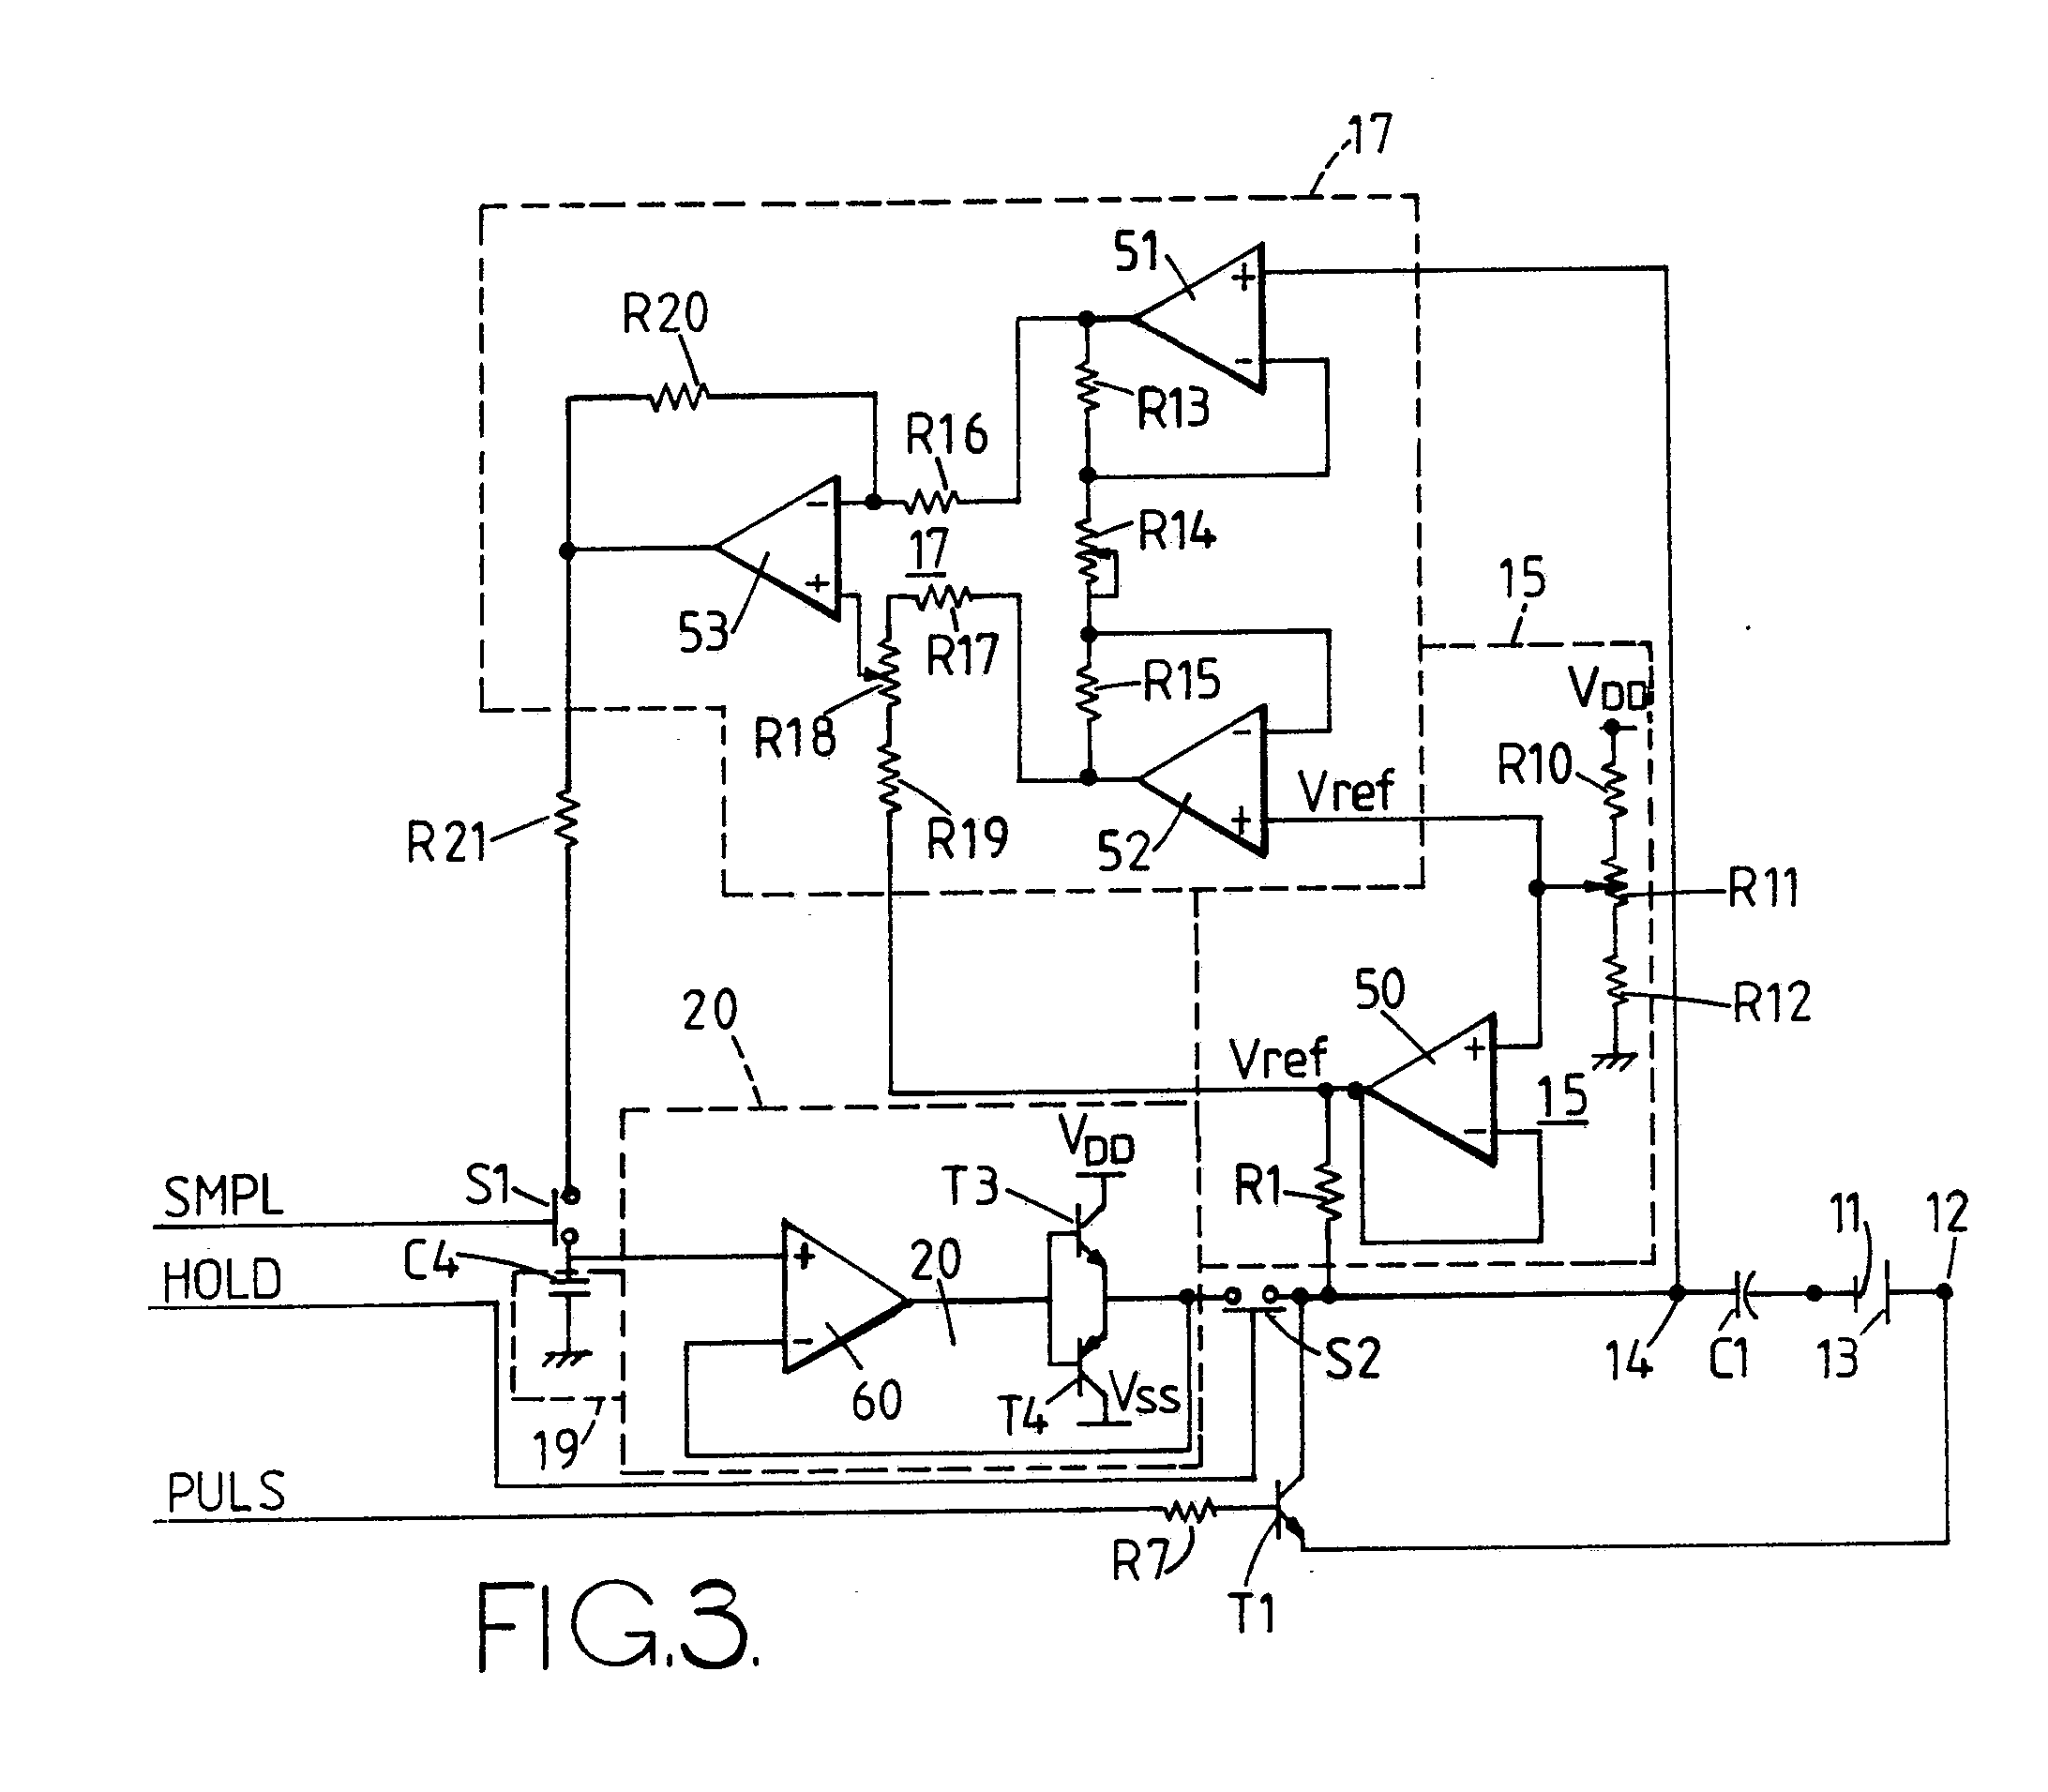
\includegraphics[width=9.9cm]{./bilder/PacemakerCircuit.png}
\end{textblock*}

\vissteduatt{Visste du att .... något mer om kth medtech eller BME? ELLER visste du att Pacemakern är en Lundauppfinning?}


\newpage


\subsection*{Mer jul} 
\index[alfa]{Mer jul}
\index[anfa]{Mer jul} 
\songinfo{Av: Falk Adolphson
}

\begin{parse lines}[\noindent]{#1\\}
    Jag är en lugn person med takt och ton
    måttfull och balanserad
    Jag är tyst och still och det ska mycket till 
    innan jag blir exalterad
    Men jag har en last som håller mig fast 
    i ett järngrepp varje vinter
    När året är slut och snön ligger djup 
    och slädarnas medar slinter

    Jag vill ha mer jul
    Ge mig mer jul
    Jag vill ha mer jul
    Ge mig mer jul
    Tusen stjärnor som tindrar,
    glitter så långt jag ser
    Av juleljus som glimmar,
    vill jag ha mer


\end{parse lines}

\newpage

\begin{parse lines}[\noindent]{#1\\}
    En show glöms bort om den bara visar opp 
    effekter som man knappast anar
    Så ge mig trettio grader kallt, tomtar överallt 
    och en skog av gröna granar
    Jag vill ha snötyngda hus, tusentals ljus, 
    kulörta kulor i drivor
    Bjällerklang som ackompanjemang 
    på alla julens skivor

    Jag vill ha mer jul…

    Ge mig en svårknäckt nöt, sötare gröt, 
    djupare dopp i grytan
    Glittrigare glim och grötigare rim 
    och mer Arne Weise i rutan
    Jag vill ha rymligare säck, segare knäck, 
    fetare fläsk från grisen
    Krimsigare krams, längre långdans 
    och raskare räv på isen

    Jag vill ha mer jul…

    Jag vill ha mer, mer
    Ge mig mer, mer
    Jag vill ha mer, mer
    Ge mig mer, mer

\end{parse lines}

\vissteduatt{Visste du att Mer Jul spelas årligen i Edekvata oavbrutet från och \\med Glöggillet fram till Julgillet är hållet?}

\newpage

\subsection*{Jag är liten nolla} 
\index[alfa]{Jag är liten nolla}
\index[anfa]{Jag är liten nolla}
\songinfo{Mel: Jag är fattig bonddräng\\
Text: JO Sivtoft, E94}

\begin{parse lines}[\noindent]{#1\\}
    Jag, en liten nolla, på Elektro jag går
    Dagar går och kommer, medan jag pluggar på
    Labbar, löddar, räknar, programmerar och lär, 
    Går på föreläsning, inför tentan jag svär

    Jag en fattig nolla, pasta lever jag på
    Och när fredan kommer till Edekvata jag gå
    Sen, när jag blitt livad, vill jag dansa, umgås
    Vila hos en flicka, vill jag också förstås

    Sen så kommer helgen, och då vill CSN
    Att jag pluggar satan, men då festar jag än
    40 timmars vecka, gäller inte för oss
    För oss teknologer, e de dubbelt förstås

    Så går hela veckan, varje läsperiod
    Åren går och kommer, men jag är vid gott mod
    Jag tar mina tentor, samlar på mig poäng, 
    Jag tar min examen, sen så blir jag utslängd

    Nu så väntar livet, som civilingenjör
    Nu så ska jag skörda, tjäna pengar som smör
    Men man jobbar sliter, si så där 40 år
    Till barn, familj o staten, alla pengarna går

    Så när dagen kommer, invid himmelens port, 
    Lite rädd och lessen, för de synder jag gjort
    Inte skattefuska, köra fort, supa loss
    Herren Gud i himlen, är väl missnöjd förstas

    Jag, vid pärleporten, blir nu eftertänksam
    De allra bästa åren, alltför snabbt de försvann
    Hade allt för bråttom, bort från de som var bäst
    Åren på Elektro, saknar jag allra mest

    Men då säger Herren: (civil) ingenjören, kom hit! 
    Jag har sett din strävan, och ditt eviga slit
    Därför, ingenjören, är du välkommen här
    Himmelens Elektro till du antagen är

    Jag som liten ängel, står så still inför Gud, 
    och sen klär han på mej en Elektrovit skrud
    Nu du, säger Herren, börjar vi om igen 
    Nu du, liten nolla, nu har du kommit hem

    Till dig liten nolla, sensmoralen den är
    Ha ej allt för bråttom, under tiden du lär
    Tids nog får du jobba, resten utav ditt liv
    Därför ta till vara, på studentlivets tid
\end{parse lines}

\vissteduatt{Visste du att... sjunges gärna på nollegasque(???)}


\newpage

\subsection*{Hacke Hackspett} 
\index[alfa]{Hacke Hackspett}
\index[anfa]{Hacke Hackspett}
\songinfo{Mel: Woody Woodpecker (Georg F. Tibbles, Ramey Idriss)\\
Text: Povel Ramel \& Georg Eliasson
}

\begin{parse lines}[\noindent]{#1\\}
     %\textit{Mitt namn är Hacke Hackspett, resande i Schweizerostar!}
    Hahahahaha! Hahahahaha! Hör på hackspettens melodi
    Hahahahaha! Hahahahaha! Med sin hackande harmoni!
    
    Han hackar sig fram
    ifrån stam till stam
    och bygger upp sitt höga C
    När du märker hans skratt,
    så ta på dig din hatt
    ty han är på jakt efter tre
    
    ||: Hahahahaha! Hahahahaha! 
    Har du hört en så’n retfull trall,
    Hahahahaha! Hahahahaha! 
    När du traskar bland gran och tall
    
    Om hans skönsång nu ej
    gör nå't intryck på dig,
    alla hackspettars hjärtan slår
    
    Hahahahaha! Hahahahaha! Varje gång det är sol och vår :||
\end{parse lines}

\vissteduatt{Visste du att Povel Ramel och hans glättiga gröngölingar spelade in\\
 låten på 78-varvare 23 september 1948?}


\newpage


%\input{kapitel/03-andra_sektioner.tex}

%\begin{center}
    \vspace*{1.5cm}
    {\fontsize{20}{20}\textbf{Klassiska visor}}\\
    \vspace{0.7cm}
    {\fontsize{12}{12}\textit{Om Taube själv får välja}}
\end{center}
\addtocwithheader{Klassiska visor}  % Add entry to TOC and set header
\thispagestyle{empty}
\noBackground

\newpage
\resetBackground

\subsection*{Måltidssången} 
\index[alfa]{Måltidssången}
\index[anfa]{Så lunka vi så småning om}
\songinfo{C. M. Bellman \\Fredmans sång N:o 21}

\begin{parse lines}[\noindent]{#1\\}
    Så lunka vi så småningom,
    från Bacchi buller och tumult
    när döden ropar: Granne, kom,
    ditt timglas är nu fullt
    Du gubbe fäll din krycka ner
    och du, du yngling lyd min lag:
    den skönsta nymf som åt dig ler
    inunder armen tag

    Tycker du att graven är för djup,
    nå välan, så tag dig då en sup,
    tag dig sen dito en, dito två, dito tre
    så dör du nöjdare

    Säg, är du nöjd, min granne säg?
    Så prisa värden nu till slut
    om vi har en och samma väg,
    så följoms åt... Drick ut!
    Men först med vinet rött och vitt,
    för vår värdinna bugom oss
    och halkom sen i graven fritt
    vid aftonstjärnans bloss

    Tycker du…
\end{parse lines}

\vissteduatt{Visste du att denna sjunges när alla fått sin varmrätt? %\\ När man sjunger "tycker du..." ska man kroka i arm med sina bordsgrannar    ?\\}

\newpage

\subsection*{Den blomstertid nu kommer} 
\index[alfa]{Den blomstertid nu kommer}
\index[anfa]{Den blomstertid nu kommer}

\begin{parse lines}[\noindent]{#1\\}
    Den blomstertid nu kommer
    med lust och fägring stor
    Nu nalkas ljuvlig sommar
    då gräs och gröda gror
    Den blida solen väcker
    allt det som varit dött
    Den allt med grönska täcker,
    och allt blir återfött

    De fagra blomsterängar
    och åkerns ädla säd,
    de rika örtesängar
    och alla gröna träd
    skall oss var dag påminna
    Guds godhets rikedom
    Låt oss den nåd besinna
    som räcker året om

\end{parse lines}

\newpage

\subsection*{Studentsången} 
\index[alfa]{Studentsången}
\index[anfa]{Sjung om studentens lyckliga dag}
\songinfo{Musik: Prins Gustaf\\
Text: Herman Sätherberg
}

\begin{parse lines}[\noindent]{#1\\}
    Sjung om studentens lyckliga dag,
    låtom oss fröjdas i ungdomens vår!
    Än klappar hjärtat med friska slag,
    och den ljusnande framtid är vår.
    ||: Inga stormar än
    i våra sinnen bo,
    hoppet är vår vän,
    och vi dess löften tro,
    när vi knyta förbund i den lund,
    där de härliga lagrarna gro!
    där de härliga lagrarna gro! :||
    Hurra!

\end{parse lines}

\newpage

\subsection*{O, gamla klang och jubeltid} 
\index[alfa]{O, gamla klang och jubeltid}
\index[anfa]{O, gamla klang och jubeltid}
\songinfo{Mel: O, alte Burschenherrlichkeit!
}

\begin{parse lines}[\noindent]{#1\\}
    O, gamla klang och jubeltid, 
    ditt minne skall förbliva
    och än åt livets bistra strid 
    ett rostigt skimmer giva!
    Snart tystnar allt vårt yra skämt,
    vår sång blir stum, vårt glam förstämt;
    o jerum, jerum, jerum,
    o, quae mutatio rerum!

    Var äro de, som kunde allt,
    blott ej sin ära svika,
    som voro män av äkta halt
    och världens herrar lika?
    De drogo bort från vin och sång
    till vardagslivets tråk och tvång;
    o, jerum, jerum, jerum,
    o, quae mutatio rerum!

    En tämjer forsens vilda fall,
    en annan ger oss papper,
    en idkar maskinistens kall,
    en mästrar volt så tapper,
    en ritar hus, en mäter mark,
    en blandar hop mixtur så stark;
    o, jerum, jerum, jerum,
    o, quae mutatio rerum!
\end{parse lines}

\vissteduatt{Visste du att denna sången sjungs när en sittning ska avlutas på\\ andra sektioner?}

\begin{parse lines}[\noindent]{#1\\}
    Men hjärtat i en sann student
    kan ingen tid förfrysa,
    den glädjeeld, som där han har tänt,
    hans hela liv skall lysa.
    Det gamla skalet brustit har,
    men kärnan finnes frisk dock kvar,
    och vad han än må mista,
    den skall dock aldrig brista!

    Så sluten, bröder, fast vår krets
    till glädjens värn och ära!
    Trots allt vi tryggt och väl tillfreds
    vår vänskap trohet svära.
    Lyft bägarn högt, och klinga, vän!
    De gamla gudar leva än
    bland skålar och pokaler,
    bland skålar och pokaler!
\end{parse lines}

\vissteduatt{Visste du att den tredje versen är LTH:s och KTH:s egna vers?}

\newpage

\subsection*{Längtan till landet} 
\index[alfa]{Längtan till landet}
\index[anfa]{Vintern rasat ut bland våra fjällar}
\songinfo{Musik: O. Lindblad\\ Text: H. Sätherberg}

\begin{parse lines}[\noindent]{#1\\}
    Vintern rasat ut bland våra fjällar,
    drivans blommor smälta ned och dö
    Himlen ler i vårens ljusa kvällar
    solen kysser liv i skog och sjö
    ||: Snart är sommar´n här! I purpurvågor,
    guldbelagda, azurskiftande
    ligga ägnarne i dagens lågor
    och i lunden dansa källorne :||

    Ja, jag kommer! Hälsen glada vindar
    ut till landet, ut till fåglarne,
    att jag älskar dem, till björk och lindar,
    sjö och berg, jag vill dem återse
    ||: Se dem än som i min bardoms stunder
    följa bäckens dans till klarnad sjö
    Trastens sång i furuskogens lunder,
    vattenfågelns lek kring fjärd och ö :||
\end{parse lines}

\vissteduatt{Visste du att sången sjungs av Lunds studentsångare 1:a maj varje\\år för att fira in våren?}

\newpage

\subsection*{Du gamla, du fria} 
\index[alfa]{Du gamla, du fria}
\index[anfa]{Du gamla, du fria}
\songinfo{Text: Richard Dybeck}

\begin{parse lines}[\noindent]{#1\\}
    Du gamla, du fria, du fjällhöga Nord
    du tysta, du glädjerika sköna
    Jag hälsar dig vänaste land uppå jord
    Din sol, din himmel, dina ängder gröna
    Din sol, din himmel, dina ängder gröna

    Du tronar på minnen från fornstora dar
    då ärat ditt namn flög över jorden
    Jag vet att du är och du blir vad du var
    Ja, jag vill leva, jag vill dö i Norden
    Ja, jag vill leva, jag vill dö i Norden
\end{parse lines}

% \vissteduatt{visste du att...En händelse som enligt historien bidrog till \\
% att sången började få status som nationalsång var vid en promotionsmiddag \\
% vid Lunds Universitet våren 1893, då Kung Oscar II ställde sig upp när sången framfördes.}

\vissteduatt{Visste du att enligt historien fick sången status som nationalsång\\efter en promotionsmiddag vid Lunds Universistet 1893, när\\Kung Oscar II reste sig under framförandet?}

\newpage

\subsection*{Brevet från kolonien} 
\index[alfa]{Brevet från kolonien}
\index[anfa]{Brevet från kolonien}
\songinfo{Cornelis Vreeswijk}

\colorbox{yellow}{OSÄKER PÅ DENNA}

\begin{parse lines}[\noindent]{#1\\}
    Hejsan morsan, hejsan stabben
    Här är brev från älsklingsgrabben
    Vi har kul på kolonien
    Vi bor tjugoåtta gangstergrabbar i en

    Stor barack med massa sängar
    Kan ni skicka mera pengar?
    För det vore en god gärning
    Jag har spelat bort vartenda dugg på tärning

    Här är roligt vill jag lova
    Fastän lite svårt att sova
    Killen som har sängen över mig
    Han vaknar inte han när han behöver, nej

    Jag har tappat två framtänder
    För jag skulle gå på händer
    När vi lattjade charader
    Så när morsan nu får se mig får hon spader

    Ute i skogen finns baciller
    Men min kompis han har piller
    Som han köpt utav en ful typ
    Och om man äter dem blir man en jättekul typ

    Våran fröken är försvunnen
    Hon har dränkt sig uti brunnen
    För en morgon blev hon galen
    När vi släppte ut en huggorm i matsalen

    Men jag är inte, rädd för spöken
    För min kompis han har kröken
    Som han gjort utav potatis
    Och som han säljer i baracken nästan gratis

    Föreståndaren han har farit
    Han blir aldrig var han varit
    För polisen kom och tog hand
    Om honom förra veckan när vi lekte skogsbrand

    Ute i skogen finns det rådjur
    I baracken finns det smådjur
    Och min bäste kompis Tage
    Han har en liten fickkniv inuti sin mage

    Honom ska de operera
    Ja, nu vet jag inge mera
    Kram och kyss och hjärtligt tack sen
    Men nu ska vi ut och bränna grannbaracken
\end{parse lines}

\vissteduatt{visste du att...}

\newpage

\subsection*{Skånska slott och herresäten} 
\index[alfa]{Skånska slott och herresäten}
\index[anfa]{Skånska slott och herresäten}
\songinfo{Text: Hjalmar Gullberg, Bengt Hjelmqvist,
Sång: Edvard Persson}

\colorbox{yellow}{OSÄKER PÅ DENNA}

\begin{parse lines}[\noindent]{#1\\}
    På himmelen vandra sol, stjärnor och måne
    Och kasta sitt fagraste ljus över Skåne
    På höga och låga, på stort och på smått
    På statarens koja och ädlingens slott

    Se månstrålen in genom blyrutan faller
    Och tecknar på golvet det järnsmidda galler
    Stolts jungfrun hon drömmer i majnattens ljus
    Att friare komma till Glimmingehus

    På utflykt till Bokskogen Malmöbon glor upp
    Mot raden av strålande fönster på Torup
    Att smaka på kaka som bakats på spett
    Dig ber hennes nåd, friherrinnan Coyet

    Där rådjuren skymta bak'vitgråa stammar
    Man ser Toppela'gård med broar och dammar
    Systemet på sprit och på skatterna sta'n
    Där lurar belåtet fiskalen Aschan

    Med port genom huset och gamla kanaler
    Lyss Skabersjö ännu till jaktens signaler
    Själv kungen i nåder far dit från sitt slott
    Och skjuter fasaner med grevarna Thott

    Och därefter hälsar han på baron Trolle
    Och jagar och spelar sin sans och sin nolle
    Allt medan baronens gemål
    Plockar gräs åt rastupp och rashöna på Trollenäs
\end{parse lines}

\vissteduatt{visste du att...}


\newpage

\subsection*{Kungssången} 
\index[alfa]{Kungssången}
\index[anfa]{Ur svenska hjärtans djup en gång}
\songinfo{Musik: Otto Lindblad Text: C.V.A Strandberg}

\colorbox{yellow}{OSÄKER PÅ DENNA}

\begin{parse lines}[\noindent]{#1\\}
    Ur svenska hjärtans djup en gång en samfälld och en enkel sång,
    som går till kungen fram! Var honom trofast, och hans ätt,
    gör kronan på hans hjässa lätt, och all din tro till honom sätt, 
    du folk av frejdad stam! O konung, folkets majestät är även ditt: 
    beskärma det och värna det från fall! Stå oss all världens härar mot, 
    vi blinka ej för deras hot: vi lägga dem inför din fot - en kunglig fotapall. 
    Du himlens Herre, med oss var, som förr Du med oss varit har, 
    och liva på vår strand det gamla lynnets art igen hos sveakungen och hans män. 
    Och låt Din ande vila än utöver nordanland!
\end{parse lines}

\vissteduatt{visste du att vissa studenter inleder alla sittningar med denna...}


\newpage




% \input{kapitel/05-skånska_visor.tex}

% \begin{center}
    \vspace*{1.5cm}
    {\fontsize{20}{20}\textbf{Teknologvisor}}\\
    \vspace{0.7cm}
    {\fontsize{12}{12}\textit{Om teknologen själv får välja}}
\end{center}
\addtocwithheader{Teknologvisor}  % Add entry to TOC and set header\noBackground
\noBackground

\newpage
\resetBackground


\subsection*{Porthos visa} 
\index[alfa]{Porthos visa}
\index[anfa]{Jag vill börja gasqua!}
\songinfo{Mel: You can't get a man with a gun \\(ur Annie get your gun)\\Text: T Andrén}
\colorbox{yellow}{Vi måste bestämma hur texten ska vara. Samma som i förra boken \\eller ska vi följa vad vi hittar i andra böcker eller online?}

\begin{parse lines}[\noindent]{#1\\}
    Jag vill börja gasqua!
    Var fan är min flaska?
    Vem i helvete stal min butelj?
    Skall mej törsten betvinga?
    En TT börja svinga?
    Nej för fan bara blunda och svälj!
    Vilken smörja!
    Får jag spörja?
    Vem för fan tror att jag är en älg?
    Till England vi rider,
    och sedan vad det lider,
    träffar vi välan på någon PUB
    Och där skall vi festa!
    Blott dricka utav det bästa
    utav Whiskey och Portvin
    Jag tänker gå hårt in
    för att prova på rubb och stubb
    Rubb och stubb…
\end{parse lines}

\vissteduatt{Visste du att om den sista "stubb" sjunges så måste låten upprepas...}

% \newpage


\subsection*{En komplex värld} 
\index[alfa]{En komplex värld}
\index[anfa]{Alla jävla bevis}
\songinfo{Mel: En helt ny värld (ur Aladdin)\\
Text: Ellinor Persson F07 och Andreas Tågerud F06
}

\begin{parse lines}[\noindent]{#1\\}
    Alla jävla bevis
    inses lätt som en övning.
    Javakursen en prövning
    för min bristande logik.

    Ska man komma ihåg
    alla formler i huvet?
    Formelsamlingen, du vet,
    säger inget om det här!

    En komplex värld
    Vad fan betyder bijektiv?
    Ingenting stämmer här, där allt jag lär,
    blir glömt snart efter tentan.
    Hur ska det gå?
    Och det är bara vecka två...
    Känner en underton av aggression
    mot allt Sven Spanne skrivit i sin bok

    (Jag kan transponera den...)
\end{parse lines}

\newpage

\begin{parse lines}[\noindent]{#1\\}
    Jag kan lära dig C
    Matematiska under
    Oförglömliga stunder
    när vi tentar mekanik

    Det ska nog gå!
    Det sa din mamma med igår
    All tid tillvaratas, jag är i fas,
    och bor i mattehuset.
    Nu är jag lärd!
    Till denna svåra ekvation
    jag på frekvenssidan en lösning fann,
    den låg där i en helt ny värld: Laplace!
\end{parse lines}

\subsection*{Enhetsvisan / SI - Système International d'Unités} 
\index[alfa]{Enhetsvisan / SI - Système International d'Unités}
\index[anfa]{1, 2, 75, 6, 7}
\songinfo{Mel: Studentsången}

\begin{parse lines}[\noindent]{#1\\}
    W kg m Wb s
    Ω m T A rad
    cd Sv N s
    Ω A m lx dB
    °C W/m²
    J/kg H V C
    kg/m3 mol
    m/s²
    m/s²
    F !
\end{parse lines}

\vissteduatt{Visste du att SI-låttexten finns i TeFyma?}

\newpage

\subsection*{Man ska ha matlab} 
\index[alfa]{Man ska ha matlab}
\index[anfa]{Man ska ha matlab}
\songinfo{Mel: Man ska ha husvagn}

\begin{parse lines}[\noindent]{#1\\}
    Jag har prövat nästan allt som finns att pröva på
    Beta, kulram, räknesticka, tärning eller så
    Jag har kalkylerat på de konstigaste sätt
    och nu så har jag kommit på hur man ska räkna rätt

    Man ska ha MATLAB - då är kalkylen redan klar
    Man ska ha MATLAB - det har jag sett att andra har
    Man ska ha MATLAB - det är min livsfilosofi
    Man ska ha MATLAB - för då blir man fri

    I många år så var jag inte alls så särskilt lärd
    Jag visste ej vad som vänta' mig i denna stora värld
    Men sen kom jag till LTH, och ända sedan dess
    så har jag funnit livets stora lyxdelikatess

    Man ska ha MATLAB - så man slipper tänka alls
    Man ska ha MATLAB - ja, då går allting som en vals
    Man ska ha MATLAB - det bygger på nån slags logik
    Man ska ha MATLAB - för då blir man rik

    5 minuter mekanik och 5 minuter statfys
    5 minuter plottande och 5 minuter analys
    5 minuter fråga phadder, 5 minuter stopp
    5 minuter tänka själv och sen så ger man opp
\end{parse lines}

\vissteduatt{Vad kom först MATLAB eller Maple?}

\newpage

\begin{parse lines}[\noindent]{#1\\}
    Man ska ha MATLAB - och datasalens friska luft
    Man ska ha MATLAB - det tycker tjejerna är tufft
    Man ska ha MATLAB - när ryssen kommer med sitt MIG
    Man ska ha MATLAB - då vinner man i krig!
\end{parse lines}

\vissteduatt{visste du att}

\newpage

\subsection*{Teknologvisa} 
\index[alfa]{Teknologvisa}
\index[anfa]{Jag är teknolog och helt OK}
\songinfo{Mel: The Lumberjack Song (Monty Python)\\ Sångarstriden 1982\\ Kursivt sjunges av sångförman}

\noindent\textit{Jag är teknolog och helt OK\\
Jag jobbar hårt och jag roar mig}\\\\
\noindent Han är teknolog och helt OK\\
Han jobbar hårt och han roar sig\\\\
\noindent\textit{Teknik är ball\\
Jag kan Pascal\\
Till Lophtet vill jag gå\\
Där träffas alla vänner\\
som är från LTH}\\\\
\noindent Teknik är ball\\
Han kan Pascal\\
Till Lophtet vill han gå\\
Där träffas alla vänner\\
som är från LTH\\\\
\noindent För han är teknolog och helt OK\\
Han jobbar hårt och han roar sig\\\\

\vissteduatt{Visste du att "Han" kan eneklt bytas ut mot "Hon" eller "Hen"!}

\newpage

\noindent\textit{Min mattebok \\
den gör mig klok\\
Jag läser kärnfysik\\
Jag går på föreläsning\\
och älskar juridik}\\\\
\noindent Hans mattebok\\
den gör han klok\\
Han läser kärnfysik\\
Han går på föreläsning\\
och älskar juridik???\\\\
\noindent Men han är teknolog och helt OK\\
Han jobbar hårt och han roar sig\\\\
\noindent\textit{Som ekonom jag blir fantom\\
Konkurser gör mig säll\\
Till flickor blankt jag nekar\\
Jag älskar en tabell}\\\\
\noindent Som ekonom han blir fantom???\\
konkurser...\\
Nää, BUU!!\\\\
\noindent Men han är teknolog och helt OK\\
Han jobbar hårt och han roar sig\\


\newpage

\subsection*{Flerdimensionell ångest} 
\index[alfa]{Flerdimensionell ångest}
\index[anfa]{Flerdimensionell ångest}
\songinfo{Mel: Härjarevisan\\
Text: Daniel Milve F11}

\begin{parse lines}[\noindent]{#1\\}
    Jag har aldrig sett mig själv som välkalkylerad
    Riktningsderivata gör min hjärna punkterad
    Man borde börjat lyssna redan
    Typ när nollningen tog stopp
    Än har jag ingen aning om vad Green’s formel säger
    Dock vet jag klart och tydligt vad de dryga förtäljer:
    Skillnaden mellan kurs och fest är 
    Kurser kan man göra om!

    Men så nu ska vi ut och tenta
    Statens små bidrag hämta
    Differentialer, integral och vektoranalys (i planet!)
    Fem timmar med hårda tag och
    Nu änteligen lär jag
    Kunna dra nån nytta av vad Månsson sade vecka två!
\end{parse lines}

\vissteduatt{Visste du att...}


\newpage


\subsection*{O, hemska labb} 
\index[alfa]{O, hemska labb}
\index[anfa]{O, hemska labb}
\songinfo{Mel: O, helga natt}

\colorbox{orange}{OSÄKER PÅ DENNA}

\begin{parse lines}[\noindent]{#1\\}
    O, hemska labb, o grymma kval imorgon
    Här sitter jag och förstår ingenting
    Hela mitt inre är fyllt utav ett motstånd
    emot eländig elektrisk mätteknik
    Jag skulle nog behöva lite ledning,
    här räcker inte min kapacitans
    Kondensatorer och felvända dioder
    O, hemska labb nu vill jag koppla af
    O, hemska labb ty detta blir min graf

    O, hemska labb, o grymma kval imorgon
    Här sitter jag och förstår ingenting
    Hela programmet är fyllt utav funktioner
    som innehåller en himla massa fel
    Pekare som inte har nån riktning,
    oändliga loopar, oj vad jag blir sträng!
    Åh, kompilera, hur ska det här fungera?
    O, hemska labb, nu vill jag logga ut
    O, hemska labb, ty detta blir mitt slut
\end{parse lines}

\vissteduatt{Visste du att...}


\newpage


\subsection*{Tenta efter jul} 
\index[alfa]{Tenta efter jul}
\index[anfa]{Tenta efter jul}
\songinfo{Mel: Mössens julafton\\
Skriva om att D-sektionen vinnande bordvisa (SåS enligt sångarkiv)}

\colorbox{yellow}{OSÄKER PÅ DENNA}

\begin{parse lines}[\noindent]{#1\\}
    När julen börjar närmas
    och man vill koppla av
    Så kommer tentaplugget
    här och ställer sina krav

    Jag börjar kompromissa
    gör julrimmen i C
    Försöker strukturera
    pluggar fram till klockan tre

    Programmering lin-jär algebra
    Endim å reglerteknik är ingenting att ha
    Tenta efter nyår är ju trist
    Men skippar man för många ja då blir man alkolist

    Skål! 
\end{parse lines}

\vissteduatt{Visste du att...}


\newpage




% \input{kapitel/07-ölvisor.tex}

% \begin{center}
    \vspace*{1.5cm}
    {\fontsize{20}{20}\textbf{Vinvisor}}\\
    \vspace{0.7cm}
    {\fontsize{12}{12}\textit{Om den nytvättade vita skjortan själv får välja}}
\end{center}
\addtocwithheader{Vinvisor}  % Add entry to TOC and set header\noBackground
\noBackground

\newpage
\resetBackground

\subsection*{\colorbox{red}{Tar bort: Lovsången till kvinnan}} 
% \index[alfa]{Öl, öl, öl i glas}
% \index[anfa]{Öl, öl, öl i glas}
% \songinfo{Mel: Row your boat}

\begin{parse lines}[\noindent]{#1\\}
    tas bort
\end{parse lines}

\vissteduatt{Visste du att...}

\newpage

\subsection*{Feta fransyskor} 
\index[alfa]{Feta fransyskor}
\index[anfa]{Feta fransyskor}
\songinfo{Mel: Militärmarsch av Schubert\\
K-sektionen Sångarstriden 1985}

\begin{parse lines}[\noindent]{#1\\}
    Feta fransyskor som svettas om fötterna,
    de trampar druvor
    som sedan ska jäsas till vin
    Transpirationen viktig é,
    ty den ge'
    fin bouquet
    Vårtor och svampar följer me'
    men vad gör väl de'?

    För vi vill ha vin,
    vill ha vin,
    vill ha mera vin,
    även om följderna blir
    att vi må lida pin
    Flaskan och glaset gått i sin
    Hit med vin, mera vin!
    Tror ni att vi är fyllesvin?
    {\Large Ja!} (Fast större!)
\end{parse lines}

\vissteduatt{Visste du att...}


\newpage


\subsection*{Lyft ditt välförsedda glas} 
\index[alfa]{Lyft ditt välförsedda glas}
\index[anfa]{Lyft ditt välförsedda glas}
\songinfo{Mel: Ding dong merrily on high}

\begin{parse lines}[\noindent]{#1\\}
    Lyft ditt välförsedda glas
    Det är en härlig börda
    Nu har grabbarna kalas
    Ve segern snart skall skörda
    //: Ding dingedingeding dingedingeding
    dingedingeding dong dong
    Imorgon är det lördag ://

    Sätt nu glaset till din mun
    Se döden på dig väntar
    Nu har grabbarna kalas
    Hör liemannen flämtar
    //: Ding dingedingeding dingedingeding
    dingedingeding dong dong
    Begravningsklockor klämtar ://
\end{parse lines}

\vissteduatt{Visste du att...}


\newpage


\subsection*{Bordeaux, bordeaux} 
\index[alfa]{Bordeaux, bordeaux}
\index[anfa]{Jag minns än idag hur min fader}
\songinfo{Mel: I sommarens soliga dagar}

\begin{parse lines}[\noindent]{#1\\}
    Jag minns än idag hur min fader
    kom hem ifrån staden så glader
    och rada' upp flaskor i rader
    och sade nöjd som så:
    "Bordeaux, Bordeaux!"

    Han drack ett glas, kom i extas,
    och sedan blev det stort kalas
    Och vi små glin, ja vi drack vin
    som första klassens fyllesvin
    Och vi dansade runt där på borden
    och skrek så vi blev blå:
    "Bordeaux, Bordeaux!"
\end{parse lines}

\vissteduatt{Visste du att...}


\newpage


\subsection*{Vinbröder} 
\index[alfa]{Vinbröder}
\index[anfa]{Två bröder, Jan-Ove och Hadar}
\songinfo{Mel: I sommarens soliga dagar}

\begin{parse lines}[\noindent]{#1\\}
    Två bröder, Jan-Ove och Hadar,
    de plockade fram sina spadar,
    och grävde en grop bakom huset.
    De hade en idé:
    Vaddå, vaddå?
    Jo, priset på 
    Kir och Bordeaux,
    är högt men om man gjorde så,
    att man i gropen lade ner,
    två kilo jäst och en back MER,
    så skulle det nog vara möjligt
    att producera vin i detta hål! Skål!
\end{parse lines}

\vissteduatt{Visste du att...}


\newpage


\subsection*{Karnaugh, karnaugh} 
\index[alfa]{Karnaugh, karnaugh}
\index[anfa]{Karnaugh, karnaugh}
\songinfo{Mel: I sommarens soliga dagar}

\begin{parse lines}[\noindent]{#1\\}
    Jag minns än i dag hur min fader
    kom hem i från labbet så glader
    och rada' upp bitar i rader
    och sade glad som så:
    Karnaugh, Karnaugh!

    Å ett å noll \& noll å ett 
    å booleska uttryck det är fett!
    Med ett å noll \& noll å ett,
    ska du nu se att det blir rätt,
    Men vi felsökte våra signaler,
    och det blev fel ändå
    Karnaugh, Karnaugh!
\end{parse lines}

\vissteduatt{Visste du att...}


\newpage


\subsection*{I sommarens soliga dagar} 
\index[alfa]{I sommarens soliga dagar}
\index[anfa]{I sommarens soliga dagar}
\songinfo{Mel: I sommarens soliga dagar\\
Text: Anders Nilsson $\pi$03 och Björn Carlin $\pi$02}

\begin{parse lines}[\noindent]{#1\\}
    I sommarens soliga dagar
    Kall rå fisk till alla vi lagar
    Och sätter oss ute i hagar
    Där maten härsken står
    Bakteriehärd av solen närd
    Den höjer högt sitt blanka svärd
    Men mot dess hot vi funnit bot 
    Vi sätter spritens krafter mot
    För spriten kan döda det mesta
    Vi hälsan återfår, Gutår! Gutår!
\end{parse lines}

\vissteduatt{Visste du att...}


\newpage


\subsection*{Kosmetisk visa} 
\index[alfa]{Kosmetisk visa}
\index[anfa]{Du behöver inte ha nåt läppstift alls}
\songinfo{Mel: She’ll be Coming ‘Round the Mountain\\
Lundakarnevalen 2002}

\begin{parse lines}[\noindent]{#1\\}
    Du behöver inte ha nåt läppstift alls,
    du behöver inte ha nåt läppstift alls,
    för när vinet börjar flöda,
    färgas läpparna ju röda,
    liksom tungan, hakan, skjortan och din hals!
\end{parse lines}

\vissteduatt{Visste du att...}


\newpage


\subsection*{Magnumflaskan Åkesson} 
\index[alfa]{Magnumflaskan Åkesson}
\index[anfa]{Magnumflaskan Åkesson}
\songinfo{Mel: Teddybjörnen Fredriksson\\
Lundakarnevalen 2010}

\begin{parse lines}[\noindent]{#1\\}
    För längesen, när jag fyllde 15 år
    fick jag en flaska av min mor
    Hon sa "Mitt barn, dela den med vännerna
    För den är faktiskt ganska stor."

    Magnumflaskan Åkesson,
    du var så stor och tung
    Jag gick runt med dig i hand,
    och i Dalby var jag kung

    Magnumflaskan Åkesson,
    din kork försvann i skyn
    Men jag drack dig bara själv
    Och kräktes i hela byn
\end{parse lines}

\vissteduatt{Visste du att...}


\newpage


\subsection*{\colorbox{orange}{Korkskruvens visa}} 
% \index[alfa]{Magnumflaskan Åkesson}
% \index[anfa]{Magnumflaskan Åkesson}
\songinfo{Mel: Nu har vi ljus}

\begin{parse lines}[\noindent]{#1\\}
    TA BORT???

    Nu har vi rus här i vårt hus
    Korken är borta hopptralalala
    Doften är ljuv, jag är en skruv,
    jag är en skruv.

    Jag kan inte öppna bag-in-boxen,
    jag kan inte öppna bag-in-boxen

    Lalalala lalalala lalalalala lala
\end{parse lines}

\vissteduatt{Visste du att...}


\newpage


\subsection*{Dance macabre} 
\index[alfa]{Dance macabre}
\index[anfa]{runt våran stuga, små djävlar sluga}
\songinfo{Mel: Vårvindar friska}

\begin{parse lines}[\noindent]{#1\\}
    Runt våran stuga, små djävlar sluga
    tassa så tyst med bockfot och svans
    Varulvar yla, isande kyla
    sveper i dimman, fantygets dans
    Bäva, o broder, lyssna och hör
    vrålen från gast, som osalig dör
    Satan han skrattar,
    flaskan han fattar,
    super tills dagen gryr.

    Gastar och spöken
    skymta i köken,
    dödingar släpa ruttnande lik
    Benrangel skramla,
    spökhänder famla,
    kväva din strupes rosslande skrik
    Helvetes alla fasor släpps loss
    Fan rider här med hela sin tross
    Göm dig i stugan,
    du har fått flugan
    Dille det blir din lott

\end{parse lines}

\vissteduatt{Visste du att man viskar hela låten fram till \\ "Helvetets alla fasor..." då tar man i för Kung och fosterland?}


\newpage




% \begin{center}
    \vspace*{1.5cm}
    {\fontsize{20}{20}\textbf{Snapsvisor}}\\
    \vspace{0.7cm}
    {\fontsize{12}{12}\textit{Om helan själv får välja}}
\end{center}
\addtocwithheader{Snapsvisor}  % Add entry to TOC and set header\noBackground
\noBackground

\newpage
\resetBackground

\begin{textblock*}{3cm}(0.0cm,0.2cm) % {width}(x, y)
    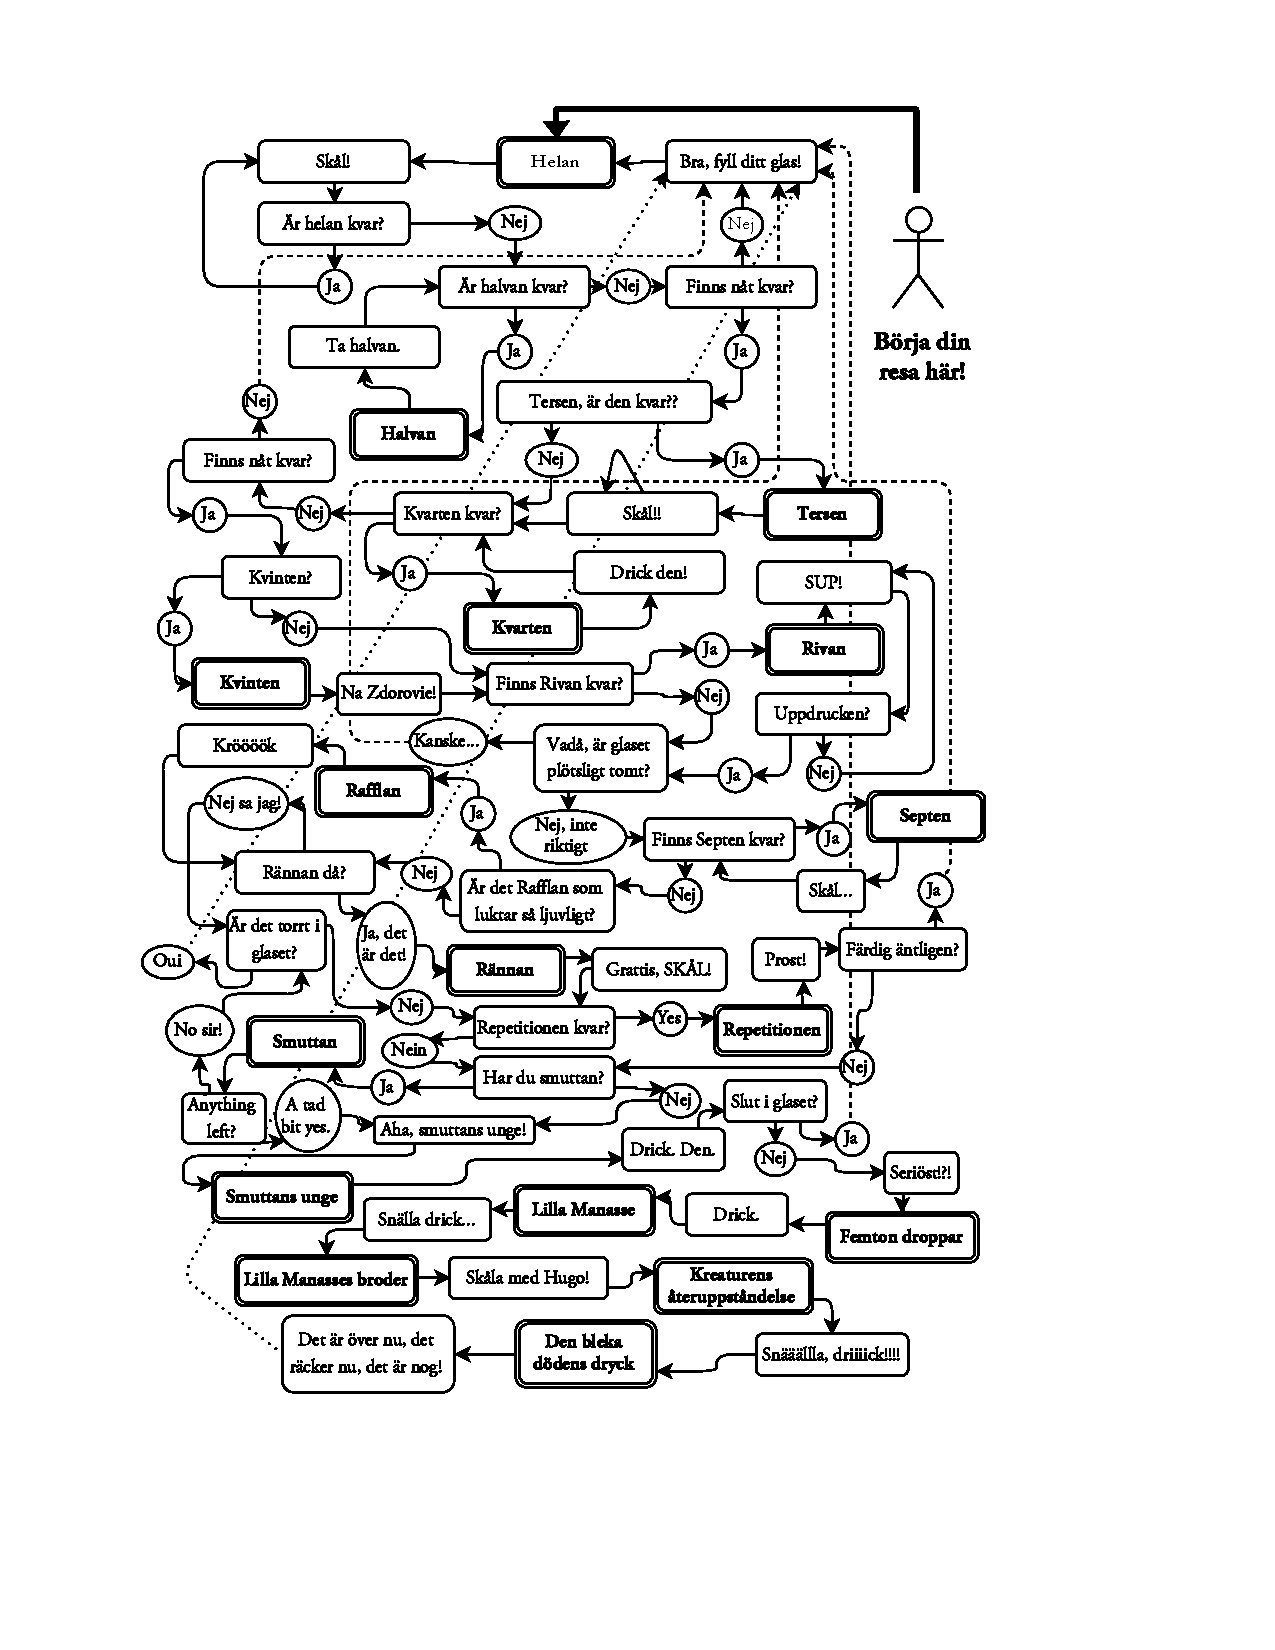
\includegraphics[width=12cm]{./bilder/SupSchema_FINAL_2.pdf}
\end{textblock*}

osynlig text

\vissteduatt{Har du kommit fram till "Den bleka dödens dryck" har du varit \\mycket sparsam. Bra jobbat!}

\newpage

\subsection*{Törsten rasar} 
\index[alfa]{Törsten rasar}
\index[anfa]{Törsten rasar uti våra strupar}
\songinfo{Mel: Längtan till landet}

\begin{parse lines}[\noindent]{#1\\}
    Törsten rasar uti våra strupar,
    tungan hänger torr och styv och stel
    Men snart vankas stora, kalla supar,
    var och en får sin beskärda del
    Snapsen kommer, den vi vilja tömma,
    denna nektar lik Olympens saft,
    kommer oss att våra sorger glömma
    Snapsen skänker hälsa, liv och kraft

    Fordom odlade man vindruvsranka,
    av vars frukt man gjorde ädelt vin
    Nu man pressar saften ur en planka,
    doftande av äkta terpentin
    Höj din bägare, O, Broder, yster,
    och låt svenska skogen glida kall,
    ner för strupen och om sen det dig lyster,
    låt oss supa opp en liten tall
\end{parse lines}

\vissteduatt{Visste du att funktionärsposten macapär infördes efter att sektionen\\köpt sin första Mac?}

\newpage

\begin{parse lines}[\noindent]{#1\\}
    Helan tänder helig eld i själen,
    halvan rosar livet som en sky
    Tersen känns från hjässan ner i hälen,
    kvarten gör oss till en mänska ny
    Låt oss skåla med varann, go' vänner,
    skål för våran levnads glada lopp,
    törstens eld på nytt i strupen bränner
    Leve livet! Skål och botten opp!

\end{parse lines}

\subsection*{Helan går} 
\index[alfa]{Helan går}
\index[anfa]{Helan går}
\songinfo{Kursivt sjunges av sångförman}

\begingroup
\itshape
\noindent Det satt en liten fågel på en gren\\
\noindent och sjöng i furuskogen\\
\noindent Han hade sjungit hela dagen lång,\\
\noindent men dock ej sjungit nog än\\
\noindent Men vad sjöng den lilla fågeln då?\\
\noindent Jo! Han sjöng:\\
\endgroup

\begin{parse lines}[\noindent]{#1\\}
    Helan går,
    sjung hopp faderallan lallan lej,
    Helan går,
    sjung hopp faderallan lej.
    Och den som inte helan tar,
    han heller inte halvan får
    Helan går,
    sjung hopp faderallan lej
\end{parse lines}

\newpage

\subsection*{Samling vid pumpen} 
\index[alfa]{Samling vid pumpen}
\index[anfa]{Samling vid pumpen}
\songinfo{Mel: Hujedamej sån’t barn han var}

\begin{parse lines}[\noindent]{#1\\}
    Samling nu vid pumpen 
    alla ni som dricker vatten 
    Vi som dricker brännvin 
    vi höjer våra glas 
    Vatten ska man ha 
    när man ska vattna i rabatten 
    Brännvin ska man ha 
    när man e på kalas!

\end{parse lines}


\subsection*{Inre dialog} 
\index[alfa]{Inre dialog}
\index[anfa]{Jag vill inte ha}
\songinfo{Mel: An der Schönen Blauen Donau\\
Kursivt sjunges av sångförman}

\textit{Jag vill inte ha} \hfill En nubbe till! \hspace*{15pt} \\
\textit{Jag  mår inte bra} \hfill En nubbe till! \hspace*{15pt} \\
\textit{Om ni ger mig mer} \hfill En nubbe till! \hspace*{15pt} \\
\textit{ser jag er som fler} \hfill En nubbe till! \hspace*{15pt} \\
\textit{Min mage är sjuk} \hfill En nubbe till! \hspace*{15pt} \\
\textit{Min hjärna är mjuk} \hfill En nubbe till! \hspace*{15pt} \\
\\
\textit{Jag kan inte tääänkaaa så braaa}\\
\textit{så jag får väl nubben ta} \hfill HURRA! \hspace*{37pt} 

\vissteduatt{Visste du att rummet Pump heter Pump eftersom fontänens pump\\tidigare stod i det rummet?}

\newpage


\subsection*{Tänk om jag hade lilla nubben} 
\index[alfa]{Tänk om jag hade lilla nubben}
\index[anfa]{Tänk om jag hade lilla nubben}
\songinfo{Mel: Hej, tomtegubbar}

\begin{parse lines}[\noindent]{#1\\}
    Tänk om jag hade lilla nubben
    uppå ett snöre i halsen
    Tänk om jag hade lilla nubben
    uppå ett snöre i halsen
    Jag skulle dra den upp och ner
    så att det kändes som många fler
    Tänk om jag hade lilla nubben
    uppå ett snöre i halsen

\end{parse lines}

\subsection*{Livet är härligt} 
\index[alfa]{Livet är härligt}
\index[anfa]{Livet är härligt}
\songinfo{Mel: Röda kavalleriet \\ Ur Chalmersspexet Katarina II 1959}

\begin{parse lines}[\noindent]{#1\\}
    Livet är härligt
    Tavarisjtj, vårt liv är härligt
    Vi alla våra små bekymmer glömmer
    när vi har fått en tår på tanden, SKÅL!

    Tag dig en vodka
    Tavarisjtj, en liten vodka
    Glasen i botten vi tillsammans tömmer;
    det kommer mera efter hand

    En SKÅL!
\end{parse lines}

\vissteduatt{Visste du att fler skånska snapsvisor finns på sida 74?}
\newpage


\begin{textblock*}{3cm}(5.3cm,9.5cm) % {width}(x, y)
    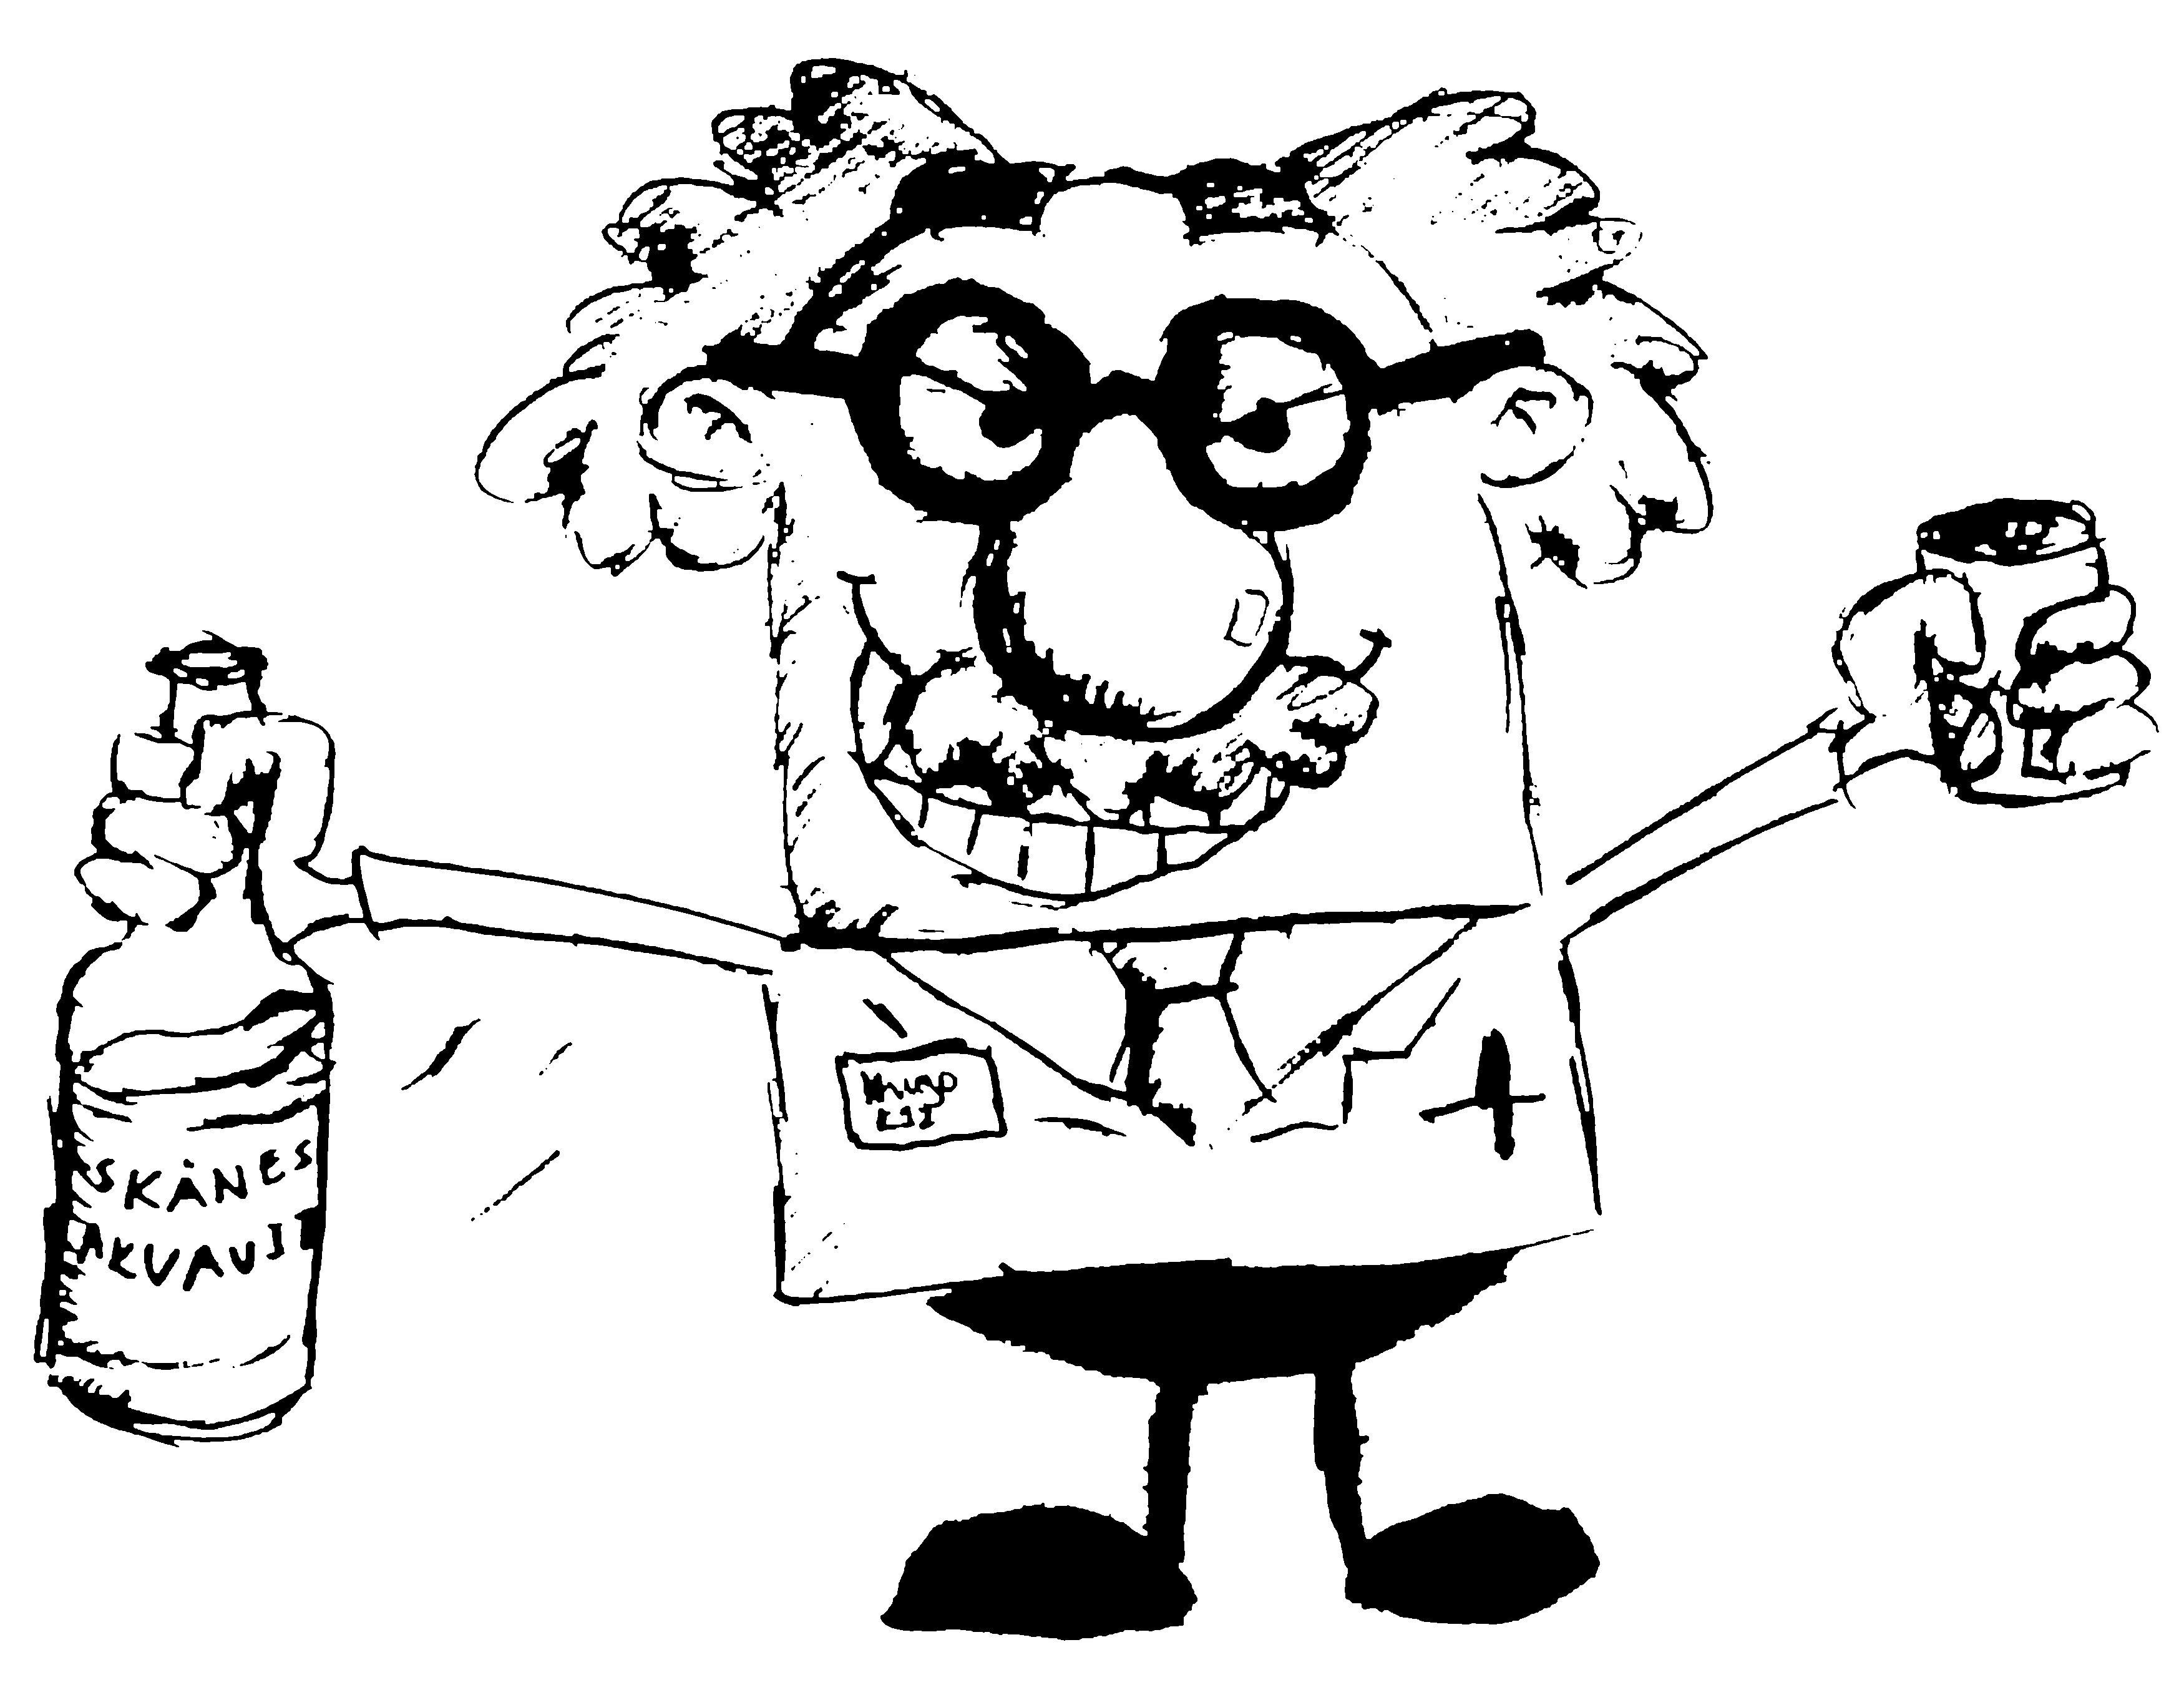
\includegraphics[width=4.5cm]{./bilder/GalenVetenskapsmanTransparent.png}
\end{textblock*}

\subsection*{Det naturliga urvalet} 
\index[alfa]{Det naturliga urvalet}
\index[anfa]{Darwin studerade liv och natur}
\songinfo{Mel: Mors lilla Olle\\
Text: Rolf Malmström}

\begin{parse lines}[\noindent]{#1\\}
    När Darwin studerade liv i natur
    Så fann han att först dör de svagaste djur
    De sämsta bland hjärnceller dör också först
    Så öka din IQ och minska din törst

\end{parse lines}

\subsection*{Lillebror och jag} 
\index[alfa]{Lillebror och jag}
\index[anfa]{Tycker du att snapsen är för stor}
\songinfo{Mel: Måltidssången (refrängen)\\
Lundakarnevalen 1998}

\begin{parse lines}[\noindent]{#1\\}
    Tycker du att snapsen är för stor
    kan du ge en slatt till lillebror
    Både en, både två, både tre, både fem
    och sen blir det fosterhem!

\end{parse lines}


\subsection*{Talteori} 
\index[alfa]{Talteori}
\index[anfa]{1, 2, 75, 6, 7}
\songinfo{Mel: Ritch, ratch}

\begin{parse lines}[\noindent]{#1\\}
    1, 2, 75, 6, 7, 75, 6, 7, 75, 6, 7,
    1, 2, 75, 6, 7, 75, 6, 7, 73,
    107, 103, 102,
    107, 6, 19, 27,
    17, 18, 16, 15,
    13, 19, 14, 17,
    19 16 18 11 
    8 47!
\end{parse lines}
\enlargethispage{1cm}
\newpage

\subsection*{Vikingen} 
\index[alfa]{Vikingen}
\index[anfa]{En viking vill ha livets vann}
\songinfo{Mel: When Johnny comes marching home\\
Text: Olof Ekdahl\\
E-sektionen Sångarstriden 1981}

\begin{parse lines}[\noindent]{#1\\}
    
    En viking vill ha livets vann,
    hurra, hurra!
    Den hastigt i mitt svalg försvann,
    hurra, hurra!
    Till kalv, till oxe, till fisk, till fläsk,
    när kärringen bara dricker läsk,
    då vill alla sanna vikingar ha en bäsk

    När vi druckit bäsken slut,
    tragik, tragik!
    Då bäres varje viking ut,
    som lik sig lik
    Och sen, om vi vaknar, vi sjunger en bit,
    sen korkar vi upp Skånes Akvavit
    ||: Skål för alla vikingar som kom hit!:|| 
\end{parse lines}

\vissteduatt{Visste du att Vikingen skrevs av en E:are? Han heter Olof,\\kallades Öloph, och var sektionens första krögare.}

\newpage

\begin{textblock*}{3cm}(6.1cm,8.5cm) % {width}(x, y)
    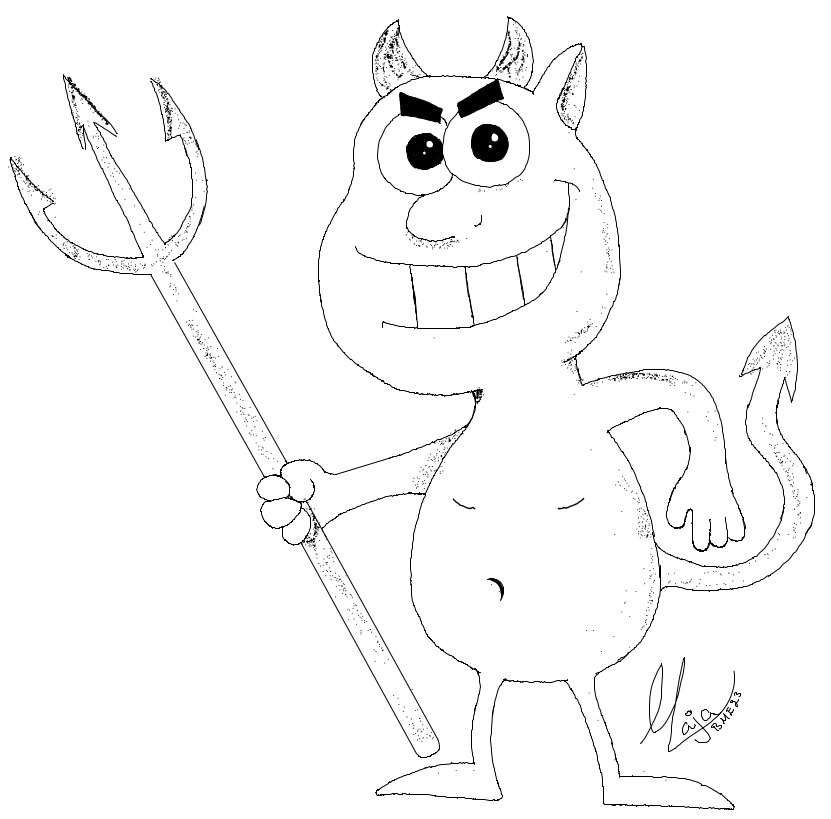
\includegraphics[width=4cm]{./bilder/majas-bilder/devil.png}
\end{textblock*}

\subsection*{Imbelupet} 
\index[alfa]{Imbelupet}
\index[anfa]{Imbelutpet glaset står på bräcklig fot}
\songinfo{Mel: Kors på Idas grav}

\begin{parse lines}[\noindent]{#1\\}
    Imbelupet glaset står på bräcklig fot,
    kalla pilsnerpavor luta sig därmot
    men därnere, miserere,
    uti magens dunkla djup,
    sitter djävulen och väntar på en sup

    uti magens välvda valv, 
    vankar djävulen och ropar på en halv

    uti magen härs och tvärs,
    kilar djävulen och skriker på en ters

    uti magen djup så svart,
    löper djävulen och skränar på en kvart

    uti magens labyrint,
    irrar djävulen och tjoar på en kvint

    uti magens slingerväxt,
    springer djävulen och skriar på en sext

    uti magen heluppknäppt
    rusar djävulen och vrålar på en sept!

    uti magen an och av
    vankar djävulen och väser på oktav
\end{parse lines}

\vissteduatt{Visste du att det finns ett svärd på sektionen? Fråga någon i 
\\KM om Sexmästarsvärdet!}
\newpage

\subsection*{Vi skålar för våra vänner} 
\index[alfa]{Vi skålar för våra vänner}
\index[anfa]{Vi skålar för våra vänner}
\songinfo{Mel: Flickan går i ringen}

\begin{parse lines}[\noindent]{#1\\}
    Vi skålar för våra vänner
    och dom som vi känner
    och dom som vi inte känner
    dom skiter vi i!

    Vi skiter i våra vänner
    och dom som vi känner
    och dom som vi inte känner
    dom skålar vi för!
\end{parse lines}

\subsection*{Den som spar den har} 
\index[alfa]{Den som spar den har}
\index[anfa]{Om man bara tar en smutt, smutt, smutt}
\songinfo{Mel: Nu är glada julen slut}

\begin{parse lines}[\noindent]{#1\\}
    Om man bara tar en 
    smutt, smutt, smutt,
    utav denna lilla 
    hutt, hutt, hutt
    har man ganska mycket kvar,
    men se den som spar han har, 
    inte särskilt roligt
\end{parse lines}

\vissteduatt{Visste du att det finns ett svärd på sektionen? Fråga någon i 
\\E6 om Krögarsvärdet!}

\newpage

\subsection*{Att fela är mänskligt} 
\index[alfa]{Att fela är mänskligt}
\index[anfa]{Trampa på ett smådjur}
\songinfo{Mel: Prästens lilla kråka\\
Lundakarnevalen 2010}

\begin{parse lines}[\noindent]{#1\\}
    Trampa på ett smådjur,
    slakta gulligt rådjur,
    måste göras rätt försiktigt...

    Gifta sig med släkten,
    stjäla ur kollekten,
    det är fel och det är viktigt!

    ||: Men att sjunga en snutt, och ta sig en hutt
    Det är bara rätt och riktigt! :||
\end{parse lines}

\subsection*{Vår höga skatt} 
\index[alfa]{Vår höga skatt}
\index[anfa]{Vår höga skatt, skatt, skatt}
\songinfo{Mel: En kulen natt\\
M-sektionen Sångarstriden 2003}

\begin{parse lines}[\noindent]{#1\\}
    Vår höga skatt, skatt, skatt
    Gör att jag korsar
    En bro till främmande, främmande land
    Där spriten forsar
    Och där jag handlade, handlade sprit
    Som jag sen smugglade, smugglade hit
    Så att en su-petti-petti-petti-pett
    Jag kan få ta
    I detta nu!
\end{parse lines}

\newpage

\subsection*{Häll upp en} 
\index[alfa]{Häll upp en}
\index[anfa]{Häll upp en, häll upp en}
\songinfo{Mel: Pilutta dig\\
E-sektionen Sångarstriden 2000}

\begin{parse lines}[\noindent]{#1\\}
    Häll upp en, häll upp en
    Hell, uppenbart att jag är full
    Du får en, du får en,
    du fåren dom har ull
    Så fort man börjat snapsa har,
    man dricker tills dess inget finnes kvar,
    det kanske, det kanske, det kan skena iväg

    Mitt Valhall, mitt Valhall,
    mitt val - Hallands, det gör så gott
    I magen, I magen, i magen min är flott
    Finess och stil är mitt gebit,
    jag biter aldrig av när jag får sprit,
    jag tar en, jag tar en, jag tar en jäkel till!
\end{parse lines}

\newpage


\subsection*{En gång i månan} 
\index[alfa]{En gång i månan}
\index[anfa]{En gång i månan är månen full}
\songinfo{Mel: Mors lilla Olle}

\begin{parse lines}[\noindent]{#1\\}
    En gång i månan är månen full,
    Men aldrig vi sett honom ramla omkull
    Stum av beundran hur mycket han tål,
    Höja vi glasen och dricka hans skål!

\end{parse lines}


\subsection*{Mjölkade en ko} 
\index[alfa]{Mjölkade en ko}
\index[anfa]{Jag mjölkade en ko idag}
\songinfo{Mel: Jag fångade en räv}

\begin{parse lines}[\noindent]{#1\\}
    Jag mjölkade en ko idag 
    Men när jag såg juvret 
    Då hade jag nog tagit fel 
    För gladast var nog tjuren

\end{parse lines}

\subsection*{Dricka upp} 
\index[alfa]{Dricka upp}
\index[anfa]{Visst kan man dricka långsamt}
\songinfo{Mel: Här kommer Pippi Långstrump}

\begin{parse lines}[\noindent]{#1\\}
    Visst kan man dricka långsamt,
    hälla opp eller ner eller ingen ta
    Visst kan man dricka långsamt,
    men det tänker inte jag!
\end{parse lines}

\newpage
\noBackground

\begin{textblock*}{3cm}(5.5cm,2.8cm) % {width}(x, y)
    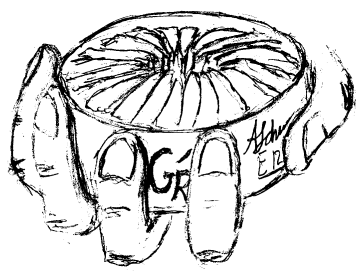
\includegraphics[width=4.5cm]{./bilder/snus.png}
\end{textblock*}


\subsection*{Jag har aldrig varit på snusen} 
\index[alfa]{Jag har aldrig varit på snusen}
\index[anfa]{Jag har aldrig varit på snusen}
\songinfo{Mel: O så saligt att få vandra}

\begin{parse lines}[\noindent]{#1\\}
    Jag har aldrig vatt på snusen,
    aldrig rökat en cigarr - halleluja!
    Mina dygder äro tusen,
    inga syndiga laster jag har

    Jag har aldrig sett nå't naket,
    inte ens ett litet nyfött barn
    Mina blickar går mot taket,
    därmed undgår jag frestarens garn

    ||: Halleluja - halleluja! :||

    Bachus spelar på gitarren,
    Satan spelar på sitt handklaver
    Alla djävlar dansar tango,
    säg vad kan man väl önska sig mer?

    Jo, att alla bäckar vore brännvin,
    stadsparksdammen full av bayerskt öl,
    konjak i varenda rännsten
    och punsch i varendaste pöl

    Och mera öl…
    Vomera öl…
\end{parse lines}

\vissteduatt{Visste du att de första BME-studenterna började på \\
LTH först 2011?}
\newpage
\resetBackground

\subsection*{Jag har aldrig varit på UB} 
\index[alfa]{Jag har aldrig varit på UB}
\index[anfa]{Jag har aldrig varit på UB}
\songinfo{Mel: O så saligt att få vandra\\
E-sektionen Sångarstriden 2009}

\begin{parse lines}[\noindent]{#1\\}
    Jag har aldrig varit på UB,
    aldrig pluggat på Café Athen,
    aldrig skurit upp en snubbe,
    kan ej skilja artär från ven

    Jag har aldrig börjat klockan 9,
    eller slutat 14:32
    I AF-borgen går jag vilse,
    för jag går på LTH

    Dom har aldrig var't på ön Ön,
    aldrig målat Väg och Vattens spik
    Aldrig haft det stora nöjet,
    att få somna till Böijers logik

    Dom har aldrig vunnit en Regatta,
    eller festat i en skitig overall
    Aldrig däckat bakom Lophtet,
    för dom går ej på LTH

    E kan j-omega och Ohms lag
    F och Nano fattar kvantfysik
    Eko, eko, eko, eko,
    eko, eko med akvavit

\end{parse lines}

\newpage

\begin{parse lines}[\noindent]{#1\\}

    I och M kan ragga på kemister
    Data knackar på sin kära linuxkod
    Inga här är humanister,
    för vi är alla LTH

    I och M kan ragga på kemister
    Data knarkar på sin kära linuxkod
    Mardrömmar om humanister,
    drömmer alla på LTH

\end{parse lines}


\subsection*{The BASIC song} 
\index[alfa]{The BASIC song}
\index[anfa]{LET oss nu fatta}
\songinfo{Mel: Mors lilla Olle}

\begin{parse lines}[\noindent]{#1\\}
    \textcolor{gray}{\texttt{10}} \texttt{LET} oss nu fatta i våra glas 
    \textcolor{gray}{\texttt{20}} \texttt{INPUT} en klunk utav det som där has 
    \textcolor{gray}{\texttt{30}} \texttt{IF} du fått nog \texttt{THEN} till \texttt{50} min vän 
    \textcolor{gray}{\texttt{40}} \texttt{ELSE GOTO}-baka till \texttt{10} igen 
    \textcolor{gray}{\texttt{50}} \texttt{END}

\end{parse lines}


\vissteduatt{Visste du att innan pandemin skrevs alla programmeringstentor\\
 med papper och penna?}
\newpage



\begin{textblock*}{3cm}(5.2cm,7.5 cm) % {width}(x, y)
    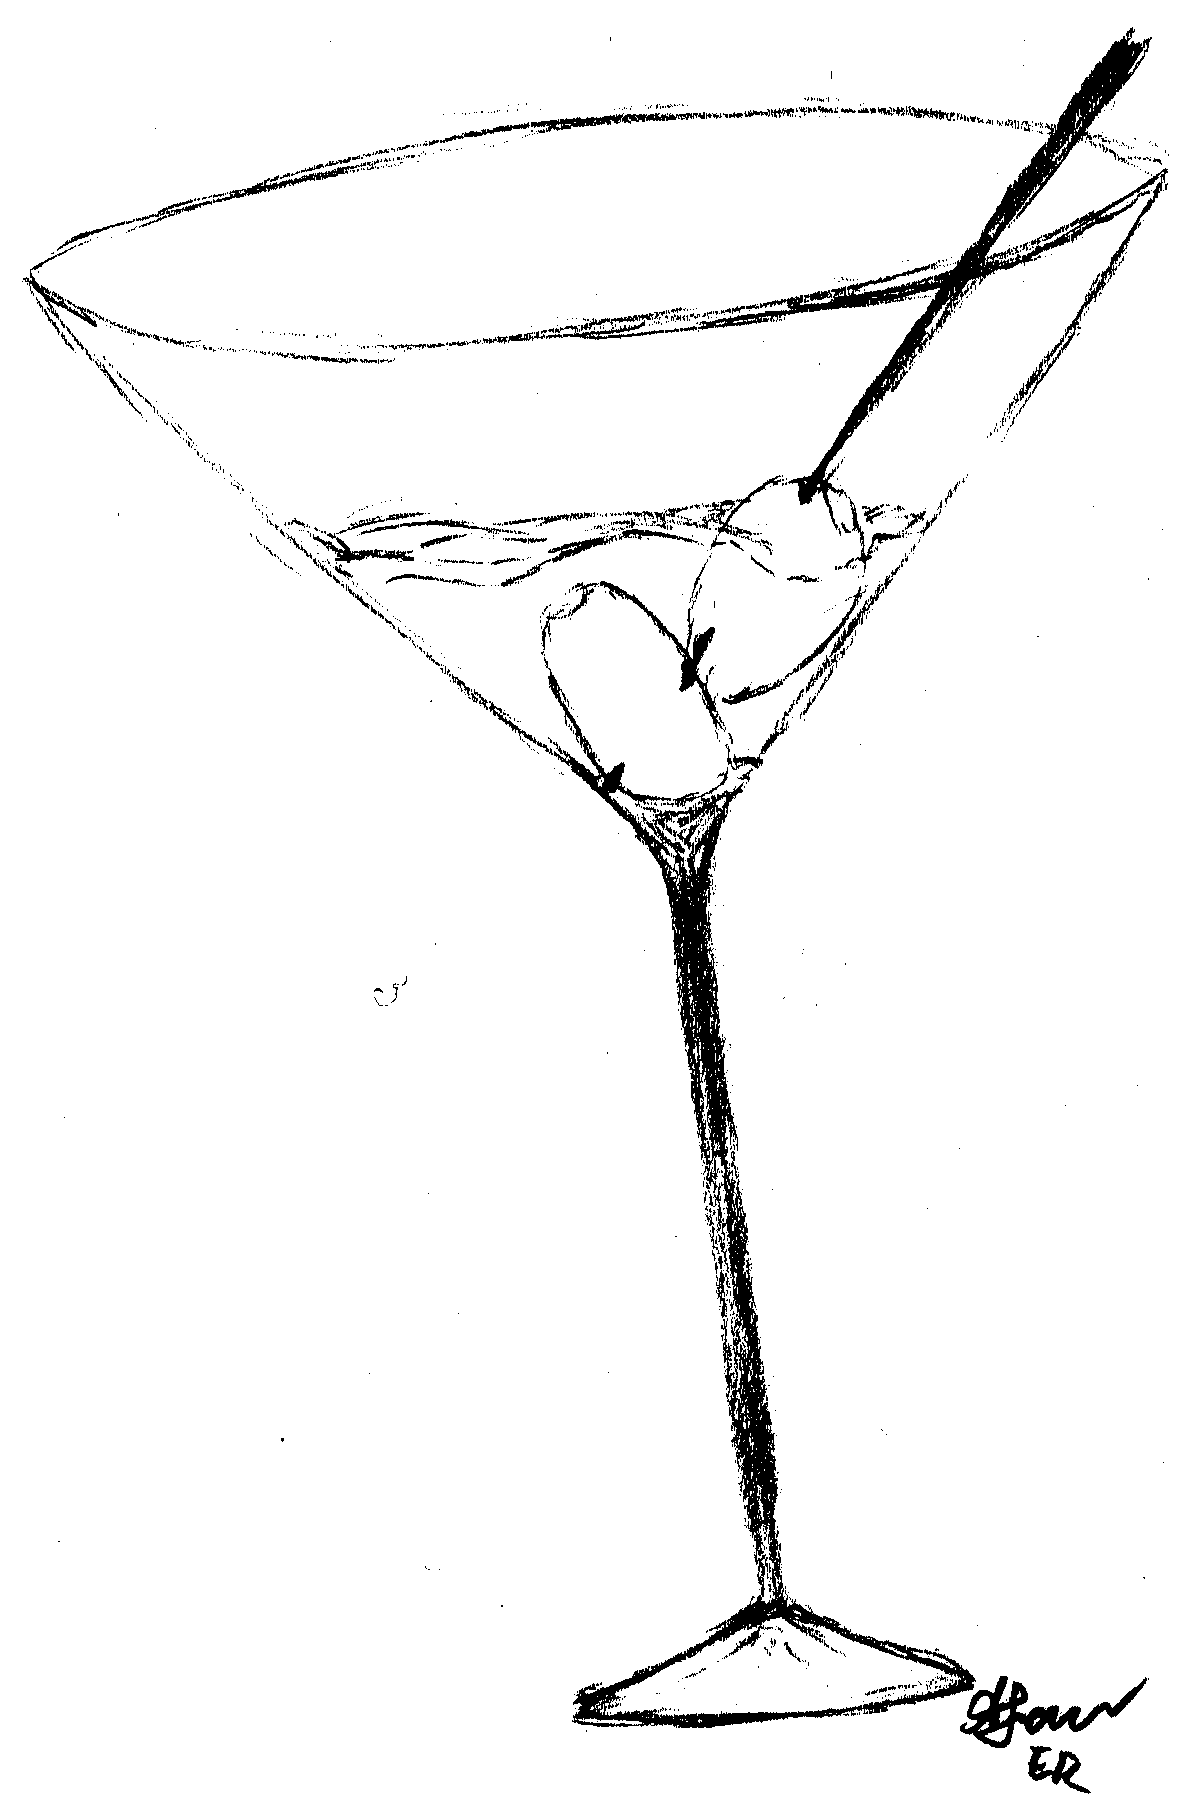
\includegraphics[width=4.0cm]{./bilder/ub.png}
\end{textblock*}




\subsection*{De som är nyktra} 
\index[alfa]{De som är nyktra}
\index[anfa]{De som är nyktra}
\songinfo{Mel: Du är den ende}

\begin{parse lines}[\noindent]{#1\\}
    De som är nyktra 
    har inte så roligt,
    de har bara ansvar 
    och inte nåt 
    tjolittanlej faderulla 
    men vi som är fulla 
    vi har bara kul nästan jämt

    Det sägs att en män'ska 
    kan va' utan brännvin,
    det stämmer måhända 
    men se blott på den min
    som pryder en absolutist, 
    den e' jävligt trist
    därför så sjunger vi nu:

    De som är nyktra 
    har inte så roligt,
    de har bara ansvar 
    och inte nåt 
    tjolittanlej faderulla 
    men vi som är fulla 
    vi har bara kul nästan jämt
\end{parse lines}

\vissteduatt{Visste du att 1996 började 272 teknologer på E? De var indelade i\\8 klasser med ungefär 32 i varje.}
\newpage


\subsection*{Vi som är nyktra} 
\index[alfa]{Vi som är nyktra}
\index[anfa]{Vi som är nyktra}
\songinfo{Mel: Du är den ende}

\begin{parse lines}[\noindent]{#1\\}
    Vi som är nyktra
    vi har faktiskt roligt.
    Jo visst har vi ansvar,
    men minst lika
    tjolittanlej faderulla
    som ni som är fulla
    som tror ni har kul nästan jämt

    Men tänk då efter
    uppå dagen efter
    de dagar med fester,
    med smärtsamma rester
    utav eran hjärna,
    nog tycker ni gärna.
    Att va nykterist är nåt visst

    Vi som är nyktra,
    vi har bara roligt
    Imorrn kan vi
    återigen ha det
    tjolittanlej faderulla,
    men ni som är fulla
    aj, aj, aj, det är väl för trist
\end{parse lines}



\newpage

\subsection*{Mera brännvin} 
\index[alfa]{Mera brännvin}
\index[anfa]{Mera brännvin i glasen}
\songinfo{Mel: Internationalen}

\begin{parse lines}[\noindent]{#1\\}
    Mera brännvin i glasen,
    mera glas på vårt bord,
    mera bord på kalasen,
    mer kalas på vår jord

    Mera jordar med måne,
    mera månar i mars,
    mera marscher till Skåne,
    mera Skåne, Gud bevars, bevars, bevars!
\end{parse lines}

\subsection*{En kulen snaps} 
\index[alfa]{En kulen snaps}
\index[anfa]{En kulen snaps}
\songinfo{Mel: En kulen natt}

\begin{parse lines}[\noindent]{#1\\}
    En kulen snaps, snaps, snaps
    Den står vid faten
    Om jag nu vågade, vågade
    ta den före maten
    Men värden håller ett jäkla långt tal
    Kanske min snaps inte längre hålls sval
    Så ner i djupetetetet
    Den snapsen slank
    Menns den var kall!
\end{parse lines}

\vissteduatt{Visste du att det finns en finsk version av Mera Brännvin?\\Se Internationella visor!}

\newpage


\subsection*{Feministvikingen} 
\index[alfa]{Feministvikingen}
\index[anfa]{En viking viker tvätten själv}
\songinfo{Mel: When Johnny Comes Marching Home}

\begin{parse lines}[\noindent]{#1\\}
    En viking viker tvätten själv
    Hurra hurra!
    Ordet "viking" kommer sig därav, jaha!
    Föräldraledigheten delas exakt
    När vikingen sina barn har lagt
    Då är vikingens fru ute på jakt

    En viking vill ha livets vann
    Hurra hurra!
    Men på sig själv han lägger band,
    Jaha, vad bra!
    Mjödet prioriteras sist,
    Tvätta och städa blir aldrig trist
    För våran viking, han är feminist
\end{parse lines}

\subsection*{Änglahund} 
\index[alfa]{Änglahund}
\index[anfa]{Det står en hund}
\songinfo{Mel: Marseljäsen
\\ V-sektionen sångarstriden 1991}

\begin{parse lines}[\noindent]{#1\\}
    Det står en hund på fjärde våningen 
    och den tänker hoppa ner!
    BANZAI!
    Det var en japanesisk självmordhund 
    och den hoppar aldrig mer!
\end{parse lines}



\newpage

\subsection*{Nu dags taga sig en snaps strax} 
\index[alfa]{Nu dags taga sig en snaps strax}
\index[anfa]{Nu dags taga sig en snaps strax}
\songinfo{Mel: Can-Can}

\begin{parse lines}[\noindent]{#1\\}
    Nu dags
    taga sig en snaps strax,
    som din kropp tar opp och
    låter rinna ner
    Och ger dig smak för flera

    Ditt liv,
    blott ett tidsfördriv, du 
    kastar ner en kask och 
    lever glatt och ler,
    när fler du ser

    Med sill,
    eller vad du vill till,
    håll din strupe våt, åt
    Bacchus ge din själ,
    han vill dig bara väl

    Så skjut 
    först en kort salut ut
    nu tar sången slut, trut
    Gapa, svälj och njut!
\end{parse lines}

\vissteduatt{Visste du att E-sektionen var först på LTH att införa ett\\permanent alkoholtillstånd?}
\newpage
\noBackground

\begin{textblock*}{3cm}(6.7cm,1.0cm) % {width}(x, y)
    
\includegraphics[width=1.4cm]{./bilder/humla.png}
\end{textblock*}
\begin{textblock*}{3cm}(7.2cm,2.2cm) % {width}(x, y)
    
\includegraphics[width=3cm]{./bilder/humla_signerad.png}
\end{textblock*}
\begin{textblock*}{3cm}(6.9cm,4.9cm) % {width}(x, y)
    
\includegraphics[width=1.6cm]{./bilder/humla.png}
\end{textblock*}
\begin{textblock*}{3cm}(8.0cm,5.9cm) % {width}(x, y)
    
\includegraphics[width=2cm]{./bilder/humla.png}
\end{textblock*}
\begin{textblock*}{3cm}(6.0cm,9.0cm) % {width}(x, y)
    
\includegraphics[width=1.4cm]{./bilder/humla.png}
\end{textblock*}

\subsection*{Humlorna} 
\index[alfa]{Humlorna}
\index[anfa]{Vi äro små humlor vi bzz, bzz}
\songinfo{Mel: Här kommer Karl-Alfred boy}

\begin{parse lines}[\noindent]{#1\\}
    ||: Vi äro små humlor vi bzz, bzz :||
    Vi äro små humlor som tar oss en geting
    Vi äro små humlor vi bzz, bzz

    ||: Vi äro små fiskar vi blubb, blubb :||
    Vi äro små fiskar som tar oss en kallsup
    Vi äro små fiskar vi blubb, blubb

    ||: Vi äro små änglar vi flax, flax :||
    Vi äro små änglar som tar oss en Djävel
    Vi äro små änglar vi flax, flax
\end{parse lines}

\subsection*{Stopp en stund} 
\index[alfa]{Stopp en stund}
\index[anfa]{Stopp en stund med skratt och pratet}
\songinfo{Mel: Räven raskar över isen}

\begin{parse lines}[\noindent]{#1\\}
    Stopp en stund med skratt och pratet,
    kniv och gaffel lägg på fatet
    Seden är, att så här,
    man handskas med destilatet

    Man lyfter glaset med höger hand,
    och trycker läpparna mot dess rand
    Man dricker ur, och grinar sur,
    och väntar på resultatet
\end{parse lines}

\newpage
\resetBackground

% \begin{center}
    \vspace*{1.5cm}
    {\fontsize{20}{20}\textbf{Rekursiva visor}}\\
    \vspace{0.7cm}
    {\fontsize{12}{12}\textit{Om tålamodet själv får välja}}
\end{center}
\addtocwithheader{Rekursiva visor}  % Add entry to TOC and set header\noBackground
\noBackground

\newpage
\resetBackground

\subsection*{Min gode vän Joel} 
\index[alfa]{Min gode vän Joel}
\index[anfa]{Min gode vän Joel}
\songinfo{Mel: Trampa på gasen}

\begin{parse lines}[\noindent]{#1\\}
    Min gode vän Joel
    Han är en glad kamrat
    Han har äpplen fram och en kulvert bak
    Min gode vän Joel
    Han ser rätt lustig ut
    Man kan kalla honom Knut
    Om man vill
    Och det vill man
\end{parse lines}

\subsection*{Vår gode vän Jor-el} 
\index[alfa]{Vår gode vän Jor-el}
\index[anfa]{Vår gode vän Jor-el}
\songinfo{Lundakarnevalen 2002}

\begin{parse lines}[\noindent]{#1\\}
    Vår gode vän Jor-El
    Är far till Superman
    Super man som han blir man full som fan
    Min gode vän Jor-El
    Han dricker supersprit
    Men tål inte kryptonit
    Kastar upp i raketen
\end{parse lines}


\newpage

\subsection*{Min Gode Vän Josef} 
\index[alfa]{Min Gode Vän Josef}
\index[anfa]{Min Gode Vän Josef}
\songinfo{Lundakarnevalen 2006}

\begin{parse lines}[\noindent]{#1\\}
    Min gode vän Josef
    Han var på fyllefest
    I tequilarace - han drack allra mest
    Den helige ande
    Slog till och passa på
    Maria kunde inte gå
    På nio månader
\end{parse lines}

\subsection*{Bortom IT-Samhället} 
\index[alfa]{Bortom IT-Samhället}
\index[anfa]{Usama Bin-Ladin}
\songinfo{Lundakarnevalen 2002}

\begin{parse lines}[\noindent]{#1\\}
    Usama Bin-Ladin
    Har ingen SMS
    Ingen ICQ eller mailadress
    Usama Bin-Ladin
    Tycks ha gått upp i rök
    Man kan inte trycka "Sök"
    Om man vill
    Och det vill Bush
\end{parse lines}

\vissteduatt{Visste du att E-sektionen var den sista sektionen på LTH att skapa\\ en egen sångbok?}

\newpage

\subsection*{Jag pluggar på LU} 
\index[alfa]{Jag pluggar på LU}
\index[anfa]{Jag pluggar på LU}
%\songinfo{}
\begin{parse lines}[\noindent]{#1\\}

    Jag pluggar på LU
    Och läser gratispoäng
    När ni gör er labb
    Ligger jag i säng
    Jag pluggar på LU
    Tar inga hårda tag
    Men ändå får jag bidrag
    Från CSN
    Ja, det får jag   

\end{parse lines}

\subsection*{Jag kuggade tentan} 
\index[alfa]{Jag kuggade tentan}
\index[anfa]{Jag kuggade tentan}
%\songinfo{}

\begin{parse lines}[\noindent]{#1\\}

    Jag kuggade tentan
    Men det gör inte nått
    För jag hade ändå inga pengar fått
    För om man blir ratad
    Av hela CSN
    Får man ofta ringa hem
    För att få lite pengar    
\end{parse lines}


\newpage

\begin{textblock*}{3cm}(4.4cm,8.3cm) % {width}(x, y)
    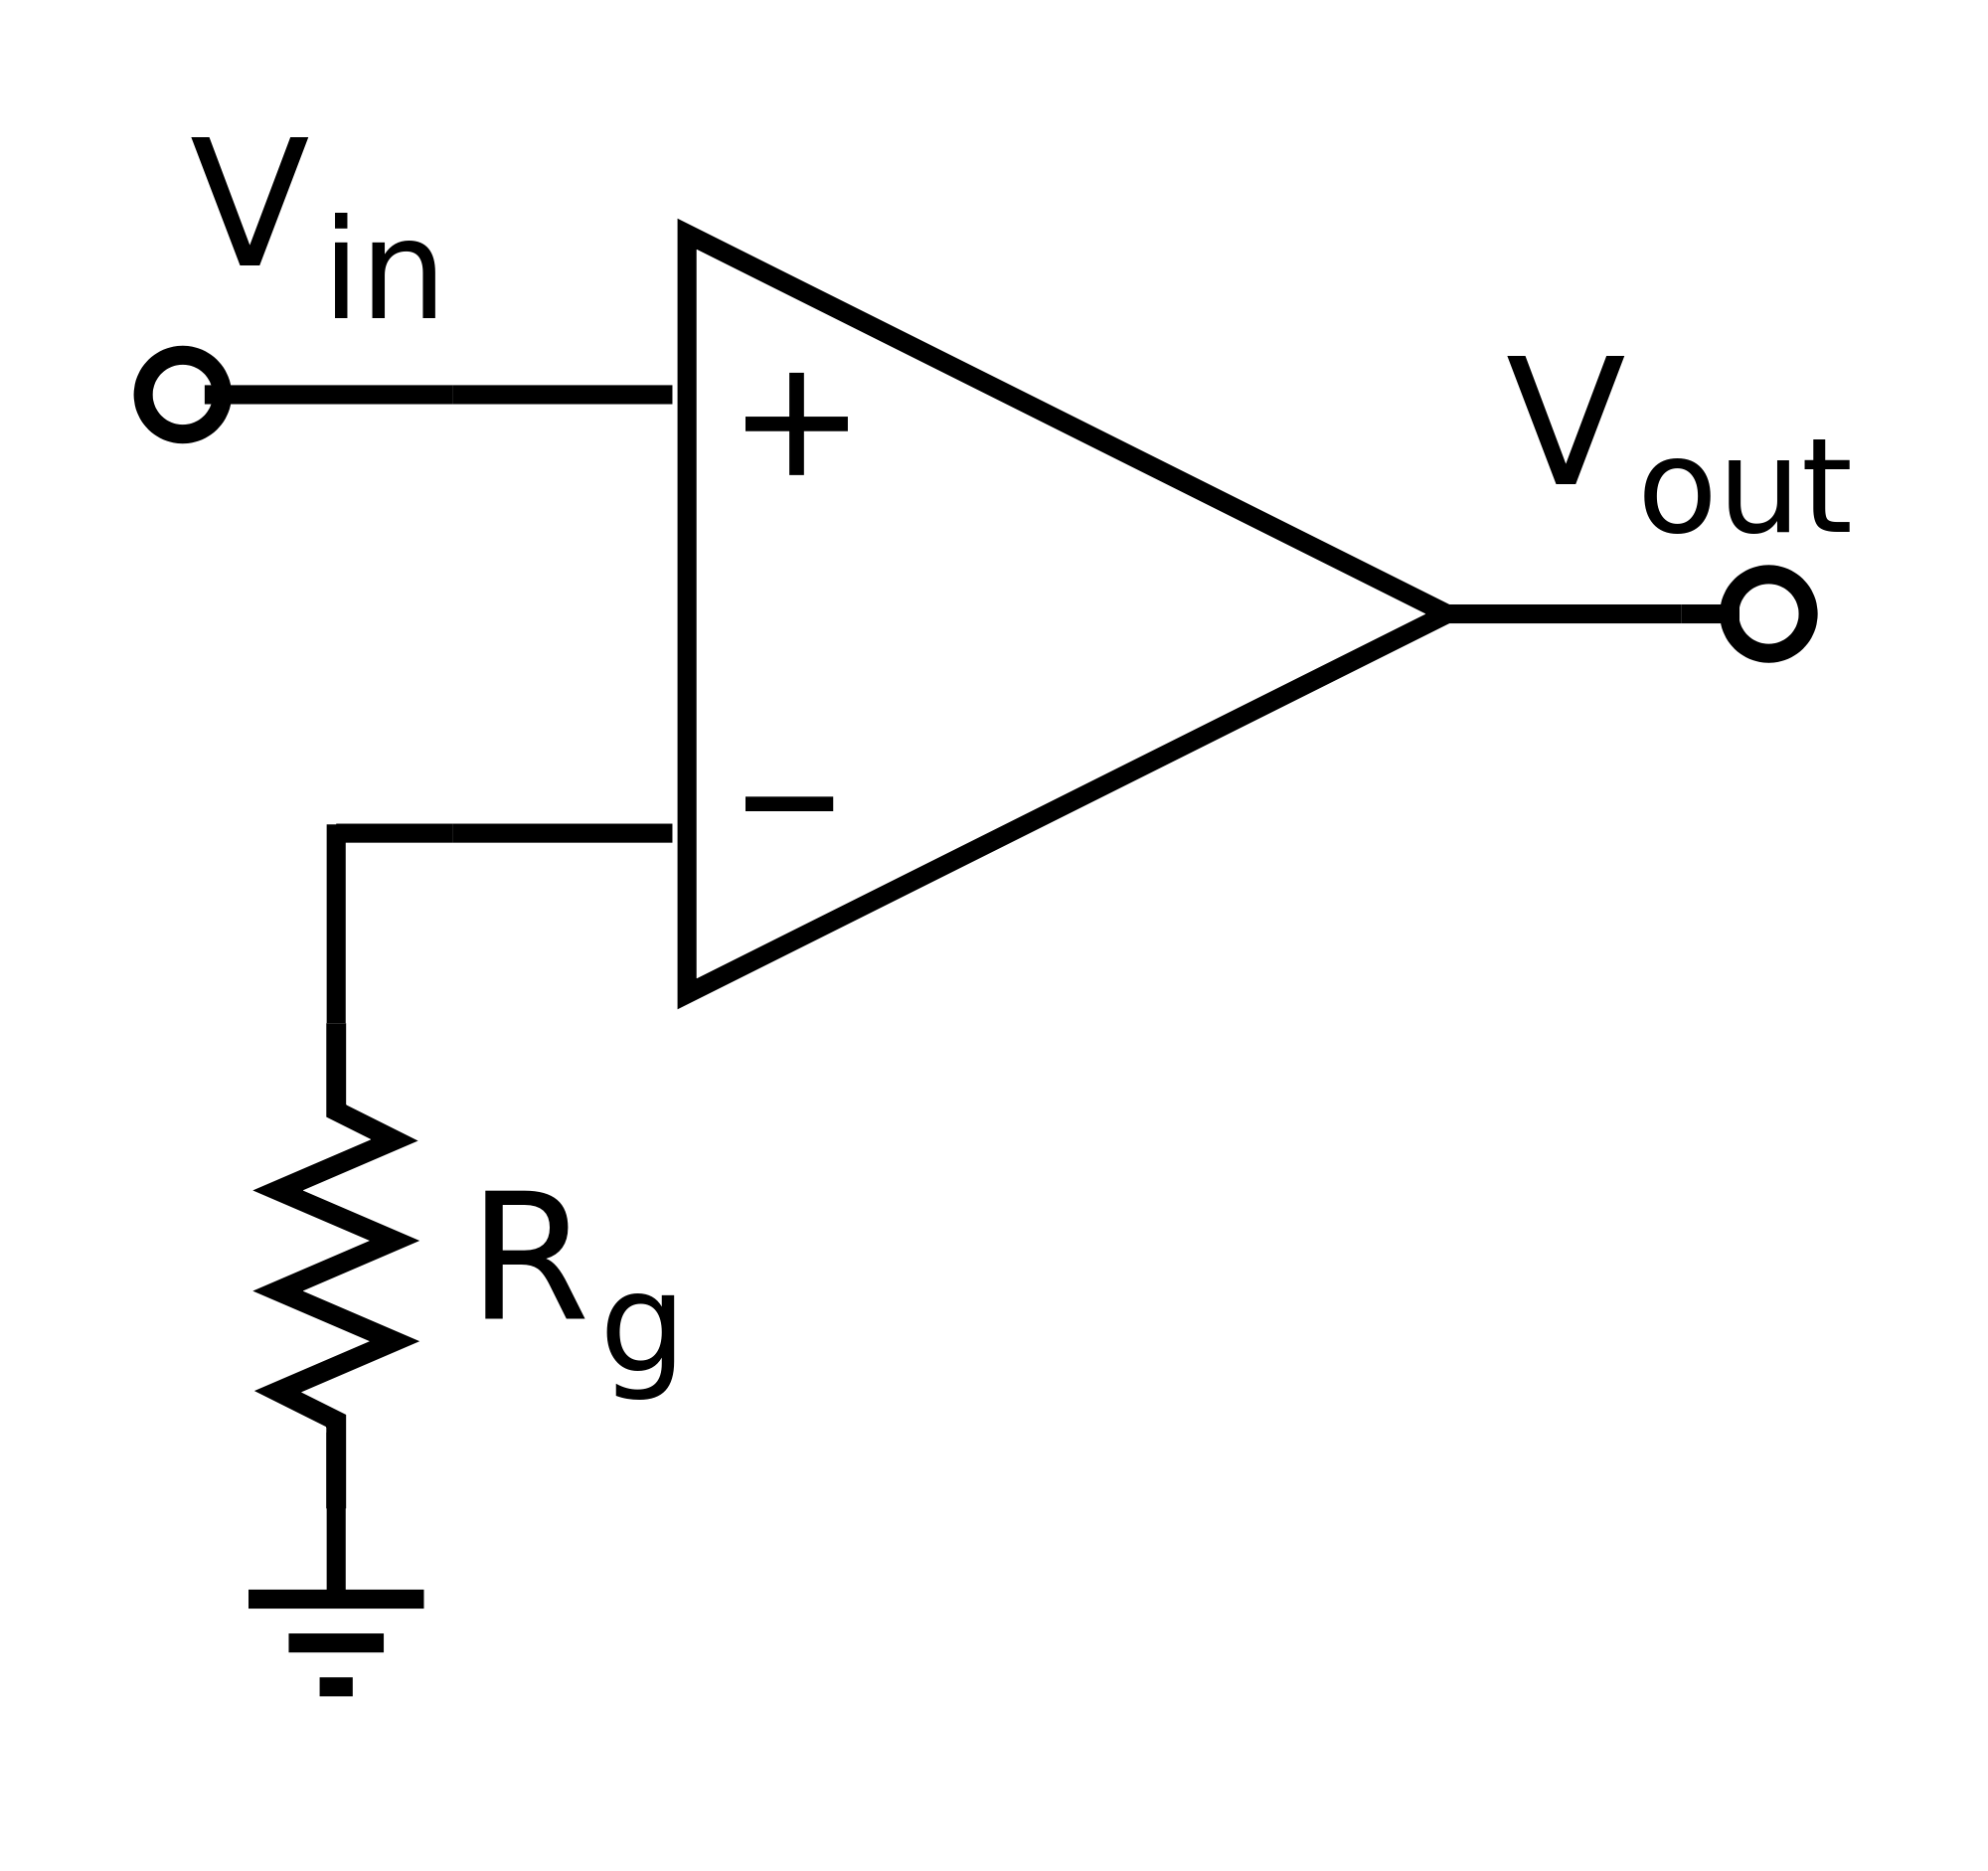
\includegraphics[width=5.6cm]{./bilder/OP-förstärkare.png}
\end{textblock*}


\subsection*{Jag drikker Tuborg} 
\index[alfa]{Jag drikker Tuborg}
\index[anfa]{Jag drikker Tuborg}
\songinfo{Mel: Trampa på gasen\\
synge på dansk}

\begin{parse lines}[\noindent]{#1\\}
    Jeg drikker Tuborg
    og snapser gammeldansk
    Det ær alt jeg vil,
    det ær alt jeg kan
    Jeg drikker Tuborg
    og snapser gammeldansk
    Det ær alt jeg vil og kan,
    så hold kæft jeg ær lykkelig!
\end{parse lines}

\subsection*{Alla är söta} 
\index[alfa]{Alla är söta}
\index[anfa]{Alla på eko}
%\songinfo{}

\begin{parse lines}[\noindent]{#1\\}

    Alla på eko
    Har koll på vårt klimat
    Utan dom får vi förgiftad mat
    Och dom på Eko
    Älskar alla djur
    Och det tycker vi är tur
    För dom är så söta   
\end{parse lines}

\newpage

\subsection*{Måsen} 
\index[alfa]{Måsen}
\index[anfa]{Det satt en mås på en klyvarbom}
\songinfo{Mel: När månen vandrar}

\begin{parse lines}[\noindent]{#1\\}
    Det satt en mås på en klyvarbom
    Och tom i krävan var kräket
    Och tungan lådde i skeppar'ns gom
    Där han satt uti bleket
    Jag vill ha sill hördes måsen rope
    Och skeppar'n svarte: Jag vill ha OP
    Om blott jag får, om blott jag får
    
    Nu lyfter måsen från klyvarbom
    Och vinden spelar i tågen
    OP:n svalkat har skeppar'ns gom
    Jag önskar blott att jag såg 'en
    Så nöjd och lycklig, den arme saten
    Han sätter storsegel den krabaten
    Till sjöss han far, och halvan tar
    
    Den mås som satt på en klyvarbom
    Den är nu död och begraven
    Och skeppar'n som drack en flaska rom
    Han har nu drunknat i haven
    Så kan det gå om man fått för mycké
    Om man för brännvin har fattat tycke
    Vi som har kvar, vi resten tar
    
\end{parse lines}

\newpage

\subsection*{Musen} 
\index[alfa]{Musen}
\index[anfa]{Det satt en mus i en hushållsost}
%\songinfo{}

\begin{parse lines}[\noindent]{#1\\}
    Det satt en mus i en hushållsost
    Och åt och åt utan måtta
    Tills osten blivit en mushåls-ost
    Och han en klotformad råtta
    "Så bra", sa musen, "att va en fettboll,
    Nu kan jag rulla med hast åt rätt håll:
    Ostindien! Ostindien!"
\end{parse lines}

\subsection*{Moosen} 
\index[alfa]{Moosen}
\index[anfa]{Det satt en älg i en klyvartopp}
%\songinfo{}
\begin{parse lines}[\noindent]{#1\\}
    Det satt en älg i en klyvartopp
    Förklädd i älgjaktens månad
    Han var befjädrad till horn och kropp
    Och skepparn blev smått förvånad
    "Jag är en mås, goa skepparn" ljög den
    Förklädda älgen, därefter flög den
    Mjukt föll han sen
    På skepparen
\end{parse lines}

\subsection*{Mesen} 
\index[alfa]{Mesen}
\index[anfa]{Det satt en mes i en klyvarmast}
%\songinfo{}

\begin{parse lines}[\noindent]{#1\\}
    Det satt en mes i en klyvarmast
    Där sågs han ragla och svaja
    För trots att frön var hans enda last
    Var han full som en kaja
    "Vad har du gjort!" hördes skepparn stöna
    Och mesen svarte "Jag rökte fröna
    I egen holk, i egen holk"
\end{parse lines}

\newpage

\subsection*{Boten} 
\index[alfa]{Boten}
\index[anfa]{Min kompis Anna, hon är en bot}
%\songinfo{}

\begin{parse lines}[\noindent]{#1\\}
    Min kompis Anna, hon är en bot
    Hon rensar upp i kanalen
    Och varje gång jag hör hennes låt
    Så får jag ont i analen
    Jag är så trött på den jävla låten
    Kan någon vänlig själ banna boten?
    Jag vete fan
    Jag fick en ban
\end{parse lines}

\subsection*{Kompistipset} 
\index[alfa]{Kompistipset}
\index[anfa]{Min kompis Bosse, en bigamist}
%\songinfo{}

\begin{parse lines}[\noindent]{#1\\}
    Min kompis Bosse, en bigamist
    Tar alltid två öl i baren
    Han säger "Allting kan verka trist
    Ifall man blott bara tar en
    Nej, ta och skaffa dig en till fru å
    Be alltid bartendern om en duo
    Så skål min vän, och skål igen!"
\end{parse lines}

\subsection*{När månen vandrar} 
\index[alfa]{När månen vandrar}
\index[anfa]{När månen vandrar sin tysta ban}
%\songinfo{}

\begin{parse lines}[\noindent]{#1\\}
    När månen vandrar sin tysta ban
    Och tittar in genom rutan
    Då tänker jag, att på ljusan da'n
    Då kan jag klara mig utan
    Då kan jag klara mig utan måne
    Men utan Renat och utan Skåne?
    Det vete fan, det vete fan    
\end{parse lines}

\newpage

\subsection*{När måsen vandrar} 
\index[alfa]{När måsen vandrar}
\index[anfa]{Om du en sittning vill sakta ner}
%\songinfo{}

\begin{parse lines}[\noindent]{#1\\}
    Om du en sittning vill sakta ner 
    och alla gästerna störa 
    Ja då räcker det att de ser 
    att de nu måsen ska köra 
    Den jävla låten, den är så tråkig 
    “Men den här texten är inte pjåkig” 
    Den åker ut 
    Så håll din trut
\end{parse lines}

\subsection*{JAS:en} 
\index[alfa]{JAS:en}
\index[anfa]{Där flög en JAS över Västerbron}
%\songinfo{}

\begin{parse lines}[\noindent]{#1\\}
    Där flög en JAS över Västerbron
    Men styrsystemet var trasigt
    Piloten sköt ut sig med kanon
    För planet svängde så knasigt
    "Jag vill ju uppåt, jag vill ju mer"
    Men planet svarte: "Jag vill ju ner
    Mot alla hjon, på Västerbron" 
\end{parse lines}


\begin{textblock*}{10cm}(0.0cm, 0.5cm) % {width}(x, y)
    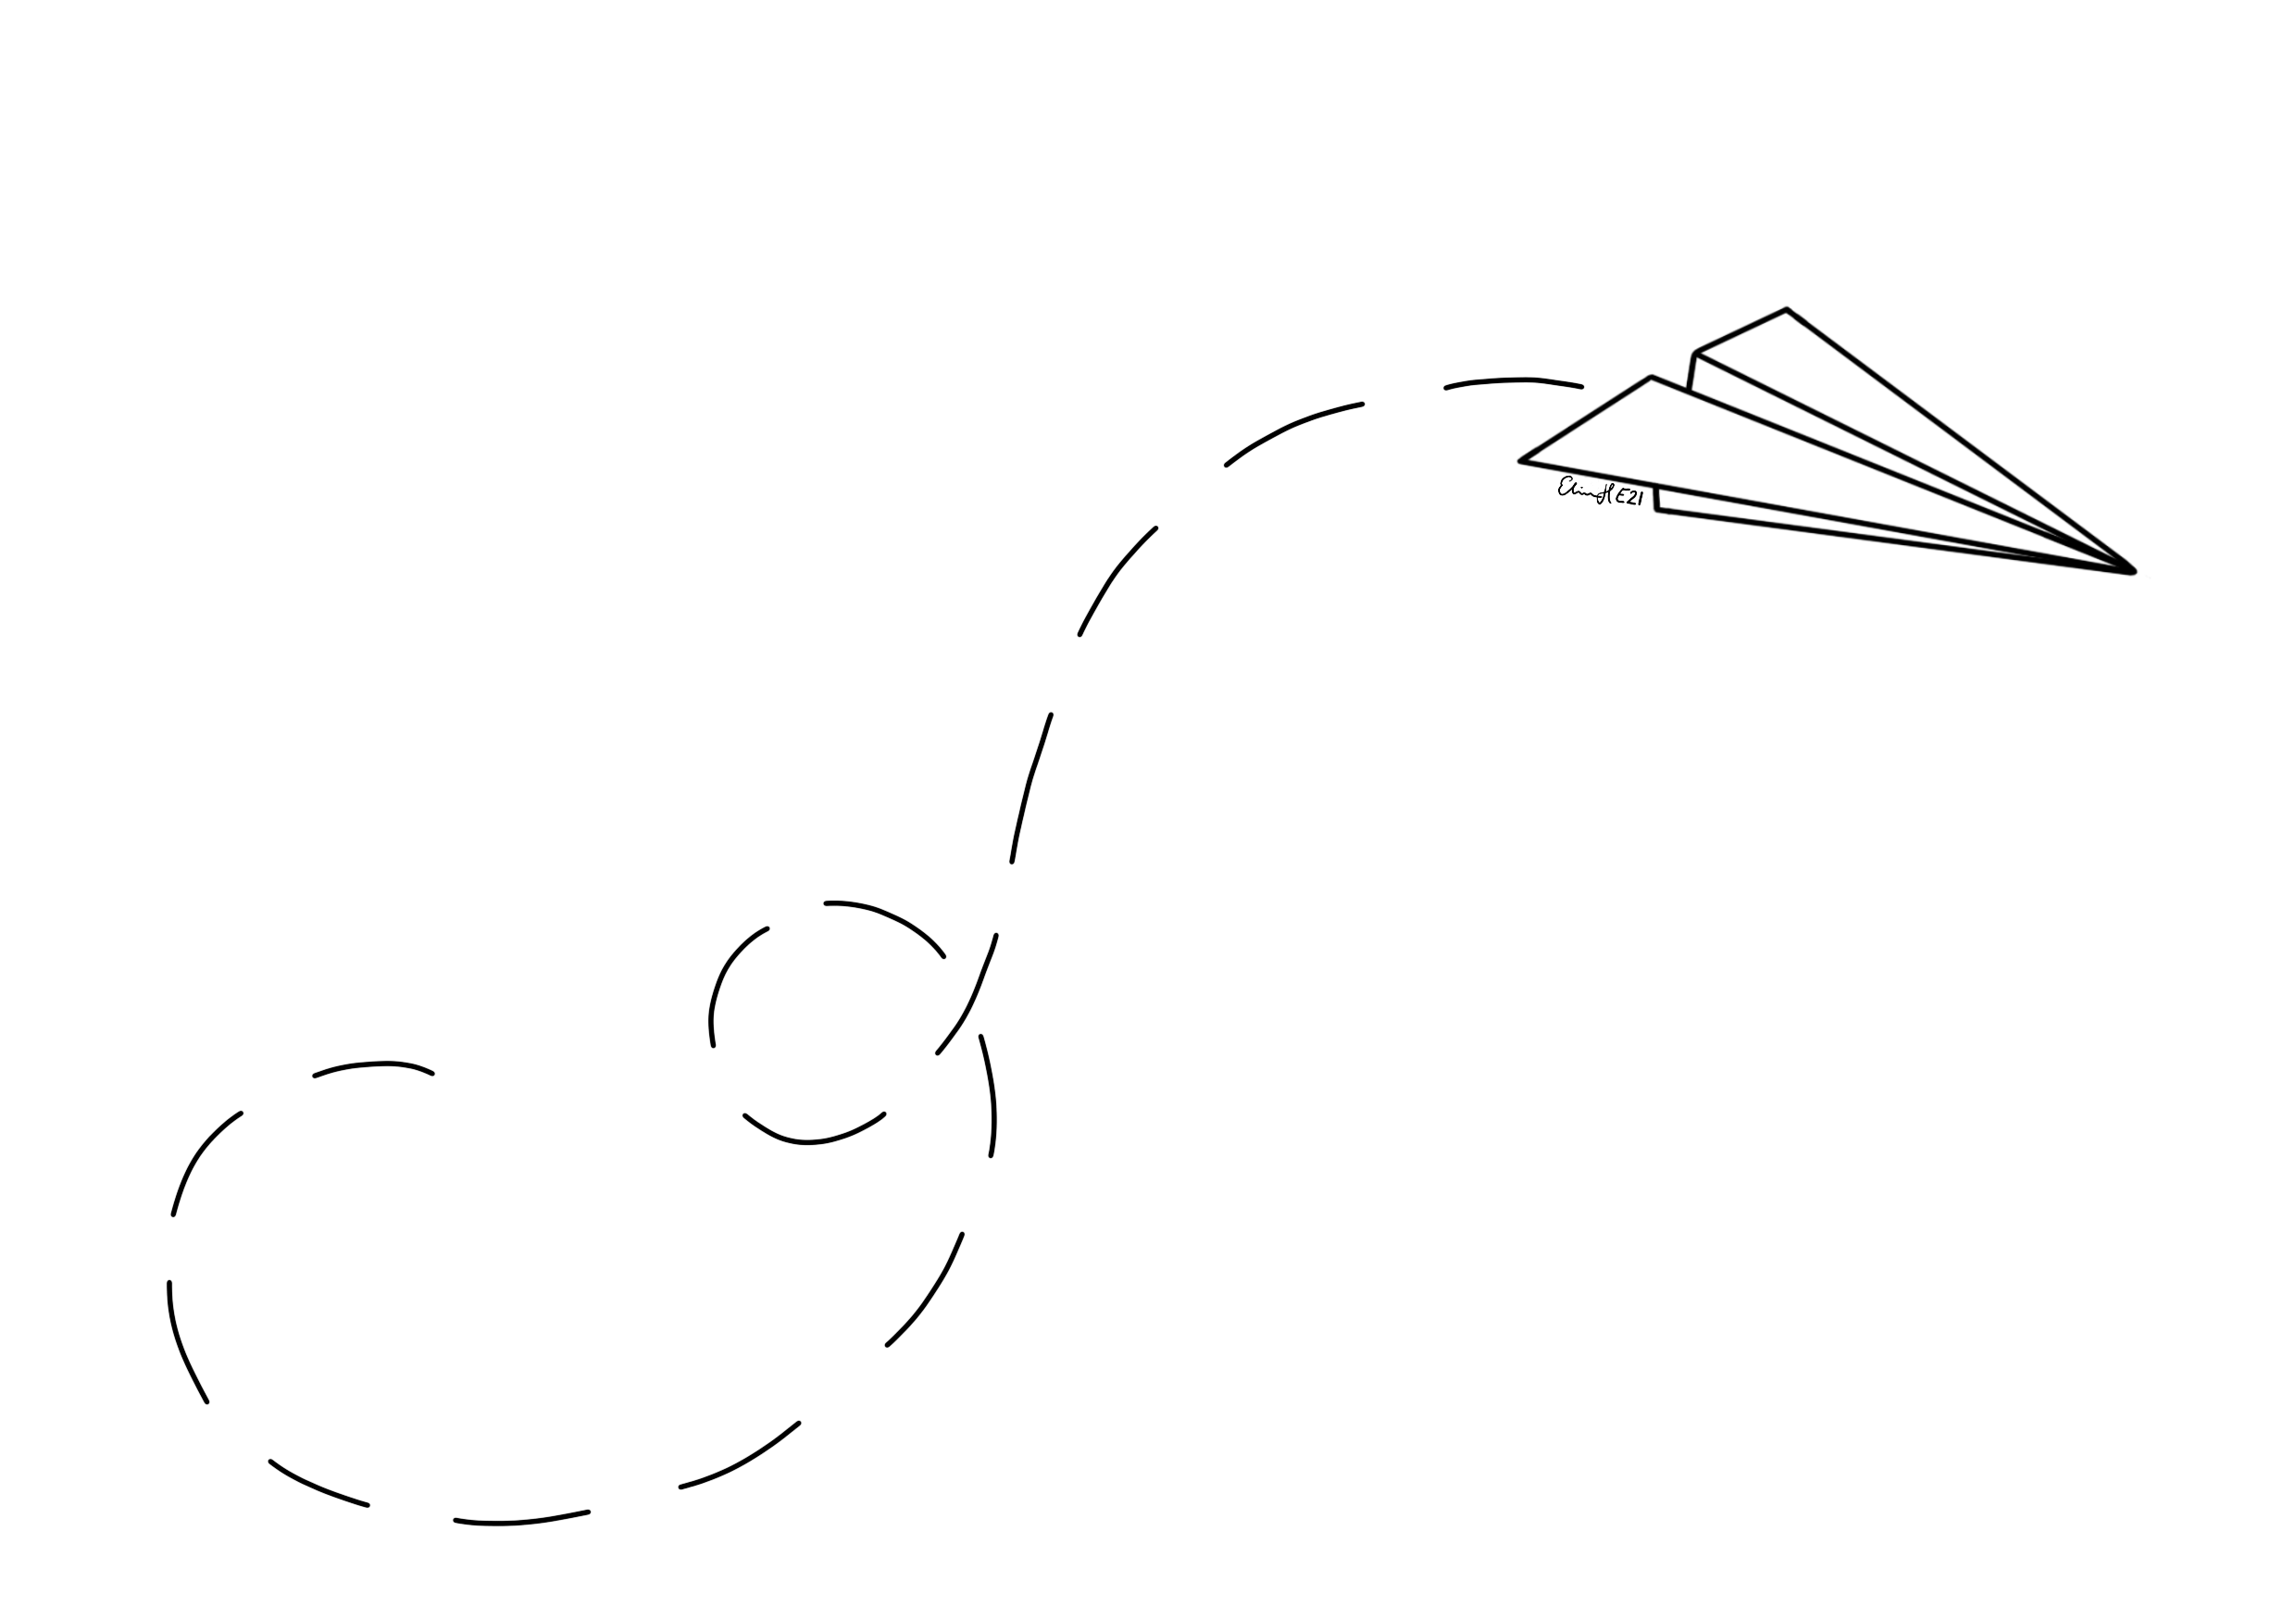
\includegraphics[width=20cm]{./bilder/pappersplan_signerad.png}
\end{textblock*}

\newpage
\noBackground

\begin{comment}
\begin{textblock*}{10cm}(1.0cm, 1.0cm) % {width}(x, y)
    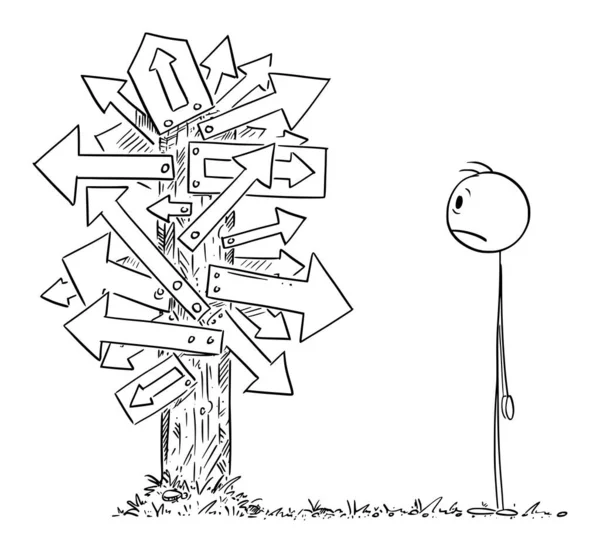
\includegraphics[width=20cm]{./bilder/roda_havet_test.png}
\end{textblock*}

\vspace*{5cm}
\end{comment}

\begin{textblock*}{10cm}(-10.3cm, 0.3cm) % {width}(x, y)
    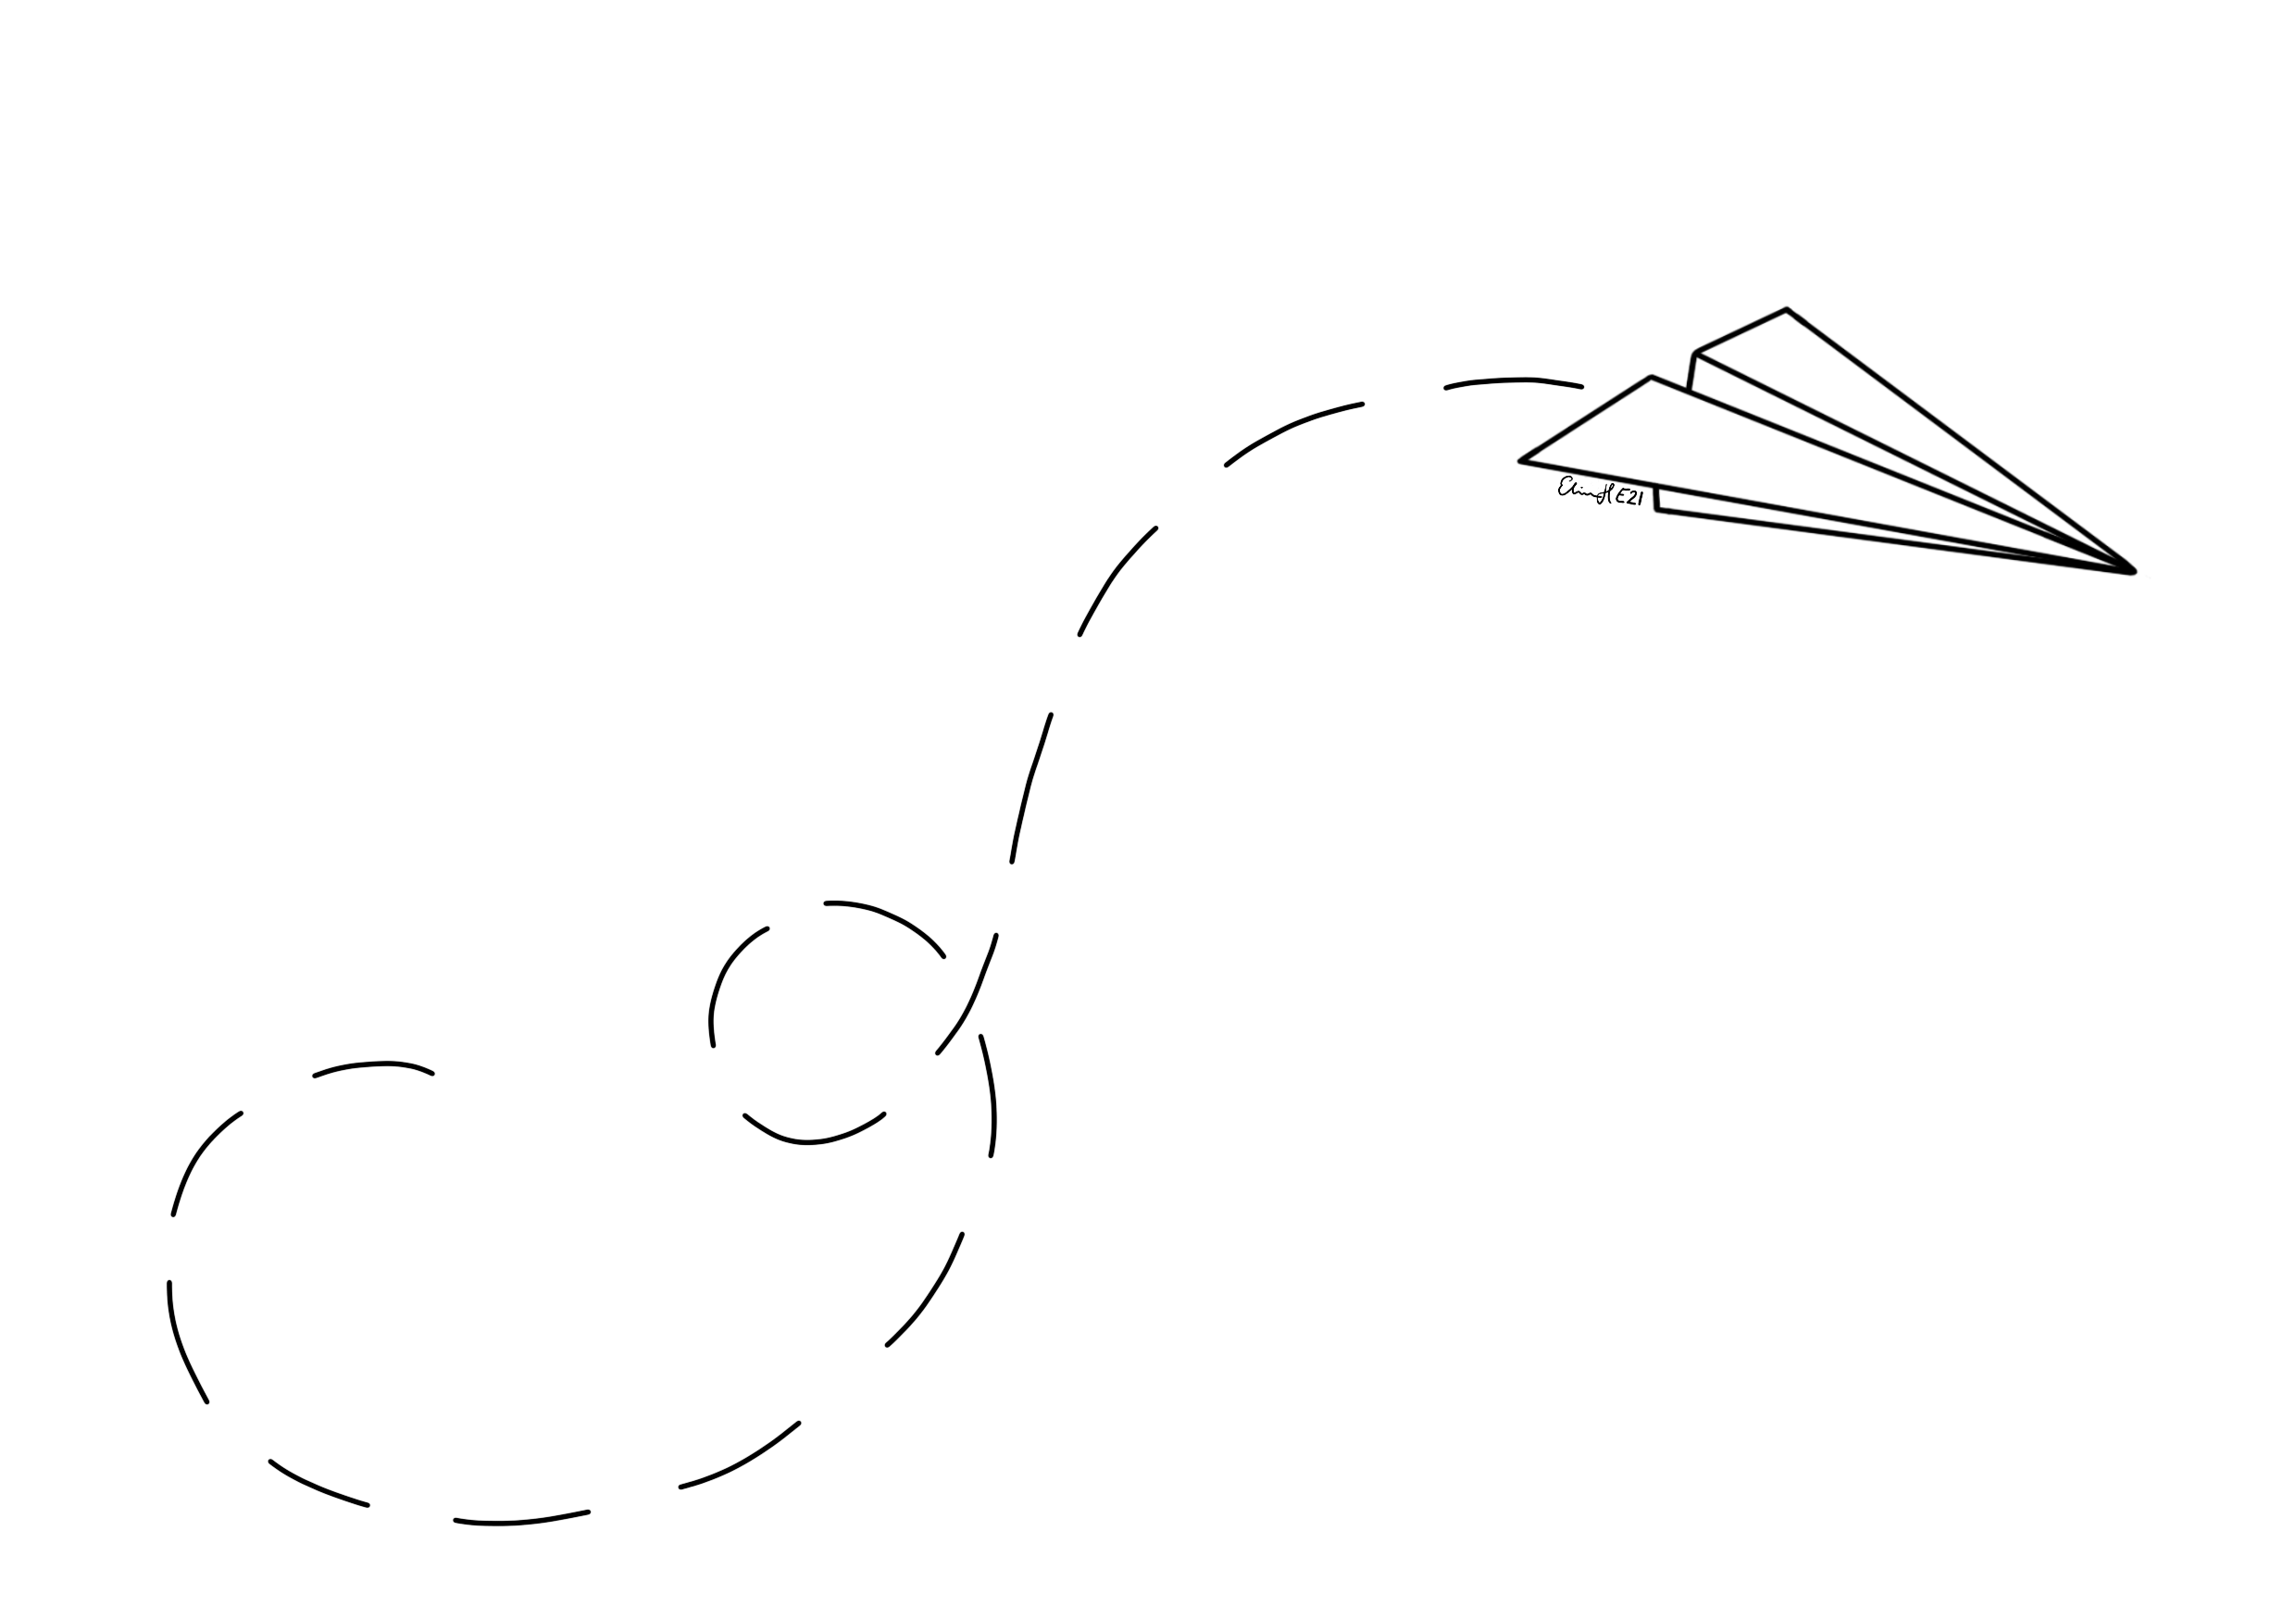
\includegraphics[width=20cm]{./bilder/pappersplan_signerad.png}
\end{textblock*}

\vspace*{5cm}
\subsection*{Röda havet} 
\index[alfa]{Röda havet}
\index[anfa]{Vi gingo ner till Röda havet}
\songinfo{Mel: Skrattvisa ur Orfeus i underjorden \\(Pour séduire Alcmène a la fière)}

\begin{parse lines}[\noindent]{#1\\}
    Vi gingo ned till Röda havet
    Vi lågo i där minst en kvart
    Ja, minst en kvart
    Men inte blev vi röda av 'et
    Men Röda havet det blev svart
    
    Men utav aqvavit
    Människan till kropp och själ
    Blir oskuldsfull och vit
    Men utav aqvavit
    Människan till kropp och själ
    Blir oskuldsfull och vit
\end{parse lines}

\newpage
\resetBackground

\subsection*{Stadsparksdammen} 
\index[alfa]{stadsparksdammen}
\index[anfa]{Vi gingo ner till stadsparksdammen}
%\songinfo{}

\begin{parse lines}[\noindent]{#1\\}

    Vi gingo ner till stadsparksdammen
    Vi lågo i där minst en kvart
    Ja, minst en kvart
    Men inte blev vi av med skammen
    Men stadsparksdammen den blev svart
    
    Men utav aqvavit…

\end{parse lines}

\subsection*{Lommabukten} 
\index[alfa]{Lommabukten}
\index[anfa]{Vi gingo ned till Lommabukten}
%\songinfo{}

\begin{parse lines}[\noindent]{#1\\}

    Vi gingo ned till Lommabukten
    Vi lågo i där minst en kvart
    Ja, minst en kvart.
    Men inte blev vi av med lukten
    Men Lommabukten den blev svart
    
    Men utav aqvavit...
\end{parse lines}

\newpage

\subsection*{Finska viken} 
\index[alfa]{Finska viken}
\index[anfa]{Vi gingo ner till Finska viken}
%\songinfo{}

\begin{parse lines}[\noindent]{#1\\}

    Vi gingo ner till Finska viken
    Vi lågo i där minst en kvart
    Ja, minst en kvart
    Men inte blev vi av med skiten
    men Finska viken den blev svart
    
    Men utav aqvavit…

\end{parse lines}

\subsection*{Systembolaget} 
\index[alfa]{Systembolaget}
\index[anfa]{Vi gingo ner till Systembolaget}
%\songinfo{}

\begin{parse lines}[\noindent]{#1\\}

    Vi gingo ner till Systembolaget
    Vi stod i kö där minst en kvart
    Ja, minst en kvart
    Men inte blev vi fulla av det
    Systembolaget det gick back
    
    Men utav aqvavit…
\end{parse lines}

\vissteduatt{Visste du att Aqvavit = aqua vitae = livets vatten?}
\newpage

\subsection*{Labblokalen} 
\index[alfa]{Labblokalen}
\index[anfa]{Vi gingo ned till labblokalen}
%\songinfo{}

\begin{parse lines}[\noindent]{#1\\}

    Vi gingo ned till labblokalen
    Vi var där inne minst en kvart
    Ja, minst en kvart.
    Men inte blev vi av med kvalen
    Men labblokalen den blev svart
    
    Men utav aqvavit...
\end{parse lines}

\subsection*{Vi gingo ner till Edekvata} 
\index[alfa]{Vi gingo ner till Edekvata}
\index[anfa]{Vi gingo ner till Edekvata}
%\songinfo{}

\begin{parse lines}[\noindent]{#1\\}

    Vi gingo ner till Edekvata
    Vi olja borden minst en kvart
    Ja, minst en kvart
    Men manualen den vi rata
    så Edekvata det blev svart
    
    Men utav aqvavit…
    
\end{parse lines}

\vissteduatt{Visste du att det brann i Edekvata 2010?
\\En trasa med linolja självantände...}
\newpage

\subsection*{Karnevalen} 
\index[alfa]{Karnevalen}
\index[anfa]{Vi gingo ner till karnevalen}
%\songinfo{}

\begin{parse lines}[\noindent]{#1\\}
    
    Vi gingo ner till karnevalen
    Och stod i kö där minst en kvart
    Ja, minst en kvart
    Vi ville in i AF-salen
    Men inte fan kom vi nå'n vart

    För utav kösystem
    Blir det bara skit och massa allmänna problem
    För utav kösystem
    Blir det bara skit och massa allmänna problem
    
    Och vi kom fram till kravallstaketet
    Och stod kvar där minst en kvart
    Ja, minst en kvart
    Sen vi var fast i köhelvetet
    Så inte fan kom vi nå'n vart
    
    För utav kösystem…
    
\end{parse lines}


\newpage


%\begin{center}
    \vspace*{1.5cm}
    {\fontsize{20}{20}\textbf{Slaskvisor}}\\
    \vspace{0.7cm}
    {\fontsize{12}{12}\textit{Om ... själv får välja}}
\end{center}
\addtocwithheader{Slaskvisor}  % Add entry to TOC and set header\noBackground
\noBackground

\newpage
\noBackground

% ----- GAMLA BAMSE -----
%\begin{textblock*}{3cm}(6.0cm,2.5cm) % {width}(x, y)
%    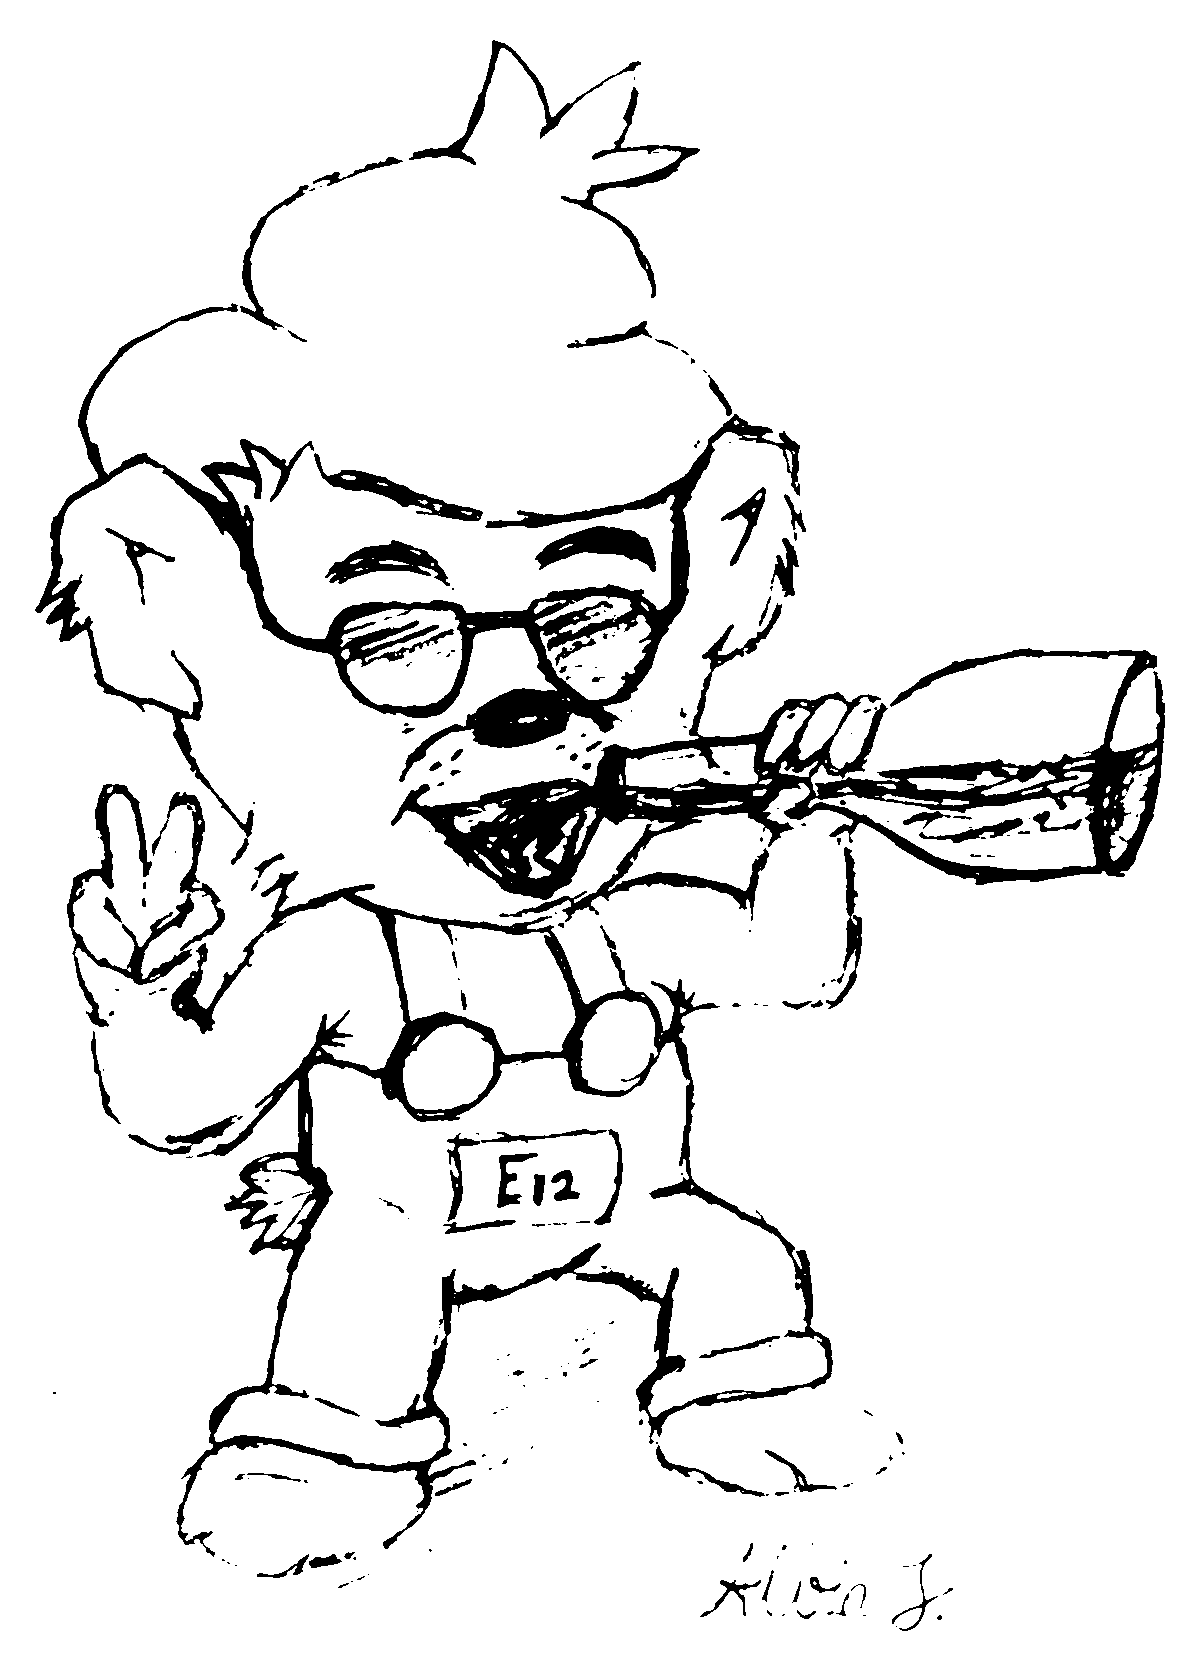
\includegraphics[width=4.7cm]{./bilder/bamse.png}
%\end{textblock*}

% ----- NYA BAMSE -----
\begin{comment}
\begin{textblock*}{3cm}(5.5cm,3.2cm) % {width}(x, y)
    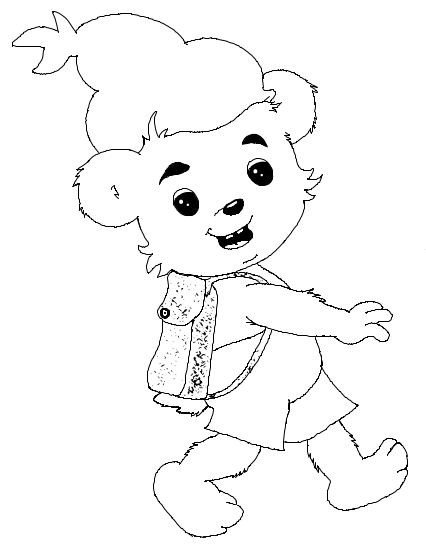
\includegraphics[width=2.8cm]{./bilder/majas-bilder/bamse-1.png}
\end{textblock*}

\begin{textblock*}{3cm}(7.6cm,6.7cm) % {width}(x, y)
    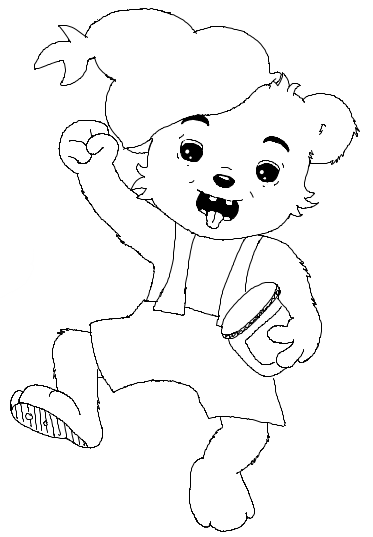
\includegraphics[width=2.6cm]{./bilder/majas-bilder/bamse-2.png}
\end{textblock*}

\begin{textblock*}{3cm}(5.6cm,10.2cm) % {width}(x, y)
    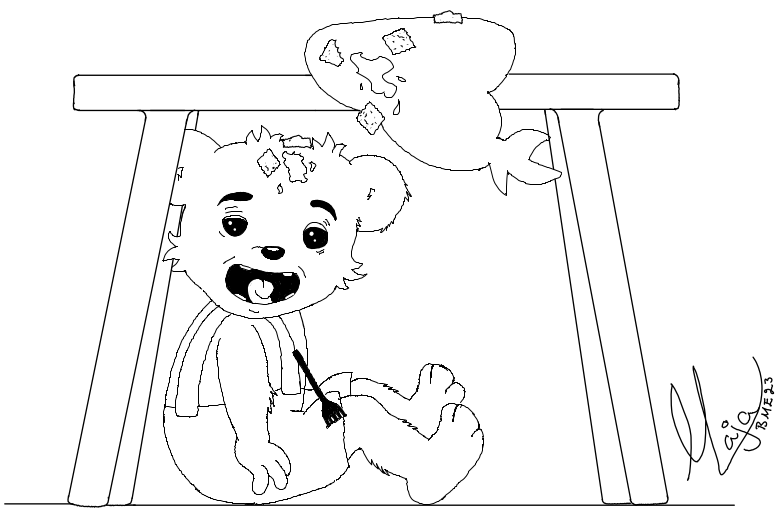
\includegraphics[width=4.9cm]{./bilder/majas-bilder/bamse-3.png}
\end{textblock*}


\begin{textblock*}{3cm}(7cm,2cm) % {width}(x, y)
    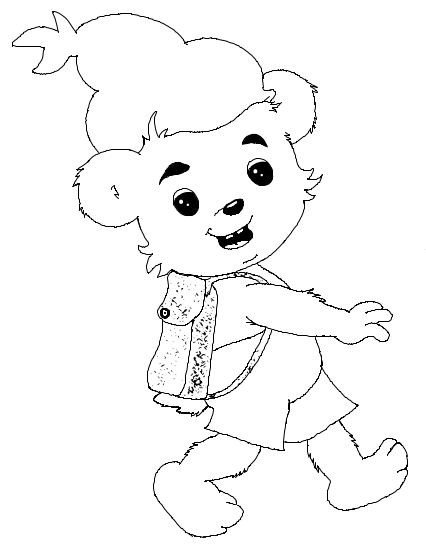
\includegraphics[width=3.2cm]{./bilder/majas-bilder/bamse-1.png}
\end{textblock*}

\begin{textblock*}{3cm}(6 cm,5.5cm) % {width}(x, y)
    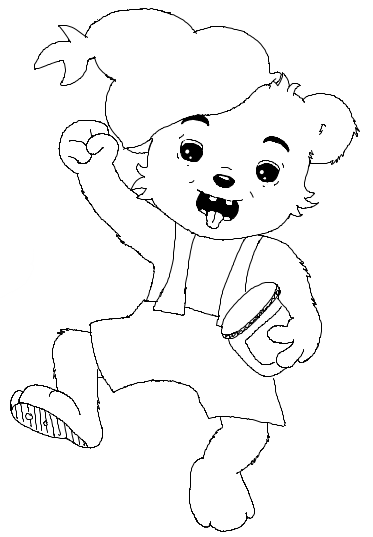
\includegraphics[width=2.8cm]{./bilder/majas-bilder/bamse-2.png}
\end{textblock*}

\begin{textblock*}{3cm}(6cm,9.4cm) % {width}(x, y)
    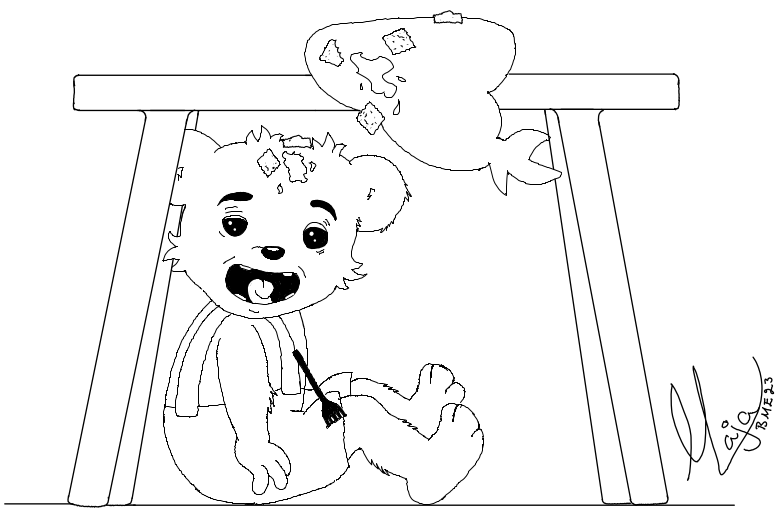
\includegraphics[width=4.9cm]{./bilder/majas-bilder/bamse-3.png}
\end{textblock*}


\begin{textblock*}{3cm}(7.6 cm, 3.2cm) % {width}(x, y)
    %\scalebox{-1}[1]{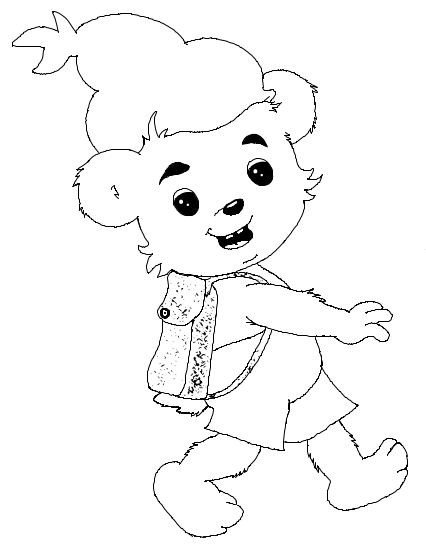
\includegraphics[width=2.4cm]{./bilder/majas-bilder/bamse-1.png}}
    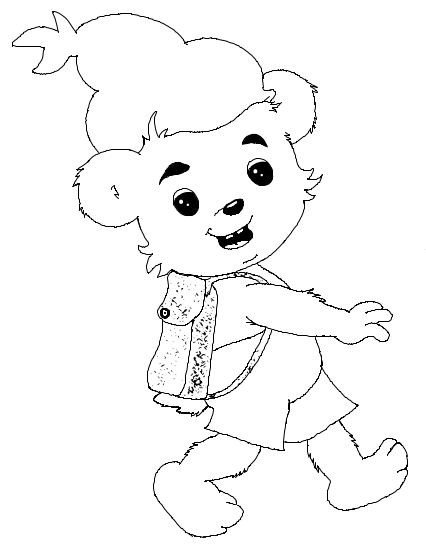
\includegraphics[width=2.4cm]{./bilder/majas-bilder/bamse-1.png}
\end{textblock*}

\begin{textblock*}{3cm}(6.6cm, 6cm) % {width}(x, y)
    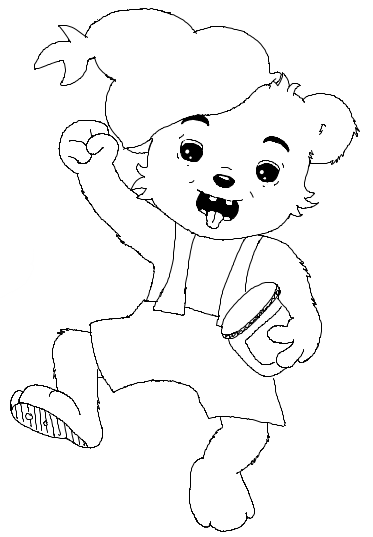
\includegraphics[width=2.2cm]{./bilder/majas-bilder/bamse-2.png}
\end{textblock*}

\begin{textblock*}{3cm}(6.6cm,9.3cm) % {width}(x, y)
    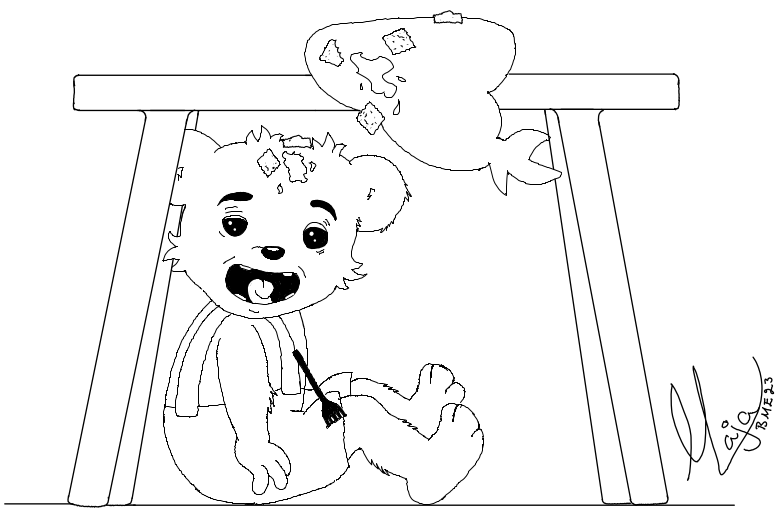
\includegraphics[width=3.8cm]{./bilder/majas-bilder/bamse-3.png}
\end{textblock*}
\end{comment}

\begin{textblock*}{3cm}(6.2cm,2.8cm) % {width}(x, y)
    \scalebox{-1}[1]{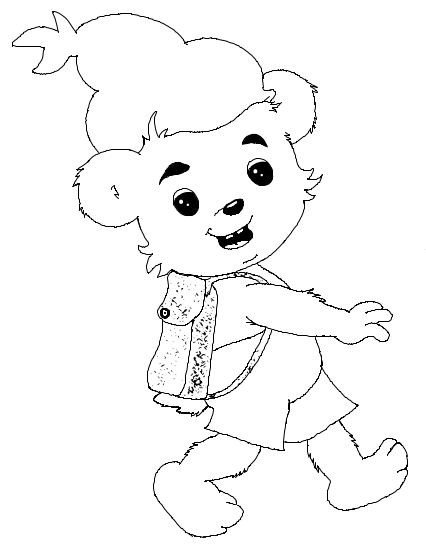
\includegraphics[width=2.7cm]{./bilder/majas-bilder/bamse-1.png}}
    %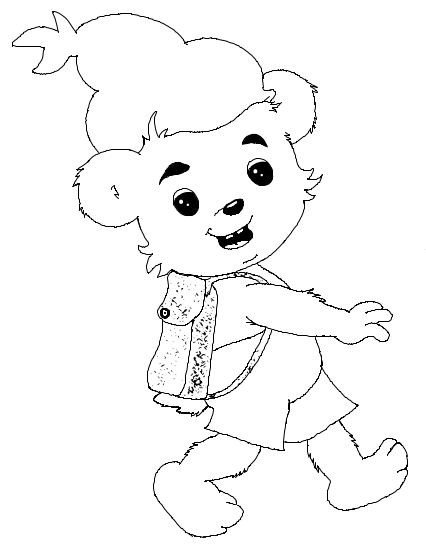
\includegraphics[width=2.4cm]{./bilder/majas-bilder/bamse-1.png}
\end{textblock*}

\begin{textblock*}{3cm}(7.5cm, 6.5cm) % {width}(x, y)
    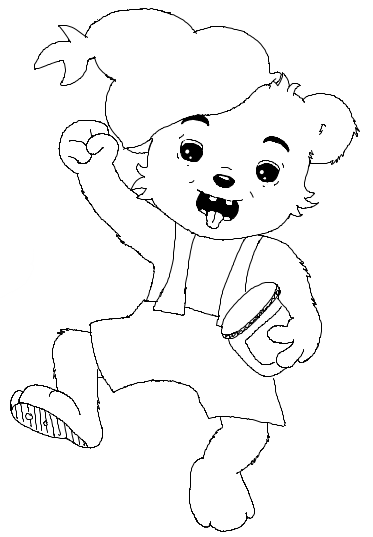
\includegraphics[width=2.4cm]{./bilder/majas-bilder/bamse-2.png}
\end{textblock*}

\begin{textblock*}{3cm}(5.7cm,10.3cm) % {width}(x, y)
    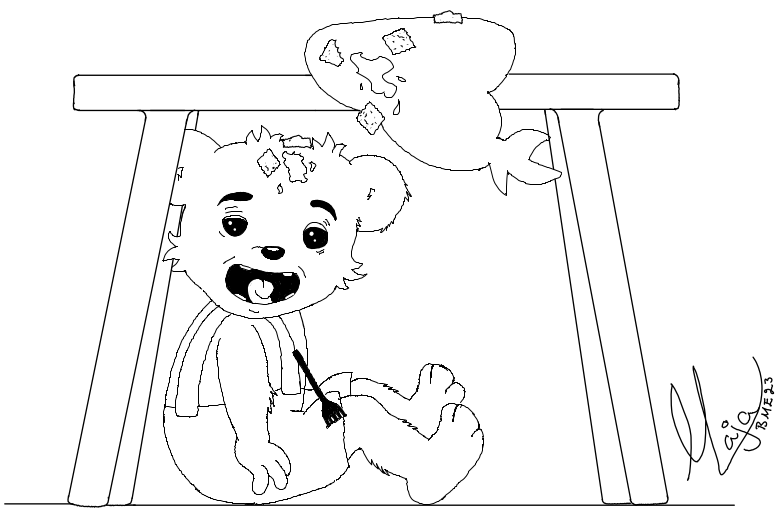
\includegraphics[width=4.2cm]{./bilder/majas-bilder/bamse-3.png}
\end{textblock*}

\subsection*{Jag skall festa} 
\index[alfa]{Jag skall festa}
\index[anfa]{Jag skall festa}
\songinfo{Mel: Bamse\\
Sångarstriden 1987}

\begin{parse lines}[\noindent]{#1\\}
    Jag ska festa, ta det lugnt med spriten,
    ha det roligt utan å va' full
    Inte krypa runt med festeliten,
    ta det varligt för min egen skull

    Först en öl i torra strupen,
    efter det så kommer supen,
    i med vinet, ner med punschen
    Sist en groggbuffé

    Jag är skitfull, däckar först av alla,
    missar festen, men vad gör väl de'?
    Blandar hejdlöst öl och gammal filmjölk,
    kastar upp på bordsdamen breve'!

    Först en öl... 

    Spyan rinner ner för ylleslipsen
    Raviolin torkar i mitt hår
    Vem har lagt mig under matsalsbordet?
    Vems är gaffeln i mitt högra lår?
\end{parse lines}

\vissteduatt{Visste du att denna sången tillsammans med Vikingen var de\\första sångerna som lades in i denna upplagan av sångboken?}

\newpage
\resetBackground

\subsection*{Ångestvisan} 
\index[alfa]{Ångestvisan}
\index[anfa]{Ångestvisan}
\songinfo{Mel: Mössens julafton}

% \colorbox{yellow}{OSÄKER PÅ DENNA}

\begin{parse lines}[\noindent]{#1\\}
    Jag vaknar upp på söndan
    och bakis som ett djur
    så kommer minnen om att gårdagskvällen spårat ur
    Jag blev visst lite busig av humle och av malt,
    på snapchatstoryn har jag publicerat allt

    Fan då, jävlar, bakfyllepanik!
    För storyn min har blivit till en eländesfabrik
    Fan då, jävlar vad ska jag ta mig till?
    För allt där finns ju sparat vare sig jag vill!

    Jag hångla med min granne
    och fast det ej va rätt,
    så sålde jag hans möbler och hans katt på internet
    Jag känner mig så rutten, jag är så full av skam
    Av alla jävla bilder på min instagram!

    Fan då, jävlar…

    Jag badade i sjön Sjøn?
    och till min stora skräck,
    så fick en barnfamilj bevittna när jag dansa näck
    Jag ramlade in i bastun, och spydde upp all gin
    och likea alla exets bilder på LinkedIn

    Fan då, jävlar…
\end{parse lines}

\newpage

\subsection*{Jesus lever} 
\index[alfa]{Jesus lever}
\index[anfa]{Jesus lever}
\songinfo{Mel: Sån’t är livet}

\begin{parse lines}[\noindent]{#1\\}
    Jesus lever, han bor i Skövde
    Han kör en Volvo och han är gift
    Han har en villa med rododendron
    Han sparar pengar och jobbar skift

    Redan på lekis var han märklig
    Han ville inte leka krig
    Men när hans kompis, Knut, blev skjuten
    så lät han Jesus uppväcka sig

    Jesus lever, han bor i Skövde...

    Han gick i skolan, som alla andra
    Han var rätt duktig på gymnastik
    å vilken kille han gick på vatten
    en gång så gick han till Reykjavik

    Jesus lever, han bor i Skövde...

    I sina tonår så var han poppis
    Och han blev bjuden på varje fest
    Å vilken kille, han fick ju vatten
    att bli till rusdryck utan jäst

    Jesus lever, han bor i Skövde...
\end{parse lines}

\vissteduatt{Visste du att E-sektionen har en egen E-wiki?}
\newpage

\subsection*{Fyllevisa} 
\index[alfa]{Fyllevisa}
\index[anfa]{Jesus lever}
\songinfo{Mel: Vi går över daggstänkta berg}
\begin{parse lines}[\noindent]{#1\\}
    Vi som oss för att glupa satt, supa glatt,
    ity den, som försmår sin första tår, törsta får
    Av längtan vi tryckas
    av trängtan att lyckas
    Vi nu med bravur häller ur,
    eller hur?

    Vi ger titt som tätt strupen sitt: Supen stritt
    skall forsa, och snart får sig tarmen vår, varm en tår
    Er öven i seder
    och söven er neder
    vid denna protest-bullerfest:
    Full är bäst!
\end{parse lines}


\newpage

\subsection*{Mat och vin och öl och sprit} 
\index[alfa]{Mat och vin och öl och sprit}
\index[anfa]{Mat och vin och öl och sprit}
\songinfo{Mel: She’ll Be Coming ‘Round the Mountain\\
F-sektionen Sångarstriden 07/08}

\noindent Mat och vin och öl och sprit serveras här,\\
\noindent teknologer lider inte av misär\\
\noindent Fatta glasen och höj hatten,\\
\noindent drick nu upp den sista slatten\\
\noindent Mera vin och öl och sprit det kommer här!\\

\noindent \textit{Trula:}\\
\noindent Bordsherren min han verkar ganska snäll, \textit{(Jättesnäll!)}\\
\noindent men han beter sig lite underligt ikväll \textit{(Just ikväll!)}\\
\noindent När han glufsar i sig maten,\\
\noindent rapar högt och krossar faten\\
\noindent Tafsar han på mig då får han sig en smäll!\\

\noindent \textit{Truls:}\\
\noindent Bordsdamen min är faktiskt riktigt grann, \textit{(Jättegrann!)}\\
\noindent men hon halsar i sig ölen som en man \textit{(Vilken man?!)}\\
\noindent Vinglar hon så välter stolen,\\
\noindent Shakear loss och tappar kjolen\\
\noindent Bäst att låtsas att vi inte känt varann!\\

\noindent Mat och vin och öl och sprit serveras här...\\

\vissteduatt{Visste du att vid höstterminsmötet 2013 höll E-sektionen på att köpa\\en Zamboni?}

\newpage

\subsection*{Man kan dricka vatten} 
\index[alfa]{Man kan dricka vatten}
\index[anfa]{Man kan dricka vatten}
\songinfo{Mel: Vi äro musikanter}

\begin{parse lines}[\noindent]{#1\\}
    Man kan dricka vatten, mjölk och gammalt flott
    Men vi dricker hellre sådant som är gott

    Vi kan dricka brännvin, öl och billigt vin
    Vi kan dricka olja och bensin

    Och vi kan svepa islandshästar, mockavästar när vi festar
    Vi kan svepa svavelsyra på vår yra fest

    Vi kan häva kvicksilver och helium
    Vi kan häva ost och vardagsrum

    Och vi kan supa bomfadderalla, bomfadderalla,
    skål på Er alla!
    Vi kan supa andra hållet, andra hållet med
\end{parse lines}

\vissteduatt{Visste du att denna sångbok är skriven i \LaTeX?}

\newpage

\subsection*{Baklängesfyllan} 
\index[alfa]{Baklängesfyllan}
\index[anfa]{Baklängesfyllan}
\songinfo{Mel: Rövarnas visa\\
Lundakarnevalen 2018}

\begin{parse lines}[\noindent]{#1\\}
    Jag hulkar mig i spyorna
    Och sedan med en gaffel
    Ur munnen min jag plockar fram
    En extra stor falafel
    
    Sen baklänges jag vinglar bord
    Till efterfest av bästa sort
    Jag spottar ut shot, efter shot, efter shot
    ja så här finemang har jag aldrig mått!
    
    (Å shot, shot, shot, shot. Å shot, shot, shot, shot.)
    
    Till Lundagård jag rullar sen 
    Och ställer någons cykel
    På klubbens dansgolv hittar jag
    Min plånbok och min nyckel
    
    Fem öl, sju snaps, en flaska vin
    Jag häller upp ur halsen min
    Ikväll ska jag plugga det lovar jag dig,
    men en endaste öl kan man unna sig!
    
\end{parse lines}

\newpage


\begin{textblock*}{3cm}(8.5cm,-0.7cm) % {width}(x, y)
    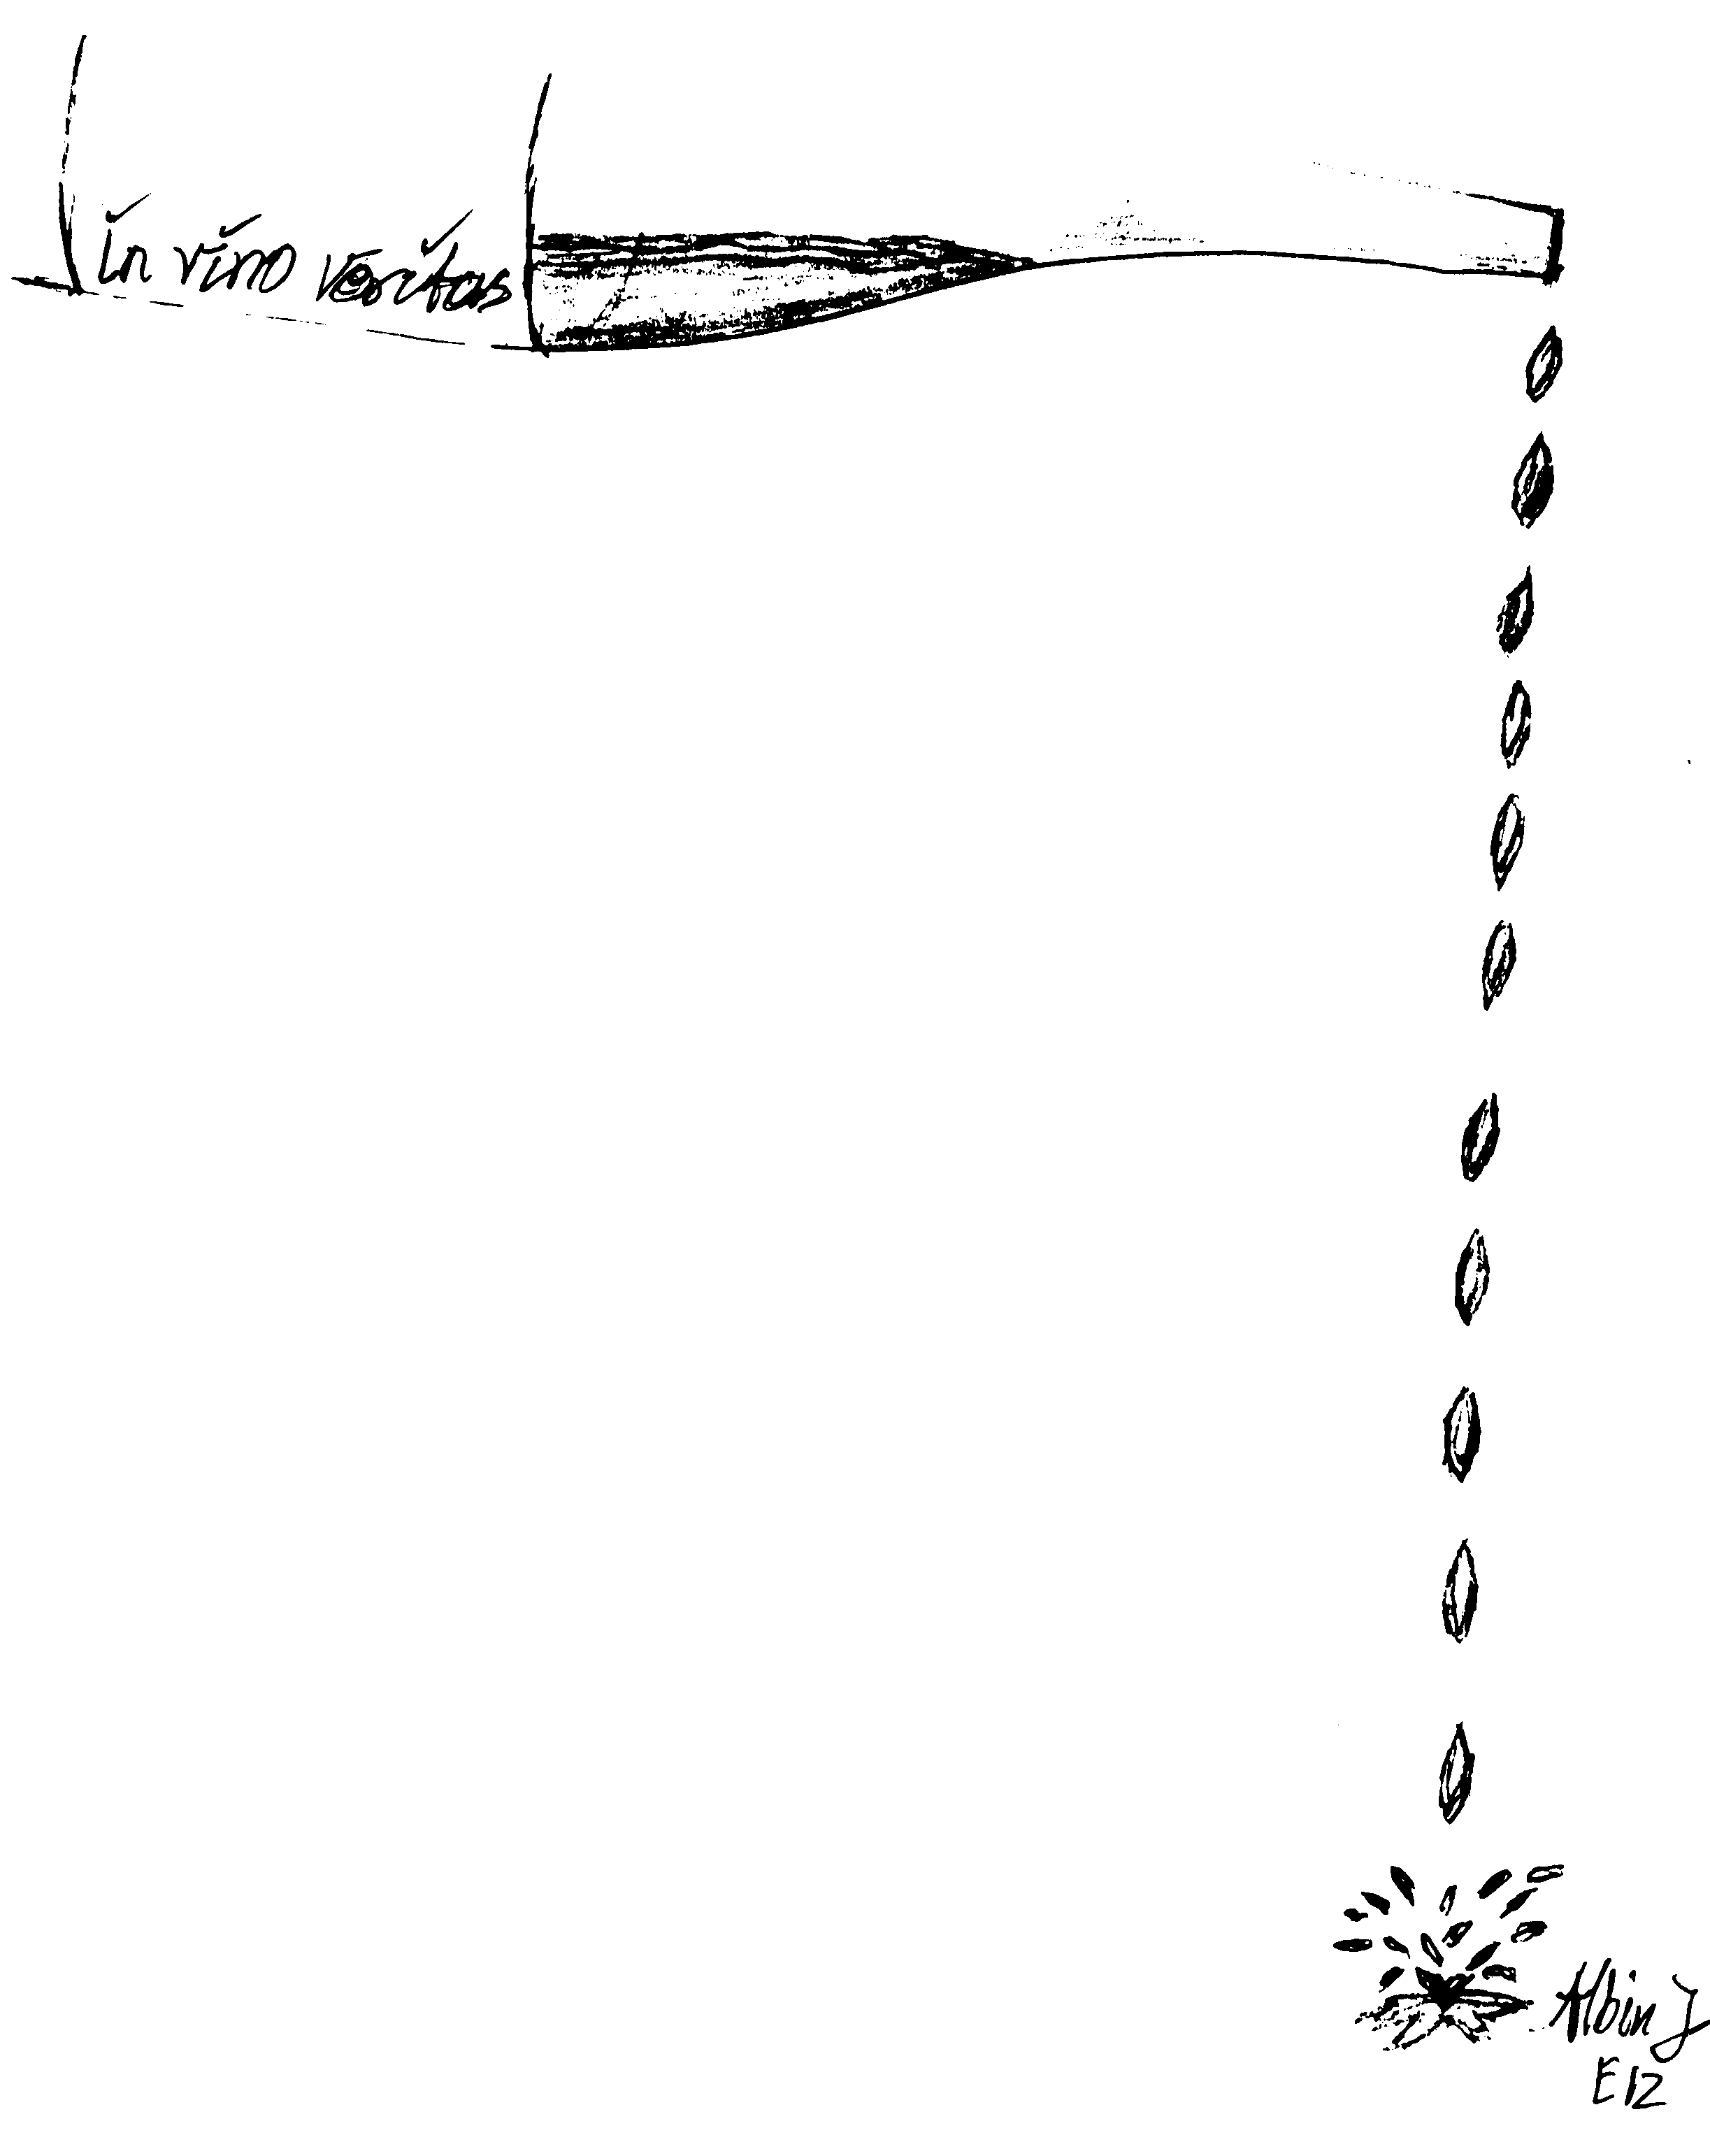
\includegraphics[width=12cm]{./bilder/in_vino_veritas.png}
\end{textblock*}

\subsection*{Kalmarevisan} 
\index[alfa]{Kalmarevisan}
\index[anfa]{Uti Kalmare stad}
\songinfo{Sången leds av sångförman}

\noindent \textit{Uti Kalmare stad,} \\
\noindent ja där finns det ingen kvast \\
\noindent förrän lördagen \\

\noindent \textit{Hej dick,} hej dack\\
\noindent \textit{Jag slog i,} och vi drack\\
\noindent \textit{Hej dickom dickom dack,}\\
\noindent Hej dickom dickom dack\\
\noindent För uti Kalmare stad\\
\noindent ja där finns det ingen kvast\\
\noindent förrän lördagen\\

\noindent ||: \textit{När som bonden kommer hem}\\
\noindent kommer bondegumman ut :||\\
\noindent är så stor i sin trut\\
\noindent \textit{Hej dick…}\\

\noindent ||: \textit{Var är pengarna du fått?}\\
\noindent - Jo, dem har jag supit opp :||\\
\noindent uppå Kalmare slott\\
\noindent \textit{Hej dick…}\\

\vissteduatt{Visste du att LTH-fontänen invigdes 1970 men plockades ner 1996\\efter otaliga försök att reparera den? Kvar står stålskelettet.}

\newpage

\begin{textblock*}{3cm}(-2.0cm,-0.7cm) % {width}(x, y)
    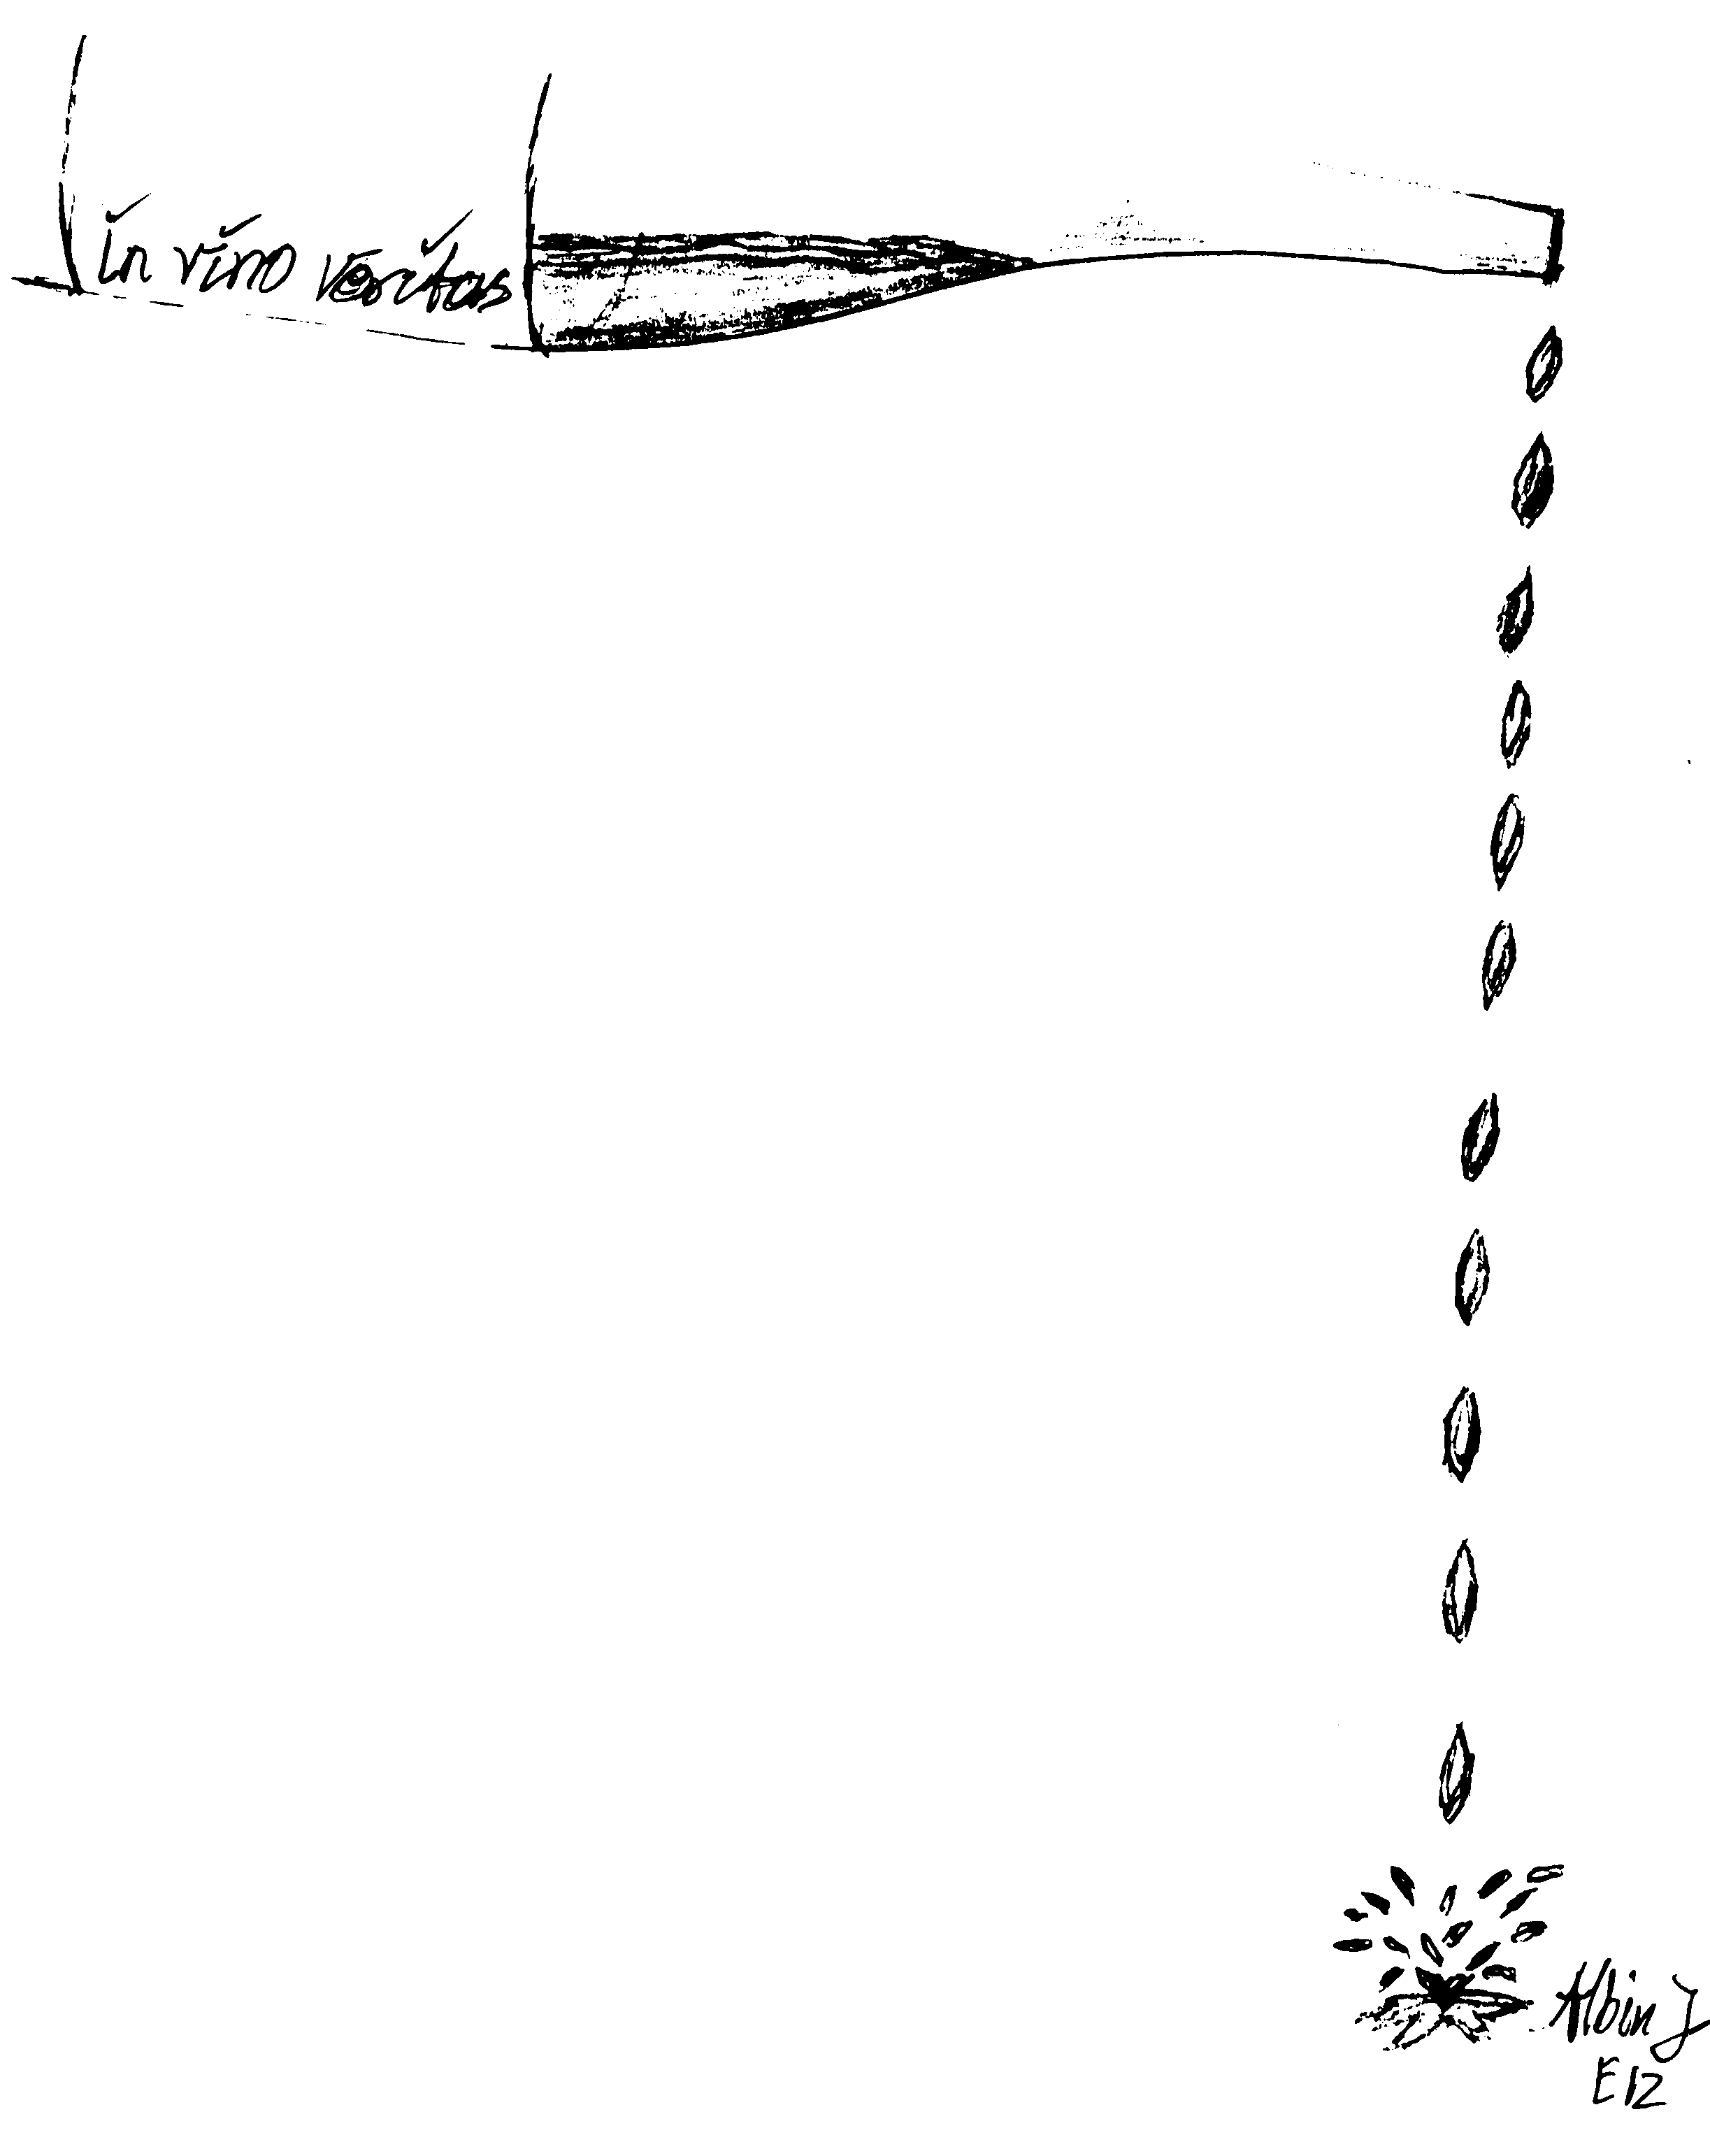
\includegraphics[width=12cm]{./bilder/in_vino_veritas.png}
\end{textblock*}

*\vspace{1cm}

\noindent ||: \textit{Jag skall klaga dig an}\\
\noindent för vår kronbefallningsman :||\\
\noindent och så får du skam\\
\noindent \textit{Hej dick…}\\

\noindent ||: \textit{Kronbefallningsmannen vår}\\
\noindent satt på krogen i går :||\\
\noindent och var full som ett får\\
\noindent \textit{Hej dick…}\\

\noindent ||: \textit{Var har du din labbrapport?}\\
\noindent Jo den har jag supit bort! :||\\
\noindent Den var allt för kort\\
\noindent \textit{Hej dick…}\\

\vissteduatt{Visste du att "In Vino Veritas"?}

\newpage

\subsection*{Spritbolaget} 
\index[alfa]{Spritbolaget}
\index[anfa]{Till spritbolaget ränner jag}
\songinfo{Mel: Snickerboa\\
Text: Göran Bolinder\\
E-sektionen Sångarstriden 1989}

\begin{parse lines}[\noindent]{#1\\}
    Till spritbolaget ränner jag
    och bankar på dess port
    Jag vill ha nå't som bränner bra
    och gör mig sketfull fort
    Expediten sade: Godda',
    hur gammal kan min herre va'?
    Har du nå't leg, ditt fula drägg?
    Kom hit igen när du fått skägg!
    
    Nej, detta var ju inte bra,
    jag ska bli full ikväll
    Då plötsligt en idé fick jag:
    De har ju sprit på Shell
    Många flaskor stod där på rad,
    så nu kan jag bli full och glad
    Den röda drycken åkte ner...
    Nu kan jag inte se nå't mer
\end{parse lines}

\vissteduatt{Visste du att E-sektionen har den längsta svansen i hela Världen?\\Visste du att E-sektionen bara kom på andra plats med Spritbolaget?}

\newpage


\subsection*{Härjarevisan} 
\index[alfa]{Härjarevisan}
\index[anfa]{Nu ska vi ut och härja}
\songinfo{Mel: Gärdebylåten\\ Ur Lundaspexet Djingis Khan 1954\\ Text: Hans Alfredsson}

\begin{parse lines}[\noindent]{#1\\}
    Hurra! Nu ska man äntligen få röra på benen
    Hela stammen jublar och det spritter i grenen
    Tänk att än en gång få spränga fram på Brunte i galopp!
    Din doft, o käre Brunte är trots brist i hygienen,
    för en vild mongol minst lika ljuv som syrenen
    Tänk att på din rygg få rida runt i sta'n och spela topp!

    Ja, nu ska vi ut och härja,
    supa och slåss och svärja,
    bränna röda stugor, å' så lära små barn fula ord
    Med blod ska vi stäppen färga
    Nu änteligen lär jag
    kunna dra nån verklig nytta av min
    hermodskurs i mord

    För mordbränder är härliga, ta hit fotogenen
    Eftersläckningen tillhör just de fenomenen
    inom brandmansyrket som jag tycker det är nån nytta med
    Jag målar för mitt inre upp den härliga scenen,
    blodrött mitt i brandgult, ej prins Eugen en
    lika mustig vy kan måla, ens om han målade med sked

    Ja, nu ska vi ut och härja…

\end{parse lines}

\vissteduatt{Visste du att det finns en tredje vers som felaktigt sjunges av andra\\högskolor innan första versen? Originalet skrevs trots allt i Lund...}

\newpage

\subsection*{Smögen} 
\index[alfa]{Smögen}
\index[anfa]{Kärlek och solsken och sång}
\songinfo{Mel: När jag var en ung caballero}
\begin{parse lines}[\noindent]{#1\\}
    När jag vart’ och spytt på kalaset 
    Så kallar dom mig fylle-..........Karlsson 
    En Karlsson för kärlek och solsken och sång, 
    för kärlek och solsken och sång, PLING PLONG 
    
    Så ramla jag på någon Trula 
    Och vi börja genast att .......... prata 
    Prata för kärlek… 
    
    Hon sade att hon hette Ulla 
    och fråga om vi skulle .......... dansa 
    
    Hon ville att jag ville titta 
    på hennes förtjusande .......... våning 
    En våning för kärlek… 
    
    Hon ville att jag ville titta 
    på hennes förtjusande .......... våning 
    En våning för kärlek… 
    
    Hon sa: “Här é vackert om hösten” 
    och smekte de fylliga .......... bolstren 
    Det var bolster för kärlek… 
    
    Som förrätt, hon sa “får väl duga 
    att vi varann häftigt kan .......... krama” 
    Det var kramar för kärlek… 
\end{parse lines}

\newpage
\noBackground

\begin{textblock*}{3cm}(1cm,10.4cm) % {width}(x, y)
    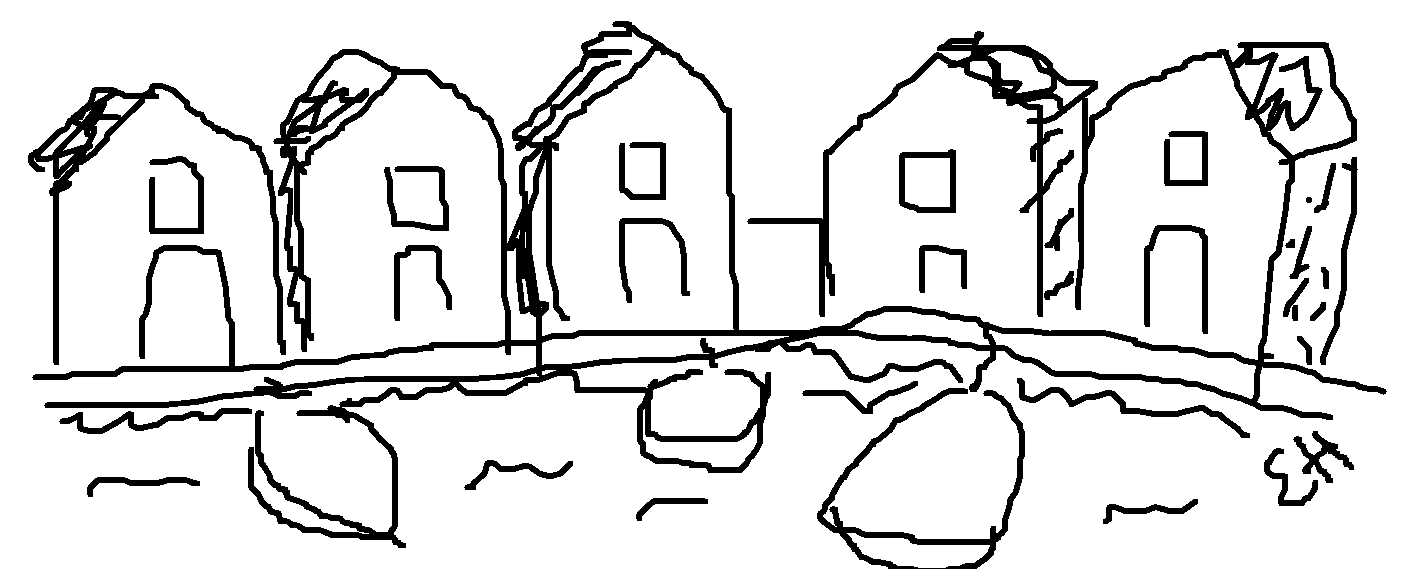
\includegraphics[width=8.5cm]{./bilder/smogen.png}
\end{textblock*}

\begin{parse lines}[\noindent]{#1\\}
    Hon bjöd mig på kaffe och tårta 
    och vi blev så helvetes .......... mätta 
    Vi va mätta på kärlek… 
    
    Så spillde jag kaffe på duken 
    jag torkade upp det med .......... trasan 
    En trasa för kärlek… 
    
    Då kom hennes storebror Östen 
    Han bad henne visa mig .......... tavlan 
    En tavla för kärlek… 
    
    Så tog hon av sig till mitten, 
    och jag börja fumla med .......... TVn 
    En TV för kärlek… 
    
    Sen börja vi ekorrar härma 
    när jag fyllde henne med .......... nötter 
    Det var nötter för kärlek… 
    
    Sen börja jag hemåt att lunka 
    Jag stanna i porten och .......... gäspa 
    Jag gäspa för kärlek…

\end{parse lines}
\vissteduatt{\\Visste du att den här bilden ritades på 2 minuter i MS Paint}
\newpage
\resetBackground

\subsection*{Antisnapsvisa} 
\index[alfa]{Antisnapsvisa}
\index[anfa]{Huvudet vi lyfter med ett stön ur vår säng}
\songinfo{Mel: Sjösala vals}

\begin{parse lines}[\noindent]{#1\\}
    Huvudet vi lyfter med ett stön ur vår säng,
    tvättmaskin i buken, kanoner i huvudet.
    Tungan som en plyschsoffa och yrseln i sväng,
    i ångesten vi svettas 
    kom sjung din refräng:

    Varför finns det aldrig nå'n nykter karneval?
    O, låt oss somna om så vi slipper våra kval
    men se så många supar vi redan kastat upp i sängen:
    Renat och Skåne, Svart Vinbär och fager Bäsk
\end{parse lines}

\subsection*{Katastrofalt uppvaknande} 
\index[alfa]{Katastrofalt uppvaknande}
\index[anfa]{Jag vaknade i stolen}
\songinfo{Mel: Stad i ljus\\
Lundakarnevalen 2022}

\begin{parse lines}[\noindent]{#1\\}
    Jag vaknade i stolen, har slumrat till här i mitt rum
    Och allting känns eländigt, mitt bord är fyllt med 
    flaskor - en har runnit ut
    Jag tror jag minns spektaklet och alla dom som 
    förde liv
    Konturen av ett party, jag hade efterfest som växte -
    blev massiv

    Jag är full!
    i ett kaosartat rum
    Ge mig frid
    så jag får somna om
\end{parse lines}

\vissteduatt{Visste du att vid höstterminsmötet 2021 höll E-sektionen på att köpa\\in en åkbar sopmaskin och bygga om halva Edekvata till garage?}
\newpage
\noBackground

\begin{textblock*}{3cm}(2.8cm,7.2cm) % {width}(x, y)
    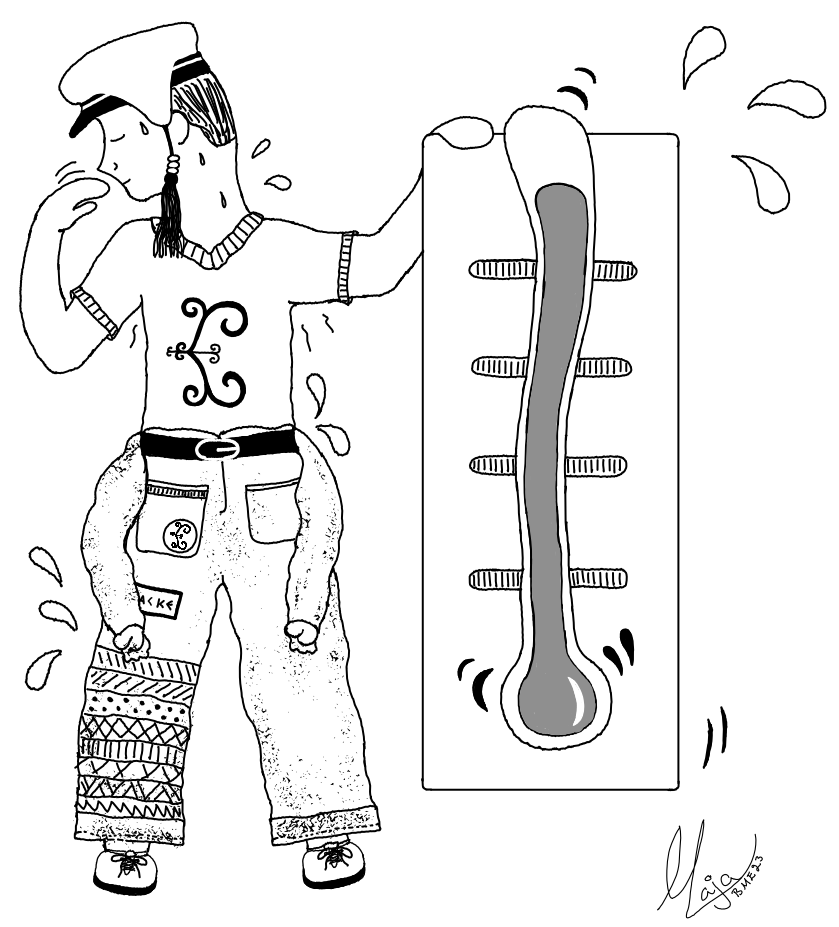
\includegraphics[width=6cm]{./bilder/majas-bilder/temperaturen.png}
\end{textblock*}

\subsection*{Temperaturen} 
\index[alfa]{Temperaturen}
\index[anfa]{Temperaturen}
\songinfo{Text: Mora Träsk}

\begin{parse lines}[\noindent]{#1\\}
    När temperaturen är hög uti kroppen
    Närmare 40 än trettiosju komma fem
    Så ska det vara när ångan är uppe
    och så är fallet uti detta nu

    Vi rullar, vi rullar…

    August och Lotta…

    Framåt och bakåt…

    ...
\end{parse lines}

\newpage

% \begin{center}
    \vspace*{1.5cm}
    {\fontsize{20}{20}\textbf{Punschvisor}}\\
    \vspace{0.7cm}
    {\fontsize{12}{12}\textit{Om sötsuget själv får välja}}
\end{center}
\addcontentsline{toc}{section}{Punschvisor}
\noBackground

\newpage
\resetBackground

  
  \subsection*{Punschen kommer (kall)} 
  \index[alfa]{Punschen kommer (kall)}
  \index[anfa]{Punschen kommer ljuv och sval}
  \songinfo{Mel: Vals ur Glada änkan}
  
  \begin{parse lines}[\noindent]{#1\\} 
    Punschen kommer, punschen kommer
    Ljuv och sval
    Glasen imma, röster stimma
    I vår sal
    Skål för glada minnen
    Skål för varje vår
    Inga sorger finnas mer
    När punsch vi får
  \end{parse lines}

  \subsection*{Punschen kommer (varm)} 
  \index[alfa]{Punschen kommer (varm)}
  \index[anfa]{Punschen kommer god och varm}
  \songinfo{Mel: Vals ur Glada änkan}
  
  \begin{parse lines}[\noindent]{#1\\} 
    Punschen kommer, punschen kommer
    God och varm
    Vettet svinner, droppen rinner
    Ner i tarm
    Skål för glada minnen
    Dem vi snart ej ha
    Då ett par glas simmig punsch
    Vi hunnit ta
  \end{parse lines}
  
  \vissteduatt{Visste du att...}
  
  \newpage


  \subsection*{Djungelpunsch} 
  \index[alfa]{Djungelpunsch}
  \index[anfa]{Jag gillar alla tiders punsch}
  \songinfo{Mel: Var nöjd med allt som livet ger}
  
  \begin{parse lines}[\noindent]{#1\\}
    Jag gillar alla tiders punsch
    Punsch till frukost, punsch till lunch
    Punsch till förrätt, varmrätt och dessert
    Jag gillar punsch för vet du vad
    Rent kaffe gör ju ingen glad
    Nej, punsch för fulla muggar vill jag ha
    
    Med konjak du lockar
    Den bästa Renault
    Förlåt om jag chockar
    Och tar punsch ändå
    Och bjuder du någon förnäm likör 
    Så får du ursäkta, det kanske stör
    Men jag väljer hellre Grönstedts Blå
    En Cederlunds eller Flaggpunsch å
    Kanske har du ren Platin?
    
    Jag gillar punsch, så ge mig punsch
    Och jag är din
    (Ja, jag är din)
    För evigt din
    
  \end{parse lines}
  
  \vissteduatt{Visste du att...}
  
  \newpage

  \subsection*{\colorbox{orange}{Jag gillar punschen}} 
  \index[alfa]{Jag gillar punschen}
  \index[anfa]{Jag gillar, jag gillar punschen}
  \songinfo{Mel: Te Deum (Eurovision theme)}
  \begin{parse lines}[\noindent]{#1\\} 
    Jag gillar, jag gillar punschen
    Jag gillar den som punschen skapat har
    Jag gillar, jag gillar punschen
    Jag gillar punschen och dess far
  \end{parse lines}

  \subsection*{När kaffet är serverat} 
  \index[alfa]{När kaffet är serverat}
  \index[anfa]{När kaffet är serverat}
  \songinfo{Mel: Mössens julafton\\
  Sångarstriden 1987
  }
  
  \begin{parse lines}[\noindent]{#1\\} 
    När kaffet är serverat och maten tagit slut
    Och alla dom som blivit alltför fulla kastats ut
    Då vill vi ha ett nytt glas med något gult och kallt
    Som höjer och förbättrar vår promillehalt
    Arrak, etanol och sackaros
    Med salt och vatten blir
    Den bästa blandning som kan fås
    Söt och smetig, rent utav viskös
    En sexton, sjutton glas så blir du medvetslös
    
  \end{parse lines}
  
  \vissteduatt{Visste du att...}
  
  \newpage

  \subsection*{\colorbox{orange}{Jag gillar punschen}} 
  \newpage


  \subsection*{Kretsloppet} 
  \index[alfa]{Kretsloppet}
  \index[anfa]{Genom vår kropp, ända till snopp}
  \songinfo{Mel: Nu har vi ljus}
  
  \begin{parse lines}[\noindent]{#1\\} 
    Genom vår kropp, ända till snopp
    Punsch håller färgen
    Hopp, tralalala
    Kolla ditt kiss, ser du, jovisst, ser du, jovisst
    Samma gyllengula ädla vätska
    Samma dryck som nyss vår tunga läska
    Tralalala lalalalala lalalalala lalala
    
    Tar punschen slut, spar på ditt krut
    Skjut inte värden, hopp, tralalala
    Låt punschen gå varv nummer två, varv nummer två
    Två och två ni mot varandra ilar
    Snart i munnen punschen åter strilar
    Tralalala lalalalala lalalalala lalala    
  \end{parse lines}
  
  \vissteduatt{Visste du att...}
  
  \newpage

  \subsection*{Familjen Addams punsch} 
  \index[alfa]{Familjen Addams punsch}
  \index[anfa]{Vi vill ha punsch}
  \songinfo{}
  \begin{parse lines}[\noindent]{#1\\} 
    Vi vill ha punsch, \dag \dag
    Vi vill ha punsch, \dag \dag
    Vi vill ha punsch, vi vill ha punsch
    Vi vill ha punsch, \dag \dag
    
    När man vill festen liva
    Upp är det bra att kliva
    Omkring på bordets skiva
    Och klafsa runt i punsch
    
    Klafsa i punsch, \ddag \ddag
    Klafsa i punsch, \ddag \ddag
    Klafsa i punsch, klafsa i punsch
    Klafsa i punsch, \ddag \ddag
    
  \end{parse lines}
  \noindent\textit{
    \\
    \dag = knäpp med fingrarna\\
    \ddag  = sörpla med munnen 
  }
  \vissteduatt{Visste du att...}
  
  \newpage

  \subsection*{\colorbox{orange}{Punschen vi radat} }
  \index[alfa]{Punschen vi radat}
  \index[anfa]{Punschen vi radat}
  \songinfo{Mel: Hemår detbär\\ \colorbox{yellow}{V-sektionen, Sångarstriden 1978???}\\ Kursivt sjunges av sångförman}
  
  \noindent Punschen vi radat upp på vårt bord\\
  Ädlare dryck ej finns på vår jord\\
  Hur härligt härlig du står och väntar på mig\\
  Oh, vad jag älskar dig!\\

  \noindent\textit{Oh, ljuva punsch\\}
  Oh, ljuva punsch\\

  \noindent\textit{Uti, min hand\\}
  Uti, min hand\\

  \noindent\textit{Nu tar du plats\\}
  Nu tar du plats\\

  \noindent\textit{I magens plats\\}
  I magens plats\\

  \noindent\textit{Jag drack dig upp\\}
  Jag drack dig upp\\
  
  \noindent Snart får du sällskap utav fler!
  
  \newpage

  \subsection*{Punchens lov} 
  \index[alfa]{Punschens lov}
  \index[anfa]{Ja, punchen är och punschen var}
  \songinfo{Mel: Rövarevisan ur Folk och rövare i Kamomilla stad}
  
  \begin{parse lines}[\noindent]{#1\\} 
    Ja, punschen är och punschen var
    Och punschen skall förbliva
    En lidelse vi alla har
    Som ingen kan fördriva
    Ja, punschen tinar opp, såväl
    Som svalkar både kropp och själ
    Den botar begären och lindrar besvären
    Ja, punschen den gör både gott och väl
  \end{parse lines}
  
  \subsection*{Kaffebönen} 
  \index[alfa]{Kaffebönen}
  \index[anfa]{Vi har ätit och vi mår så väldans bra}
  \songinfo{Mel: She'll be Coming 'Round the Mountain}
  
  \begin{parse lines}[\noindent]{#1\\} 
    Vi har ätit och vi mår så väldans bra
    Och nu vill nog säkert alla kaffe ha
    Snart så får ni höra stönen
    När vi sjunger kaffebönen
    Det skall höras ända bort till Stockholms sta'
    
    Kaffe, kaffe, kaffe, konjak och likör
    Ger åt alla här ett riktigt gott humör
    Och det kan ni ger er katten
    Vi ska sitta hela natten
    Dricka kaffe, kaffe, konjak och likör
  \end{parse lines}
   
  \newpage

  \begin{parse lines}[\noindent]{#1\\} 
    Ofta får man höra ordet kaffetant
    Husets herre säger gärna helt galant:
    “Du min rara, du min sköna,
    Älskar du din kaffeböna 
    Mer än mig, det kan väl inte vara sant?”
    
    Kaffe, kaffe, kaffe, konjak och likör…
    
  \end{parse lines}
  
  \vissteduatt{Visste du att...}
  
  \newpage

% \begin{center}
    \vspace*{1.5cm}
    {\fontsize{20}{20}\textbf{Internationella visor}}\\
    \vspace{0.7cm}
    {\fontsize{12}{12}\textit{Om bytisen själv får välja}}
\end{center}
\addtocwithheader{Internationella visor}  % Add entry to TOC and set header\noBackground
\noBackground

\newpage
\resetBackground

\subsubsection*{Skåla med utbytesstudenter}

\begin{tabular}{l l l}
    \textit{Svenska} & - & \hspace{10pt} \textit{Skål} \\
    \textit{Engelska} & - & \hspace{10pt} \textit{Cheers} \\
    \textit{Tyska} & - & \hspace{10pt} \textit{Prost} \\
    \textit{Finska} & - & \hspace{10pt} \textit{Kippis} \\
    \textit{Turkiska} & - & \hspace{10pt} \textit{Şerefe} \\
    \textit{Ungerska} & - & \hspace{10pt} \textit{Egészségedre} \\
    \textit{Japanska} & - & \hspace{10pt} \textit{Kanpai} \\
    \textit{Ryska} & - & \hspace{10pt} \textit{Na zdarovje} \\
    \textit{Kinesiska} & - & \hspace{10pt} \textit{Gan bei} \\
    \textit{Koreanska} & - & \hspace{10pt} \textit{Gun bae} \\
    \textit{Franska} & - & \hspace{10pt} \textit{Santé} \\
    \textit{Skånska} & - & \hspace{10pt} \textit{Skeeool} \\
    \textit{Spanska} & - & \hspace{10pt} \textit{Salud} \\
    \textit{Swahili} & - & \hspace{10pt} \textit{Maisha marefu} \\
    \textit{Filippinska} & - & \hspace{10pt} \textit{Mabuhay} \\
    \textit{Arabiska} & - & \hspace{10pt} \textit{Fisehatak} \\
    \textit{Persiska} & - & \hspace{10pt} \textit{Salam ati} \\
    \textit{Italienska} & - & \hspace{10pt} \textit{Salute} \\
    \textit{Grekiska} & - & \hspace{10pt} \textit{Yiamas} \\
    \textit{Hebreiska} & - & \hspace{10pt} \textit{L’chaim} \\
    \textit{Tjeckiska} & - & \hspace{10pt} \textit{Na zdraví} \\
    \textit{Quenya alviska} & - & \hspace{10pt} \textit{Almien} \\
    \end{tabular}

\vissteduatt{Visste du att i Sagan om Ringen talar alverna Sindarin. Därför förstår de inte Quenya alviska.}

\newpage

\subsection*{Drunken Sailor} 
\index[alfa]{Drunken Sailor}
\index[anfa]{Drunken Sailor}
% \songinfo{Mel: }

\begin{parse lines}[\noindent]{#1\\}
    What shall we do with the drunken sailor,
    What shall we do with the drunken sailor,
    What shall we do with the drunken sailor,
    Early in the morning?

    Hooray and up she rises,
    Hooray and up she rises,
    Hooray and up she rises,
    Early in the morning!

    Put him in the longboat till he's sober…

    Pull out the plug and wet him all over…

    Put him in the scuppers with a hose-pipe on him…

    Heave him by the leg in a running bowline…

    Shave his belly with a rusty razor…
\end{parse lines}

\newpage

\subsection*{Trink, trink, Brüderlein, trink} 
\index[alfa]{Trink, trink, Brüderlein, trink}
\index[anfa]{Trink, trink, Brüderlein, trink}
% \songinfo{Mel: Bamse\\Sångarstriden 1987}

\begin{parse lines}[\noindent]{#1\\}
    Trink, trink, Brüderlein, trink,
    lass doch die Sorgen zu Haus!
    Trink, trink, Brüderlein, trink,
    bald ist das Leben aus!
    
    ||: Meide den Kummer und meide das Schmerz,
    dann ist das Leben ein Scherz :||
\end{parse lines}

\colorbox{yellow}{Vill vi lägga till fler verser?}

\newpage

\subsection*{Hell and gore} 
\index[alfa]{Hell and gore}
\index[anfa]{Hell and gore}
\songinfo{Mel: Helan går}

\begin{parse lines}[\noindent]{#1\\}
    Hell and Gore
    Chung Hop father Allan, Allan ley
    Hell and Gore
    Chung Hop father Allan ley

    Oh handsome in the hell and tar
    And hell are in the half and four
    Hell and Goooooore………
    Chung Hop father Allan ley
\end{parse lines}

\vissteduatt{Visste du att E-sektionen vid ett tillfälle hade 28 medaljer som\\delades ut?}
\newpage

\subsection*{Dansk snapsvisa} 
\index[alfa]{Dansk snapsvisa}
\index[anfa]{Icke nu, men nu!}
\songinfo{Mel: Valfri}

\begin{parse lines}[\noindent]{#1\\}
    Icke nu,
    Icke nu,
    Icke nu,
    men nu!
\end{parse lines}


\subsection*{Finsk snapsvisa} 
\index[alfa]{Finsk snapsvisa}
% \index[anfa]{Icke nu, men nu!}
% \songinfo{Mel: Valfri}

\begin{parse lines}[\noindent]{#1\\}

    ;)
\end{parse lines}


\subsection*{\colorbox{orange}{Liang zhi lao hu}} 
% \index[alfa]{Finsk snapsvisa}
% \index[anfa]{Icke nu, men nu!}
\songinfo{Mel: Broder Jakob}

\begin{parse lines}[\noindent]{#1\\}
    Liang zhi lao hu,
    Liang zhi lao hu
    Pao de kuai,
    Pao de kuai
    Yi zhi mei you yan jing
    Yi zhi mei you er duo
    Zhen qi guai, zhen qi guai    
\end{parse lines}

\vissteduatt{Visste du att 2019 åkte den sista årskullen E:are på utbyte i \\Kina via Kinainriktningen?}

\newpage

\subsection*{Lisää Vinaa} 
\index[alfa]{Lisää Vinaa}
\index[anfa]{Lisää Vinaa}
\songinfo{Mel: Internationalen}

\begin{parse lines}[\noindent]{#1\\}
    Lisää viinaa mun lasiin,
    lisää laseja pöydälle,
    lisää pöytiä näihin juhliin,
    lisää juhlia kansalle

    Lisää kansaa Suomeen,
    lisää Suomea päälle maan,
    lisää maata Suomelle,
    marssitaan, marssitaan Karjalaan, Karjalaan!
\end{parse lines}

\vissteduatt{Visste du att E-sektionen registrerade på 70-talet en regattabåt så att\\den fick tillstånd att bedriva handel i sjön Sjön? Flera länder erkände\\den, bland annat Norge.}

\newpage

\subsection*{The Engineers' Drinking Song} 
\index[alfa]{The Engineers' Drinking Song}
\index[anfa]{Den där jäkligt långa låten}
\songinfo{Mel: Battle Hymn of the Republic}

\begin{parse lines}[\noindent]{#1\\}
    Godiva was a lady who through Coventry did ride
    To show the royal villagers her fine and pure white hide
    The most observant man of all, an engineer of course,
    Was the only one who noticed that Godiva rode a horse
    
    We are, we are, we are, we are, we are the Engineers
    We can, we can, we can, we can, demolish forty beers
    Drink rum, drink rum, drink rum all day, and come along with us
    'Cause we don't give a damn for any old man who don't give a damn for us!
    
    She said, I've come a long, long way, and I will go as far
    With the man who takes me from this horse and leads me to a bar
    The men who took her from her steed and led her to a beer
    Were a bleary-eyed surveyor and a drunken engineer
    
    Caesar set out for Egypt at the age of fifty-three
    But Cleopatra's blood was warm, her heart was young and free
    And every night when Julius said good-night at three o'clock
    A Roman Engineer was waiting just around the block!
    
    The Army and the Navy went out to have some fun
    They went down to the taverns where the fiery liquors run
    But all they found were empties for the Engineers had come
    And traded all their instruments for gallon kegs of rum

    An artsman and an Engineer once found a gallon can
    Said the artsman: “Match me drink for drink, let's see if you're a man”
    They drank three drinks, the artsman fell, his face was turning green
    But the Engineer drank on and said, "It's only gasoline!"

    An Engineer once came to class drunk and very late
    He was carrying a load that you'd expect to ship by freight
    In fact, the only things there were that kept him on his course
    Were the boundary conditions and the Coriolis force
\end{parse lines}


    \colorbox{orange}{A physics man from M.I.T. went out and drank his fill,
    And then came to a strip joint 'cause he had some time to kill
    The motions that he witnessed there excited all his nerves,
    And he filled eleven napkins with equations of the curves}

    \colorbox{yellow}{3.141 is pi, and 2.7's e.
    The root of -1 is i, the speed of light is c.
    And I can rattle off these numbers 'til infinity,
    But the only thing that's constant is the work at MIT!}

    \colorbox{yellow}{Professors put demands on us, they say we have to tool,--
    But all we want to do is sleep, we hate this fucking school.--
    You can bitch or tell us off, even abuse us if you please,--
    But we're all set to graduate, and all we need are G's!--}

    \colorbox{yellow}{A man sat in a tavern with a lovely looking lass
    And stared when for the nineteenth time she raised and drank her glass
    "You've out-drunk four strong men, and half the bar my dear"
    The maiden smiled sweetly, said "I'm an Engineer!"}

\begin{parse lines}[\noindent]{#1\\}
    It happened once upon a girl whose eyes were full of fire
    Her physical endowments would have made your hands perspire
    To my surprise she told me that she had never been kissed 
    Her boyfriend was a tired Engineering scientist

    An MIT surveyor once found the gates of Hell,
    They looked the devil in the eye and said, "You're looking well."
    The devil looked right back at him, and said, "Why visit me?
    You've been through Hell already; since you went to MIT"

    My father peddles opium, my mother's on the dole
    My sister used to walk the streets but now she's on parole
    My brother runs a restaurant with bedrooms in the rear 
    But they don't even speak to me, 'cause I'm an Engineer

    Elvis is a legend, he's the King of Rock \& Roll,
    But the life that he was leading, well it finally took its toll,
    He realized, too late of course, he chose the wrong career,
    So he faked his death, came to Tech, now he's an Engineer.

    Now you should know by now we can demolish forty beers 
    And like all jolly fellas we drink our whiskeys clear
    We drink for every fellow who come from far and near
    'Cos he's a helluva-helluva-helluva-helluva helluvan Engineer

    Ace Towing roams the Cambridge streets each day and every night
    Towing cars and stowing cars to hide them out of sight
    They tried to tow Godiva's horse; the Engineers said, "Hey!"
    Then towed away their towing truck, and now the Ace must pay!
    
    LTH was LTH when Crafoord was a pup
    And MIT will be MIT when Crafoord's time is up
    And any damn Economist who thinks he's in our class
    Can pucker up his rosy lips and kiss the moose's ass
\end{parse lines}

\vissteduatt{Visste du att om man blir törstig under denna sången kan man utbringa mellanskål för att få en paus? Fråga din sångförman hur låten går.}

\begin{parse lines}[\noindent]{#1\\}
    The firehose by day and forty beers by night,
    An engineer may never sleep but still be just as bright,
    And should you ever ask him how he keeps up his routine,
    He'll raise his trusty can of JOLT, smile and say 'Caffeine!'
    
    Rapunzel let her hair down for two suitors down below,
    So one of them could grab a hold and give the old heave-ho
    The prince began to climb at once, but soon came out the worst,
    For the Engineer rode up a lift, and reached Rapunzel first
    
    Sir Francis Drake and all his ships set out for Calais Bay
    They'd heard the Spanish rum fleet was headed out that way
    But the Engineers had beat them, by a night and half a day,
    And though as drunk as ptarmigans, you could still hear them say:
    
    Venus was a statue made entirely of stone
    Without a stitch upon her she was naked as a bone
    On noticing she had no arms an Engineer discoursed
    "of course the damn thing's broken down - it should be reinforced!"


    If we would find an Economist within our sacred walls,
    We'll take him to the physics lab and amputate his balls
    And if he hollers "Uncle," I'll tell you what we'll do,
    We'll stuff his ass with broken glass, and seal it up with glue

    And should there be an Economist a-strolling our Great Court,
    We'll fetch a pail of lake Lake mud and make him drink a quart
    The water of the lake Lake can sure fix his every flaw,
    And the Engineers all drink it 'cuz it makes us what we are

    A graduate in chemistry went out to take a stroll
    Along the old dead lake Lake banks, where all the compounds roll
    That day he felt dejected at the bursting of a dream,
    For he couldn't find a trace of water in the stream

    We arr, we arr, we arr, we arr, we arr, we're Buccaneers
    We used to drink and plunder but we're run into a pier
    The only ones we've killed and realized we held them dear
    Was the islands only brewer and their lighthouse-engineer

    Late one night, an engineer was lost in work and toil,
    He set off to find a darling girl to help discharge his coil
    In no time at all he'd warmed her up, her resistance at a low...
    They fluxed until the morning's light, when their fuses, they did blow

    We saved our dough for years to send the kid to MIT
    Although we knew it was a place of wild depravity
    But now we know our kid is safe and we should have no fear
    He's never even heard of Sex 'cause he's an engineer
\end{parse lines}

\vissteduatt{Visste du att E-sektionen hade en arkiverad fågelspindel som gavs till\\sektionen av en avgående inspektor?}

\begin{parse lines}[\noindent]{#1\\}
    An MIT computer man got drunk one fateful night
    He opened up the console and smashed everything in sight
    When they finally subdued him, the judge he stood before,
    Said, "Lock him up for twenty years, he's rotten to the core!"

    Godiva was a lady well-endowed, there was no doubt
    She never wore a stitch of clothes, just wound her hair about
    The first man who did make her was an Engineer of course,
    But on just one drink, an Artsie queer had made Godiva's horse
    
    A maiden and an Engineer were sitting in the park
    The Engineer was working on some research after dark
    His scientific method was a marvel to observe
    While his right hand wrote the figures, his left hand traced the curves
\end{parse lines}

\vissteduatt{Visste du att The Engineers' Drinking Song är en väldigt lång sång?}

\newpage


\subsection*{This is the wine} 
\index[alfa]{This is the wine}
\index[anfa]{This is the wine}
\songinfo{Mel: This is the way\\
Lundakarnevalen 2014}

\begin{parse lines}[\noindent]{#1\\}
    This
    This is the wine
    This is the wine we’ll whine about
    When we wake up tomorrow (wakin’ up, wakin’ up)
    This is the wine we’ll whine about!
\end{parse lines}

\vissteduatt{visste du att...}


\subsection*{Follow me} 
\index[alfa]{Follow me}
\index[anfa]{This looks like a shot for me}
\songinfo{Mel: Eminem - Without me (refräng)\\
Lundakarnevalen 2022}

\begin{parse lines}[\noindent]{#1\\}
    Now this looks like a shot for me
    So everybody, just follow me
\end{parse lines}

\vissteduatt{visste du att...}


\newpage

\subsection*{Minnet} 
\index[alfa]{Minnet}
\index[anfa]{Jag har tappat mitt minne}
\songinfo{Mel: Memory}

\colorbox{yellow}{OSÄKER PÅ DENNA}

\begin{parse lines}[\noindent]{#1\\}
    Minne, jag har tappat mitt minne, 
    är jag svensk eller finne, kommer inte ihåg

    Inne, är jag ut eller inne, 
    jag har luckor i minnet, 
    såndär små ALKO-HÅL
    Men besinn er, man tätar med det brännvin man får, 
    fastän minnet, och helan går

    Minne?
    Muisti hävis, mutt minne?
    Juhlista selvisimme,
    muistikatkoja on.
    Minne?
    Lähtisin vaikka minne,
    kunhan selvittäisimme
    mitä sattunut on.
    Mutta tiedän
    mä keinon mikä auttaapi tuo:
    Ota ryyppy, ja muistis juo!
\end{parse lines}

\vissteduatt{visste du att...}










% \begin{center}
    \vspace*{1.5cm}
    {\fontsize{20}{20}\textbf{Transport/bussvisor}}\\
    \vspace{0.7cm}
    {\fontsize{12}{12}\textit{Om resenären/busschauffören själv får välja}}
\end{center}
\addtocwithheader{bussvisor}  % Add entry to TOC and set header\noBackground
\noBackground

\newpage
\resetBackground


\subsubsection*{Hur man åker buss}
<<<<<<< HEAD
När en E:are åker buss ska den ha kul. Och kul har man bäst ihop med 
massa andra E:are och övriga Teknologer, förstås. Även busschauffören 
är det en fördel att vara på god fot med. Som alla vet älskar busschaufförer 
när deras passagerare sjunger högt, leker en massa och utför andra aktiviteter 
som lämnar ett bra intryck.
\\

När man åker buss verkar gravitationen och centripetalkrafter med 
mångdubblad styrka. När bussen svänger slungas passagerarna hejvilt 
runt i bussen! Detta är förstås tokroligt, så vid rondeller vill man 
så klart åka så många varv som möjligt för att få maximal utsöndring 
av endorfiner. För att övertyga busschauffören att även denne skulle 
tycka detta är en sanslöst bra idé, borde E:aren klappa och sjunga så 
högt det går; "Åh 2$\pi$ till, åh 2$\pi$ till, åh 2$\pi$ till..."
\\

Man kan även utsättas för diverse faror längs vägen! När broar 
och viadukter så där lömskt dyker upp är det livsviktigt att ducka 
för att inte slå i huvudet. Likaså när bussen åker över en bro eller 
viadukt måste man hoppa så att inte bussen tyngs ned alltför mycket 
och därmed saboterar bron. Träning är förstås viktigt och man kan 
aldrig riktigt veta vad som finns utanför. Det är lika bra att hålla 
andan så länge man är i en.

=======
När en E:are åker buss ska den ha kul. Och kul har man
bäst ihop med massa andra E:are och övriga Teknologer,
förstås. Även busschauffören är det en fördel att vara på
god fot med. Som alla vet älskar busschaufförer när deras
passagerare sjunger högt, leker en massa och utför andra
aktiviteter som lämnar ett bra intryck.
\\

När man åker buss verkar gravitationen och
centripetalkrafter med mångdubblad styrka. När bussen
svänger slungas passagerarna hejvilt runt i bussen! Detta
är förstås tokroligt, så vid rondeller vill man så klart åka
så många varv som möjligt för att få maximal utsöndring
av endorfiner. För att övertyga busschauffören att även
denne skulle tycka detta är en sanslöst bra idé, borde
E:aren klappa och sjunga så högt det går; ”Åh 2π till,
åh 2π till, åh 2π till...”.
\\

Man kan även utsättas för diverse faror längs vägen!
När broar och viadukter så där lömskt dyker upp är det
livsviktigt att ducka för att inte slå i huvudet. Likaså när
bussen åker över en bro eller viadukt måste man hoppa
så att inte bussen tyngs ned alltför mycket och
överbelastar bron. Tunnlar är förrädiska ting och man
kan aldrig riktigt veta vad som finns utanför. Det är lika
bra att hålla andan så länge man är i en.
>>>>>>> 82f823dcbe63151753f2943dbe916711205cdef2
Lycka till med Öresundsbron, gott folk!

\newpage

\subsection*{Bussången} 
\index[alfa]{Bussången}
\index[anfa]{Nu ska vi åka buss}
\songinfo{Mel: Jag är en astronaut\\
Sjunges på bred skånska}

\begin{parse lines}[\noindent]{#1\\}
    Förr när man skulle bort
    lång väg såväl som kort
    fick man ta cykeln eller gå
    nu är det inte så

    Fööör...
    Nu kan vi åka buss
    förar'n bestämmer kurs
    Fönstren är många, ratten rund
    här i vår buss från Lund

    Nu ska vi leka bin
    här i vår busskabin
    Buzz, buzz, buzz, buzz, 
    buzz, buzz, buzz, buzz,
    buzz, buzz, buzz, åka buss!
\end{parse lines}

\vissteduatt{Visste du att i Linköping finns Sveriges största rondell, Vallarondellen?}

\newpage


\subsection*{Busschaufförsvisan} 
\index[alfa]{Busschaufförsvisan}
\index[anfa]{Busschaufförsvisan}
\songinfo{Mel: Temperaturen\\
Ur Lundaspexet Biggles i öknen 1989}

\begin{parse lines}[\noindent]{#1\\}
    Att vara elektriker är inte roligt,
    köra en buss är just det som jag vill
    Att växla och tuta och blinka till höger
    Jubel i busskön när jag stannar till

    För ettan och tvåan och trean och fyran
    Ettan och tvåan och trean och broms! 
    Ettan och tvåan och trean och fyran,
    ettan och tvåan och trean och STOPP!

    Unga ska stå upp så gamla får sitta,
    fast ej på min stol för den är ju min
    Drar du i snöret så stannar jag gärna
    GÅ BAK I BUSSEN! så kommer fler in

    För ettan och tvåan och trean och fyran
    Ettan och tvåan och trean och broms! 
    Ettan och tvåan och trean och fyran,
    ettan och tvåan och trean och STOPP!
\end{parse lines}

\vissteduatt{Visste du att E-styret 2002 åkte 400 varv i en rondell för att fira\\E-sektionens 40 års jubileum?}

\newpage

\subsection*{Morbid busslåt} 
\index[alfa]{Morbid busslåt}
\index[anfa]{Morbid busslåt}
\songinfo{Mel: Båtlåt}

\begin{parse lines}[\noindent]{#1\\}
    Det var en buss som sa till en annan:
    - Vad du var stilig. Din lack är alldeles för grann
    Vi prejas lite grann. Och repar ner varann
    Som bara bussar kan

    Badda bam bam bam bam
    Badda bam bam bam

    Andra bussen sa: - Klart att jag vill va'
    med och krocka. Krossa din stiliga för
    Vi varann förstör. Busschauffören dör
    Av vägen sen vi kör
    Badda bam bam bam bam
    Badda bam bam bam

    Sedan kan vi slå en och kanske två
    våldsamma volter. Landa nånstans vid en bäck
    Rulla lite däck. Bensintanken är läck
    Och elden är ej släckt
    Badda bam bam bam bam
    Badda bam bam BOOM!
\end{parse lines}

\vissteduatt{Visste du att E-styret 2012 åkte 500 varv i en rondell för att fira\\E-sektionens 50 års jubileum?}

\newpage

\subsection*{Den bereste studentens visa} 
\index[alfa]{Den bereste studentens visa}
\index[anfa]{Den bereste studentens visa}
\songinfo{Mel: Man ska ha husvagn}

\begin{parse lines}[\noindent]{#1\\}
    Jag har smakat drycker ifrån jordens alla vrår
    Smuttat irländsk whiskey och i Aalborg ta'tt en tår
    Ouze ifrån Grekland, druckit saké med japan
    Tequila-race det har jag kört med äkta mexikan

    Jag far till Tyskland, där kan man köpa öl och sekt
    Till Vatikanen, får nattvardsvin för min kollekt
    Jag dricker vodka när ryska vädret blir för kallt
    Ja, jag har rest och druckit överallt

    På Kuba har jag druckit rom, i Rom jag druckit grappa
    Sliskigt söta drinkar på en bar i Aya Napa
    I Frankrike jag har testat varje druva från Bordeaux
    I Spanien jag sänker en Sangria eller två

    Jag far till Polen, och slipper undan våran skatt
    Med båt till Danmark, och köper sprit med mängdrabatt
    Och sen på Mallis, jag får enorm promillehalt
    Ja, jag har rest och druckit överallt

    Heroin från Amsterdam och Arrak från Sri Lanka 
    I Finland bränns det mesta själv men träsprit smakar planka
    I USA jag släpper loss med Coke och Rohypnol
    I Dublin med en Guinness-öl jag utbringar en skål

\end{parse lines}

\vissteduatt{Visste du att E-styret 2022 åkte 600 varv för att fira\\E-sektionens 60 års jubileum?}

\newpage

\begin{textblock*}{3cm}(5.8cm,6.3cm) % {width}(x, y)
    \includegraphics[width=4.3cm]{./bilder/sol.png}
\end{textblock*}

\begin{parse lines}[\noindent]{#1\\}

    Fast här i Lund, så är man jämt i glädjens hus
    Ja, här i Lund, så kan man få ett billigt rus
    Ja, här i Lund, så får man dricka vad man vill
    Så säg Gutår och drick varandra till - Skål!
\end{parse lines}

\vspace*{0.5 cm}
\subsection*{25 grader och sol i Helsingborg} 
\index[alfa]{25 grader och sol i Helsingborg}
\index[anfa]{25 grader och sol i Helsingborg}
\songinfo{Mel: She'll Be Coming 'Round the Mountain}

\begin{parse lines}[\noindent]{#1\\}
    ||: Det är 25 grader och sol i Helsingborg :||
    ||: Det är 25 grader och sol :||
    Det är 25 grader och sol i Helsingborg
\end{parse lines}

\vspace*{0.5 cm}
\subsection*{En busschaufför} 
\index[alfa]{En busschaufför}
\index[anfa]{En busschaufför}
\songinfo{Mel: O Tannenbaum}

\begin{parse lines}[\noindent]{#1\\}
    En busschaufför, en busschaufför,
    det är en man med glatt humör
    Och har han inget glatt humör,
    så är han ingen busschaufför
    En busschaufför, en busschaufför,
    det är en man med glatt humör
\end{parse lines}

\vissteduatt{Visste du att Tandem var tvungen att ändra sina  regler kring växling\\av cyklare eftersom E-sektionen en gång i tiden var för snabba och\\cyklade ifrån alla?}

\newpage

\subsection*{Udflykt till Danmark} 
\index[alfa]{Udflykt till Danmark}
\index[anfa]{Udflykt till Danmark}
\songinfo{Mel: Mitt lilla fejs och jag\\
K-sektionen Sångarstriden 1992}

\begin{parse lines}[\noindent]{#1\\}
    Om du har det trist i Lund, åk över Öresund
    Sätt dig på en färja, se'n så kan du härja
    Köp en öl, köp en till eller Köpenhamn
    köp så mycket öl du vill, smuggla om du kan

    Man kan se på konst, jovisst, på Louisiana
    men visst är det ganska trist, bara gå och glana
    Så vi kör till Helsingör, köper lite smör
    Heja Danmark friskt humör, sjunger vi i kör

    Många søde piger finns, dejligt sensuella
    men man bör se upp med kvinns, tänk på salmonella
    Lajbans hela natten lång, festa som en vilde
    Rockmusik och hålligång, värre än Roskilde

    Nästa morgon, nästan död, står man där i tullen
    Näsan lyser vit och röd, halsen den är svullen
    Jag ska smuggla kött och öl, men vad smugglar du?
    Och du svarar med ett bröl: "Den lille havefrue!"
\end{parse lines}

\vissteduatt{Visste du att Edekvata tidigare var fylld med mojter \\ som sålde läsk, godis och fika?}

\newpage


% \input{kapitel/2-nya_låtar.tex}

% \begin{center}
    \vspace*{1.5cm}
    {\fontsize{20}{20}\textbf{Framtida visor}}\\
    \vspace{0.7cm}
    {\fontsize{12}{12}\textit{Om låtskrivaren själv får skriva}}
  
    \end{center}
    \noBackground

    \newpage
    \resetBackground


\empty
\empty


\newpage
\resetBackground
%\printindex[alfa]
%\printindex[anfa]
\newpage

\end{document}
